%! suppress = UnresolvedReference


\chapter{\app 的开发}\label{ch:dev}


\section{项目的开发环境与开发工具}\label{sec:env}

本项目包含了多种语言的代码的编写,不同语言所使用的开发环境与工具有重叠部分也有不同部分,并且在本地环境与持续集成环境中的配置也有一定差异。

\subsection{通用的环境与工具}\label{subsec:common-env}

项目中的所有代码都使用了Git进行版本控制,项目的源代码托管在GitHub上,并且使用了GitHub Actions作为持续集成工具,开发过程中也遵循了GitHub推荐并支持的pull request、release等工作流程。Git的提交信息遵循约定式提交(Conventional Commits)规范,版本号则按照语义化版本(Semantic Versioning)规范进行管理。新版本的发布及版本号的更新基于Google的Release Please工具半自动地进行,该工具同时用于更新日志的自动生成。为了方便使用GitHub,在本地安装并使用了GitHub CLI与GitHub Desktop。

项目的各部分代码均使用Codecov进行测试覆盖率的统计追踪,使用Renovate进行依赖项的自动更新,使用Restyled自动格式化代码,使用CodeFactor进行代码质量的检查,并使用Sentry来自动收集并上报错误信息。另外,各部分代码的编写都借助了GitHub Copilot来提供更智能的代码补全。

\subsection{Dart及Flutter的环境与工具}\label{subsec:dart-env}

项目开发基于最新的稳定版的Flutter SDK,在开发过程中其版本进行过几次更新,截止本文撰写时使用的是Flutter 3.7.10。Dart SDK使用的是捆绑于Flutter SDK中的对应版本,并未单独配置。

开发过程中,在本地使用了IntelliJ IDEA作为Flutter开发的IDE,安装了Flutter插件与Dart插件来提供相应的支持,并额外安装了Flutter Freezed Snippets、Flutter Intl等插件来提供更多相关功能。为了获得对移动平台开发的支持,在一台Windows设备和一台macOS设备上分别额外安装了Android Studio和Xcode及其对应移动平台设备的模拟器。

在持续集成环境中,基于subosito开发的flutter-action配置了Android和iOS平台的应用安装包的自动构建发布。除Flutter SDK自带的静态分析、代码测试等工具外,额外使用了社区开发的Dependency Validator包来检查依赖项是否有缺少或冗余。

\subsection{\LaTeX 的环境与工具}\label{subsec:latex-env}

在本地安装了\TeX\ Live 2023,并使用安装了\TeX iFy插件的IntelliJ IDEA作为IDE。在持续集成环境中,使用了xu-cheng提供的最新版\TeX\ Live的Docker镜像进行文档的编译,并配置了相应的自动发布。

\subsection{C++的环境与工具}\label{subsec:cpp-env}

项目中对于Pan-Tompkins算法和基于LibTorch的算法的开发使用了不同的环境。由于开发时主要使用的是Windows系统,所以在Pan-Tompkins算法的开发过程中使用了MSVC工具链。而基于LibTorch的算法则因为Windows平台的LibTorch分发版区分了调试与发布版本而较难使用,所以使用了安装在WSL2中的GCC工具链。两者都使用CLion作为IDE,一个直接安装在Windows系统中,另一个安装在WSL2中然后通过JetBrains Gateway连接。

在持续集成环境中,使用aminya提供的setup-cpp工具来安装必要的依赖。两个仓库中的代码均在最新的Ubuntu环境下使用GCC与CMake工具链进行编译,然后基于Gcovr进行代码覆盖率的统计。

\subsection{Python的环境与工具}\label{subsec:python-env}

对于Python环境的管理使用了Mamba,Conda的一个更优秀的替代工具。在本地安装了Mambaforge用于依赖管理,持续集成环境中则使用provision-with-micromamba工具。Python代码的测试与覆盖率生成基于pytest和pytest-cov工具。本地开发的IDE选择了PyCharm。


\section{项目文件的整体组织结构}\label{sec:file-structure}

\subsection{Git子模块介绍}\label{subsec:git-submodule}

本项目的相关文件基于Git的子模块(submodule)功能进行组织,在此先对Git子模块进行简单介绍。

Git子模块是一个Git中自带的工具,允许将一个Git仓库作为另一个Git仓库的子目录。为了方便项目管理,本项目的内容被拆分到了多个Git仓库,各个仓库之间的一些共享的部分使用了Git子模块来实现复用与同步。

与Git子模块功能类似的工具还有Git子树(subtree)等,但其他工具对于在主仓库修改之后向子仓库进行推送的这一需求都没有像Git子模块这样的良好支持,再考虑到整个项目架构的一致性,本项目在内部各个仓库之间的依赖方式上都选择了Git子模块作为解决方案(对外部仓库的依赖方式则有所不同)。

\subsection{项目包含的Git仓库}\label{subsec:git-repositories}

本项目在整体上一共由7个Git仓库组成,这些仓库的名称以及仓库之间的子模块关系如图~\ref{fig:repositories}所示。

\begin{figure}[ht]
    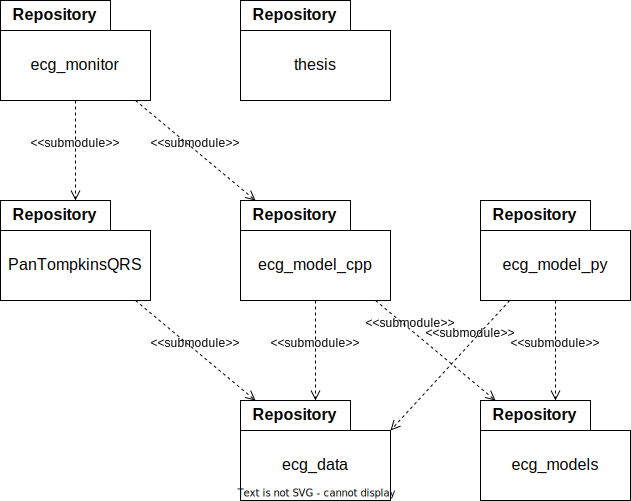
\includegraphics[width=\textwidth]{../assets/repositories.drawio}
    \bicaption{项目包含的Git仓库}{Git repositories of the project}
    \label{fig:repositories}
\end{figure}

\subsubsection{thesis}\label{subsubsec:repo-thesis}

这是本篇论文所在的仓库。论文本身作为项目文档,也被视为本项目的一部分。该仓库包含论文的\LaTeX 源码,以及论文中引用的图片等资源文件,还有自动格式化、依赖版本管理、自动构建测试、自动发布新版本等持续集成配置。

论文与应用本身的代码是分离的,所以论文的仓库与应用的仓库之间没有任何子模块关系。此外,论文仓库以Git子树的形式包含了论文模板\footnote{\url{https://github.com/Koyamin/ECNUThesis-Undergraduate}},没有使用Git子模块是因为基于模板进行编写后只需要直接提交至主仓库,不需要向子仓库推送,这与~\ref{subsec:git-submodule} 节所述的情况不同。

\subsubsection{ecg\_monitor}\label{subsubsec:repo-monitor}

这是应用的主体仓库。该仓库包含基于Flutter框架编写的Dart代码,以及相关的各种配置文件等。仓库的命名与应用的包名一致,因此按照Dart对包名的相关限制使用了小写下划线的命名风格,而非Git仓库常用的小写连字符。为了保持项目各个仓库之间的一致性,其他仓库(除PanTompkinsQRS外)也都使用了小写下划线的命名风格。

为了方便调用C++代码,该仓库以Git子模块的形式包含了PanTompkinsQRS和ecg\_model\_cpp两个子仓库,这两个子仓库分别提供了Pan-Tompkins算法和基于LibTorch的心电图智能分析算法的实现。

\subsubsection{PanTompkinsQRS}\label{subsubsec:repo-qrs}

这是应用中用于实现Pan-Tompkins算法的仓库。该仓库是rafaelmmoreira编写的Pan-Tompkins算法的C语言实现\footnote{\url{https://github.com/rafaelmmoreira/PanTompkinsQRS}}的复刻(fork),在原始版本的基础上根据项目需要进行了一些修改。出于对原作者的尊重,该仓库的名称与原作者的命名保持一致,因此与项目内其他仓库的命名风格不同。

该仓库被ecg\_monitor所包含,并且为了方便测试而将ecg\_data包含为了子仓库,后者提供了一些测试用的心电图数据,用作测试时的输入。

\subsubsection{ecg\_model\_cpp}\label{subsubsec:repo-cpp}

这是应用中用于实现基于LibTorch的心电图智能分析算法的仓库。该仓库是ecg\_model\_py仓库的C++实现,使用了LibTorch作为框架。

该仓库被ecg\_monitor所包含,且包含了ecg\_data作为测试输入数据,还包含了ecg\_models作为与ecg\_model\_py共享的模型文件以及测试预期输出。

\subsubsection{ecg\_model\_py}\label{subsubsec:repo-py}

这是基于PyTorch实现的心电图智能分析算法的所在仓库。该仓库以算法的原始版本作为初始提交,在此基础上根据项目需要进行了修改。

Python版本的算法并不直接被应用调用,因此该仓库不是其他仓库的子模块。该仓库包含了ecg\_data作为测试输入数据,将与ecg\_model\_cpp共享的模型文件保存在ecg\_models,并将PyTorch版本的算法输出也写入ecg\_models子模块以便与ecg\_model\_cpp共享。

\subsubsection{ecg\_data}\label{subsubsec:repo-data}

该仓库存储了各算法仓库用作测试输入的心电图数据,以及从公开数据库下载心电数据并转换格式的相关代码。该仓库中的数据由仓库内的代码写入,被上述三个算法仓库所读取。

\subsubsection{ecg\_models}\label{subsubsec:repo-models}

该仓库存储了TorchScript模型文件,以及模型在测试输入下的输出结果。该仓库的内容由ecg\_model\_py写入,被ecg\_model\_cpp读取。因为模型文件较大(60多MB),且不被Pan-Tompkins算法所需要,所以该仓库与ecg\_data进行了分离。


\section{Pan-Tompkins算法的实现}\label{sec:pan-tompkins}

本应用为用户提供了实时的心率显示。因为所使用的基于LibTorch的算法无法实时给出心电分割结果,所以有必要另外使用一种实时在线算法来进行心率的统计。

Pan-Tompkins算法\cite{panRealTimeQRSDetection1985}可以用于检测心电图中的QRS波群。一次正常的窦性心律的组成如图~\ref{fig:sinus-rhythm} 所示,其中的QRS波群位于心电图中最明显的尖峰处。此功能使得Pan-Tompkins算法非常适合用作心率测量。

\begin{figure}[ht]
    \centering
    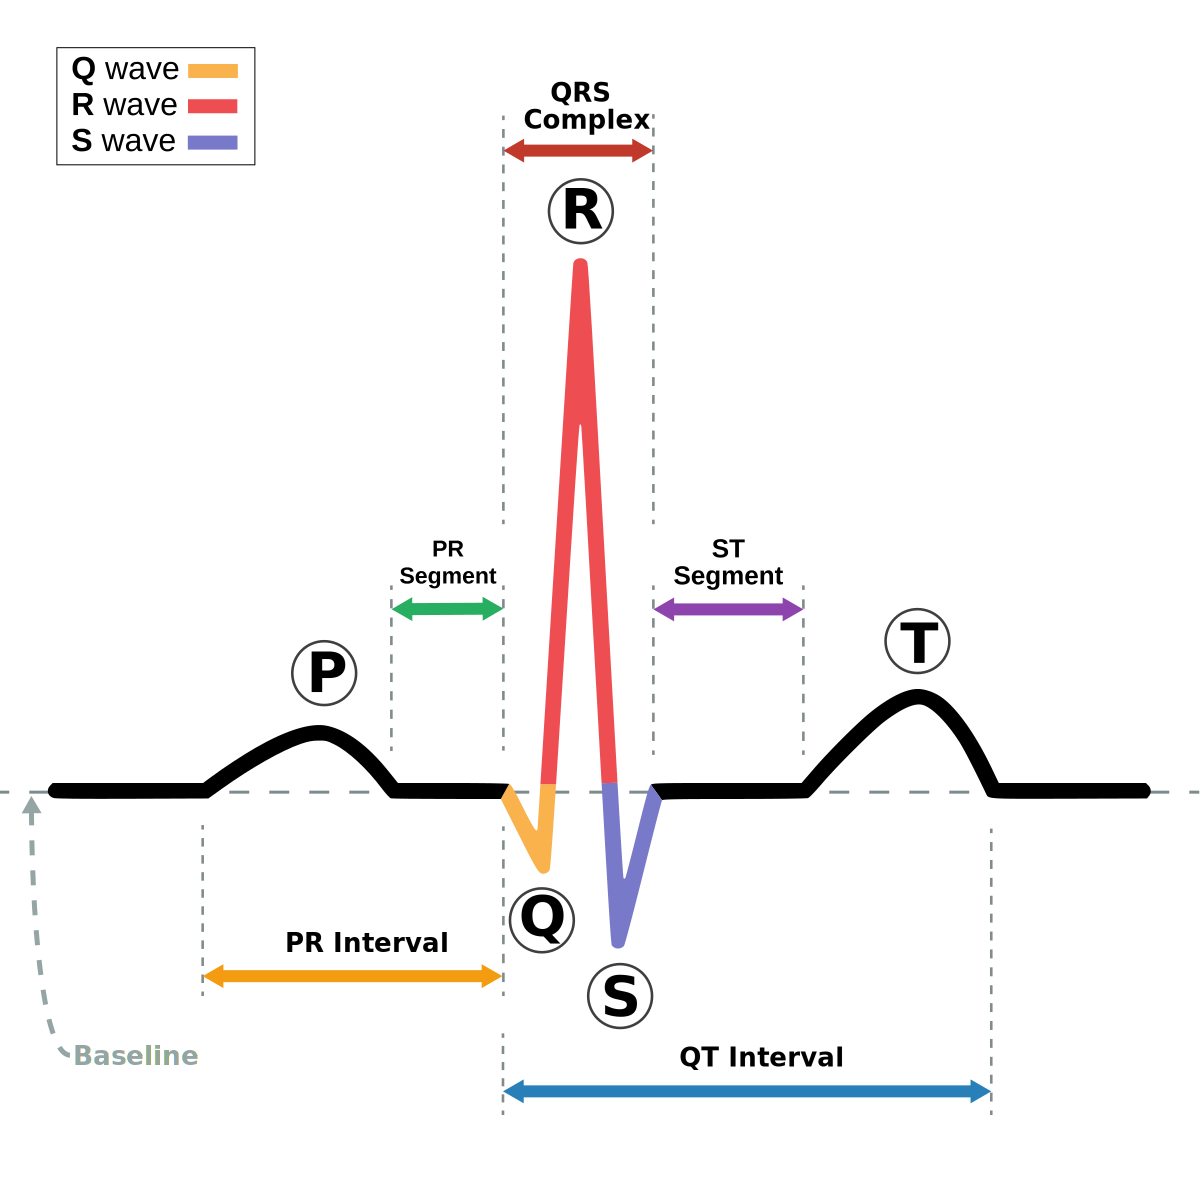
\includegraphics[width=.75\textwidth]{../assets/SinusRhythmLabels}
    \bicaption{正常窦性心律的心电图}{ECG of a heart in normal sinus rhythm}
    \label{fig:sinus-rhythm}
\end{figure}

该算法是心电分析中最经典的算法之一。于1985年被提出后,有许多人对其进行了各种各样的改进。由于算法的原始版本已经有很高的准确率(原作者给出的统计结果为99.3\%),同时本应用仅将其用作实时心率检测,没有很高的准确率要求,所以出于实现较为简单的优势而直接使用了原始版本的算法,而非其他人的改版。

由于Pan-Tompkins算法的应用非常广泛,多年以来,已经有大量开发者用各种语言各种方式对其进行了实现。为了不进行无意义的额外工作,本项目在Pan-Tompkins算法的实现过程中并非从零开始编写,而是基于已有的实现进行了修改。经过检索对比,发现rafaelmmoreira为该算法编写的C语言实现\footnote{\url{https://github.com/rafaelmmoreira/PanTompkinsQRS}}的代码质量较高,以MIT协议开源,并提供了充分的注释文档以方便理解,因此本项目以该版本实现为基础按项目需要进行了一些修改。

首先,将该实现由C语言迁移至了C++。除了将在C++中无法通过编译的特性(比如动态数组大小)进行了修改外,还将一些内容的写法改为了C++中惯用的写法,包括将使用宏定义的常量改为 |constexpr|、将 |fopen| 相关的写法替换为 |std::ifstream| 等。

之后,对该实现的输入输出方式进行了修改。在原始版本的算法中,程序开始运行时会打开两个文件作为输入输出。为了方便Dart调用,需要将输入输出方式改为直接通过参数和返回值进行。原作者已经考虑到需要修改输入输出方式的需求,并从算法中提取出了 |dataType input()| 和 |void output(int out)| 两个函数。原始情况下,算法会在需要读入新数据时调用 |input|,在分析结果就绪后调用 |output|,两者之间并不同步,而是使用了异步回调。跨语言实现异步回调虽然并非完全不可行,但相比简单的调用后直接返回的流程更为繁琐,且没有太大收益。经过分析,发现该算法实现的主体部分是一个无限循环,在循环的开头会调用 |input| 获取采样点数据,在循环中间的多处会调用 |output| 后进入到下一次循环。为了将其改为单次调用后直接返回的方式,将该循环的内容提取为了另一个函数,并将需要在循环之间保留的状态由函数内的局部变量暂时改为了全局变量。同时,将输入与输出进行同步,以略微降低算法精度为代价获得了更及时的检测结果。

在该实现的原始版本中,采样率是以常量的形式硬编码在算法之中的。但是,实际调用该算法进行分析时,可能会以不同采样率的数据进行输入。一种可能的方式是将算法复制多份修改常量后分别编译,但比较繁琐。另一种方式是将该常量改为算法的参数,从外部传入。由于算法中有很多常量和变量的值与采样率有关,因此为了方便将其作为参数,将上一个步骤中提取出的全局变量与函数封装成为了类,并将采样率作为该类的构造函数的参数。这一改动也解释了之前为什么选择将C语言的实现迁移至C++而非直接使用C语言进行重构,这样可以利用C++的强大特性来简化代码的编写难度。

在最终版本的算法中,对外提供了两个函数作为接口,分别是 |void init(int fs)| 和 |bool panTompkins(float sample)|。包含相关状态与方法的类被简单地命名为 |PanTompkins|。程序中维护了一个 |std::optional<PanTompkins>| 类型的全局变量,用于存储算法的状态。在调用 |init| 时,如果全局变量目前为空或者存储的算法的采样率与传入的参数不同,则会创建一个新的算法实例并存储在全局变量中;如果全局变量目前不为空且存储的算法的采样率与传入的参数相同,则不会创建新的算法实例,而是直接复用旧的实例,以减少不必要的开销。由于用户通常不会频繁更换使用不同采样率的设备,此优化的效果是比较明显的。在调用 |panTompkins| 时,会断言当前全局变量不为空,也就是要求调用者必须先调用过 |init| 再调用此方法;之后,会将传入的采样点数据转发至算法实例的对应方法,该方法会返回一个布尔值,表示是否检测到了新的QRS波群。

在算法的测试过程中,发现其偶尔会对于同一个心拍输出两次或更多相近甚至相邻的 |true|,导致计算出的心率可能会突然提升至每分钟上千次。由于难以确定是在算法的哪一处出现了问题,所以在算法之外对于其输出结果设计了两层额外修正,而没有修改算法内部的执行逻辑。第一层修正是为算法输出的QRS波群设置最小间隔,该间隔的计算方式如下:

\[
    leastSamplesBetweenQrs = \frac{60}{maxHeartRate} \times fs
\]

其中,\(leastSamplesBetweenQrs\) 表示连续两个QRS波群之间至少需要间隔的采样点数。当算法返回了 |true| 时,会将当前的采样点与上一次检测到QRS波群的采样点进行比较,如果两者之间的采样点数目小于 \(leastSamplesBetweenQrs\),则会忽略该检测结果,否则会将当前的采样点作为最后一次检测到QRS波群的采样点。60表示一分钟的秒数,\(maxHeartRate\) 表示最大心率(单位bpm),\(fs\) 表示采样率(单位Hz)。关于人类的心率上限,最流行的说法是220减去年龄。考虑到患者应该不会在心率超出此上限的情况下还有使用本应用观察自己心率的需求,同时为了不需要获取患者的实际年龄就可以运行算法,在实现中将\(maxHeartRate\) 设置为了常量220。经过测试,该修正可以有效地解决算法输出的QRS波群之间间隔过小导致心率上千的问题。

此外,在最终的心率显示部分也增加了一层修正。该层修正是在前述过滤方式未能完全排除算法的错误输出的情况下的缓冲。考虑到人类的心率的变化应该是相对平滑的,不太可能在相邻几个心拍之间产生非常大的变动,应用在最终将心率计算结果展示给用户的时候会先与之前的结果进行比较,如果相差超过10bpm,则会将显示结果改为上一次结果加上或减去10bpm(取决于心率是突然上升还是突然下降),但不改变底层数据的实际值。通过这种方式,可以有效地避免因为算法的错误输出导致心率突然上升或下降的情况,同时在心率真的在短时间内发生了较大的变化时,也能够在数次心拍后将所显示的心率恢复到正确的值。

应用对于心率的计算是根据最后两次检测到的心拍的间隔时间,所以另一个考虑过的修正方案是使用较多心拍之间间隔的平均值来计算心率。这种方案的效果与原理和上一段说明的方式类似,都是对心率变化进行平滑处理,滤去突变。相比起来,这种方案需要将过去的更多心拍纳入计算,但相比之前的方法在效果上没有明显的优势,所以在实现中没有采用。


\section{智能检测算法的移植与优化}\label{sec:ai}

Pan-Tompkins算法只能给出心拍的位置,但无法确定心拍的类型。同时,其作为在线算法,虽然有能实时输出结果的优点,但准确率相较离线算法也更低一些。由于用户对于分析报告的查看没有实时性非常高的需求,因此应用使用基于人工智能的另一种算法来对心电数据进行分析。

所用算法的原始版本使用Python实现。对于将其迁移至C++的过程,考虑过两种方案。其一是先将Python代码原样翻译成C++,再对C++代码进行重构以满足项目需求;这种方案的优点在于比较容易按C++的风格对代码进行重构,而缺点在于需要翻译的代码量比较大故容易出错,而且其中包含很多最终不需要使用的代码以及难以在C++中找到对应替代的依赖项。因此,本项目采用了与之相对的另一种方案,即先对Python代码进行重构,再将重构后的代码原样翻译成C++;这种方案可以最小化翻译代码步骤的工作量,并可以事先编写单元测试来保证重构过程不会破坏代码的正确性;其主要缺点则在于需要在重构过程中注意避免使用难以在C++中实现的特性,比如对同一变量进行多次不同类型的赋值\footnote{严格来说,这可以通过std::variant或union等方式实现,但会失去一部分静态类型检查的好处。}等。

首先执行的步骤是对代码的格式进行统一。在原始版本的代码中,命名、空格等格式均混合使用了多种风格,不便阅读。因此,首先对代码使用Black工具进行了格式化,使得代码的空格、换行等风格更加统一。然后利用PyCharm的重构功能对代码中变量、函数等的命名进行了修改,使其遵守Python官方的PEP-8规范中对命名的相关要求。此外,在该步骤中也移除了PyCharm能够直接检测出的一些未被使用的导入项;自动优化导入后发现代码无法继续正常运行,排查发现代码中使用类似反射的方式使用了部分导入的内容,因此未被PyCharm检测到;为该类实际上被使用的导入项添加了注释,以抑制PyCharm的误报。

之后进行的是对算法的输入输出方式的优化。在原始版本中,算法的每个步骤都是从磁盘文件读取数据作为输入,之后把其结果写入另一个磁盘文件。这种方式虽然编写简单,但会导致数据在各个步骤之间的流向非常不清晰,并且在性能上有所损耗。最关键的是,这种输入输出方式使得难以为各个步骤编写单元测试。因此,优先调整了代码中数据的传递方式,使之仅在主函数中从磁盘文件读入,之后各个步骤均通过参数与返回值直接传递,最后再在主函数中将最终结果写入磁盘文件。这样以来,就可以通过替代主函数来为算法编写单元测试,方便后续重构。该步骤完成之后,对比了最终的磁盘文件与原始版本的输出,发现了一些不一致,经研究讨论后发现是出于原始版本的一些bug,修复后可以得到一致的输出。据此可以判定该步骤并未破坏算法的正确性,反而修正了原本存在的缺陷,而此后的步骤都可以通过持续集成中自动运行的单元测试而非手动对比来保证算法在相同输入下的输出并未改变。

原始项目中包含非常多的代码文件,但是经过覆盖率检测,发现在算法执行的过程中大部分代码都没有被执行到。经过仔细测试、分析,发现有许多代码是多余的。于是删去了无意义的代码,这包括原项目中的数个目录、一些文件、以及某些文件中的部分代码行。之后,发现有部分模型等资源文件也未被读取过,将这些文件也进行了清理。完成对于未使用文件的清理后,对项目中各个文件的位置进行了调整,将代码文件与资源文件等分别移至单独的目录中,方便后续继续重构。

该算法原本使用了一段长达24小时的动态心电数据进行测试,这可以较为充分地测试算法对于各种类型的心电数据的表现,但也导致测试时间很长,单次执行需要数分钟,在性能较差的持续集成环境下甚至需要更久。由于代码每次进行更改时都要重新运行测试以保证正确性,为了减少在测试步骤的等待时间,提高开发效率,将数据截取了前10分钟来进行更快速的测试。

下一个步骤是进行更细粒度的重构。由于原项目代码的组织结构较为混乱,为了方便后续处理,首先将所有代码文件合并至单个文件之中,去除了多个代码文件之间的导入。在合并的过程中以及合并完成后,发现各个文件中存在部分逻辑相似甚至完全相同的代码,对这些重复的代码进行了合并,提取了共用的方法。并且,对一些未使用的参数进行了删除;对在所有调用中均传递了相同值的参数(比如重采样的目标采样率被固定为250Hz)进行了简化,仅作为全局常量,而不在层层调用中进行传递。在该步骤中,也对方法中一些不符合正常编码习惯的写法进行了替换,比如将 |flag == False| 改为 |not flag|(C++中为 |!flag|)、手动打印错误消息改为抛出异常等。此外,对一些与最终结果无关的调试代码,比如基于 |tqdm| 打印算法执行进度的代码,进行了删除,并消去了相关依赖项。最后,将简化完毕的代码重新按执行步骤分割为多个模块,分别存储于单独的代码文件供主函数调用,并将仅在某一步骤使用的函数设为模块级别的私有函数,以提高代码的内聚性。

将代码迁移至C++前的最后一个重构步骤是为参数、变量、返回值等添加类型标注。虽然Python是动态类型语言,但通过类型标注,仍然可以获得静态类型检查的优势。在该步骤中,使用Mypy工具进行了严格的检查,固定了每个变量、参数的类型,对同变量多次赋值为不同类型的情况进行了变量拆分。在这一步骤中也借助类型检查发现了原始代码中的一处笔误,该笔误所处代码所代表的情况刚好在测试数据的执行过程中未出现过,所以之前未被发现。之后,对错误进行了修正。

得益于上述的重构,以及LibTorch、NumCpp等库的接口设计的友好性,迁移过程的工作基本都在于翻译语言功能,很少涉及代码逻辑的修改。然而,在将代码原样翻译成C++后,发现在原本在Python中可以正常使用 |torch.load| 加载的模型文件无法在C++中使用 |torch::load| 读取。检索并查阅相关资料后,发现需要先将模型转换为TorchScript格式以消除Python依赖。在转换过程中,为了适应TorchScript的限制,对模型代码进行了微小重构,如将 |for| 循环进行展开等。

在迁移过程中编写的LibTorch相关代码是在Linux环境下进行调试的,这是考虑到在移动端调试C++代码较为不便,并且C++代码具有跨平台性,在Linux下能够正常运行应该就意味着可以在其他平台也正常运行。不过,在将于Linux平台下调试完成的代码移植至移动平台时还是遇到了麻烦,其原因在于C++的跨平台性仅在源代码级别成立,而编译后的二进制文件并不能跨平台使用。而在该部分算法的各种依赖项中,LibTorch的分发方式与其他依赖不同,虽然官方也提供了开源代码,但主要的安装方式是下载并解压预先编译好的静态链接库以及相关的头文件等。但是在官网的下载页面\footnote{\url{https://pytorch.org/get-started/locally/}}中,只提供了三个桌面端系统的LibTorch下载,而没有提供移动端的LibTorch。

为了获得能在移动端使用的LibTorch,考虑过两个方案,一是从源代码自行编译,二是寻找已经编译好的版本。由于LibTorch项目规模庞大,自行编译的方式繁琐且耗时,所以优先考虑了使用已经被编译好的版本。在经过了一些寻找与尝试后,发现PyTorch官方提供的PyTorch Mobile中存在LibTorch的相关文件;事后想来这是很自然的,因为PyTorch的各种版本都是为其底层的C++实现提供其他语言的接口,那么LibTorch作为C++版本的接口也很可能会在其中使用到。在移动端的构建过程中,首先将PyTorch Mobile作为依赖项正常下载,然后并不直接使用,而是将其解压并将其中的LibTorch头文件和链接库复制至构建目录中,在C++的编译过程中对相关的头文件目录进行包含并将其链接库与算法代码进行链接。


\section{心电模块的实现}\label{sec:ecg}

\subsection{实时心电界面的实现}\label{subsec:real-time-ui}

实时心电界面的整体外观如图~\ref{fig:real-time} 所示。

\begin{figure}[ht]
    \subcaptionbox{心率检测中}{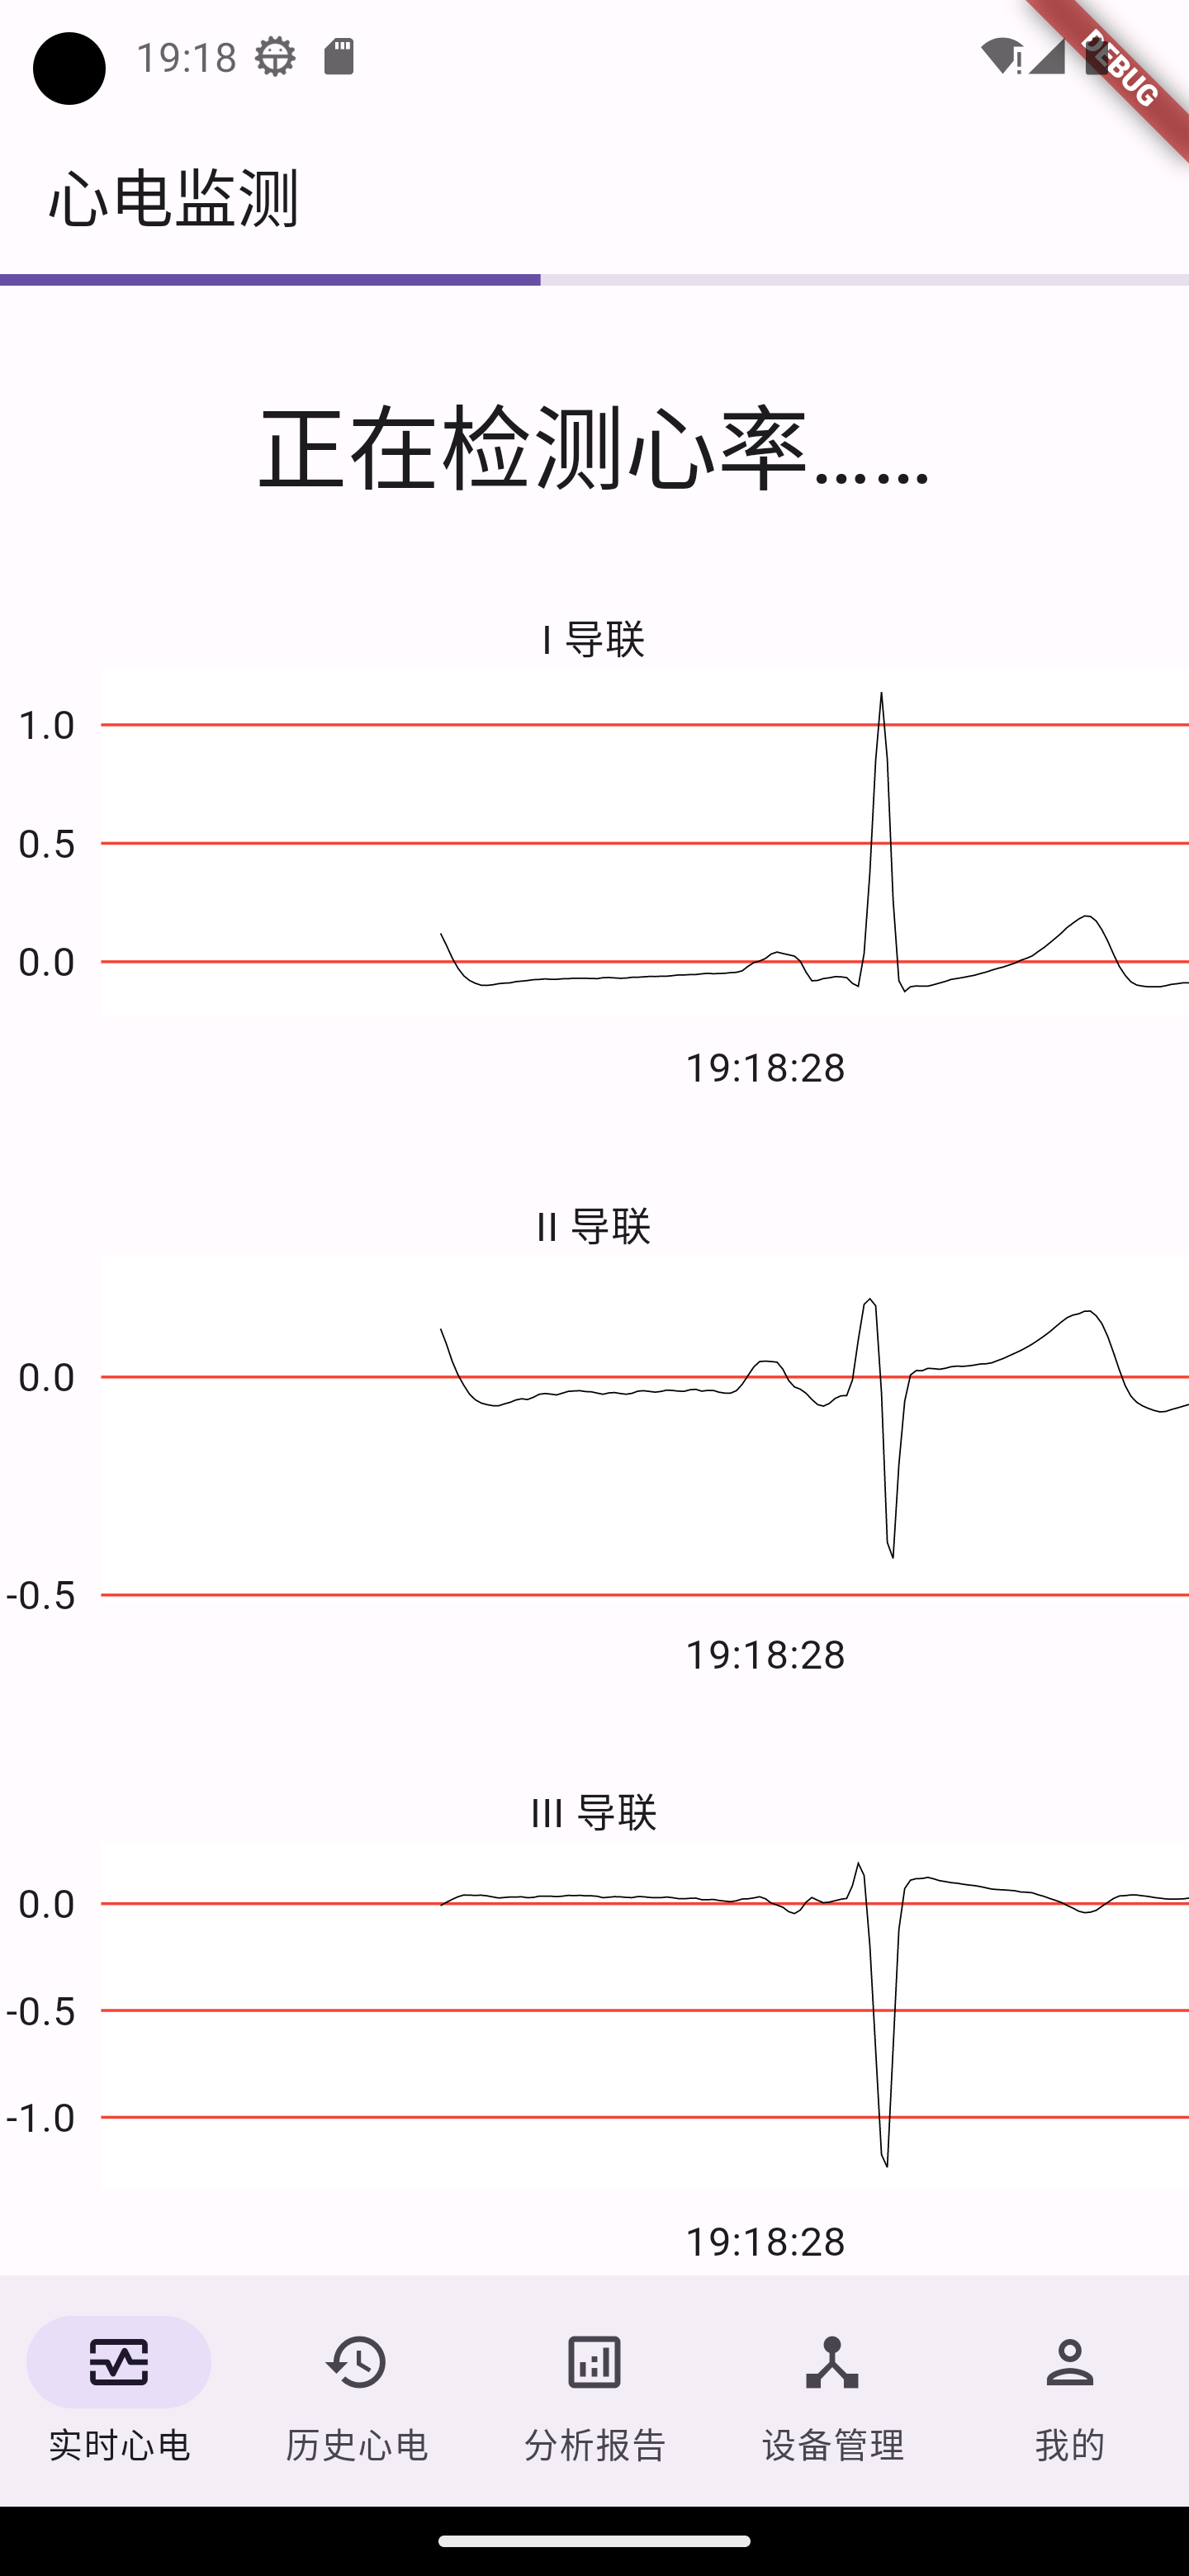
\includegraphics[width=.33\textwidth]{../assets/real-time-learning}}
    \subcaptionbox{正常状态}{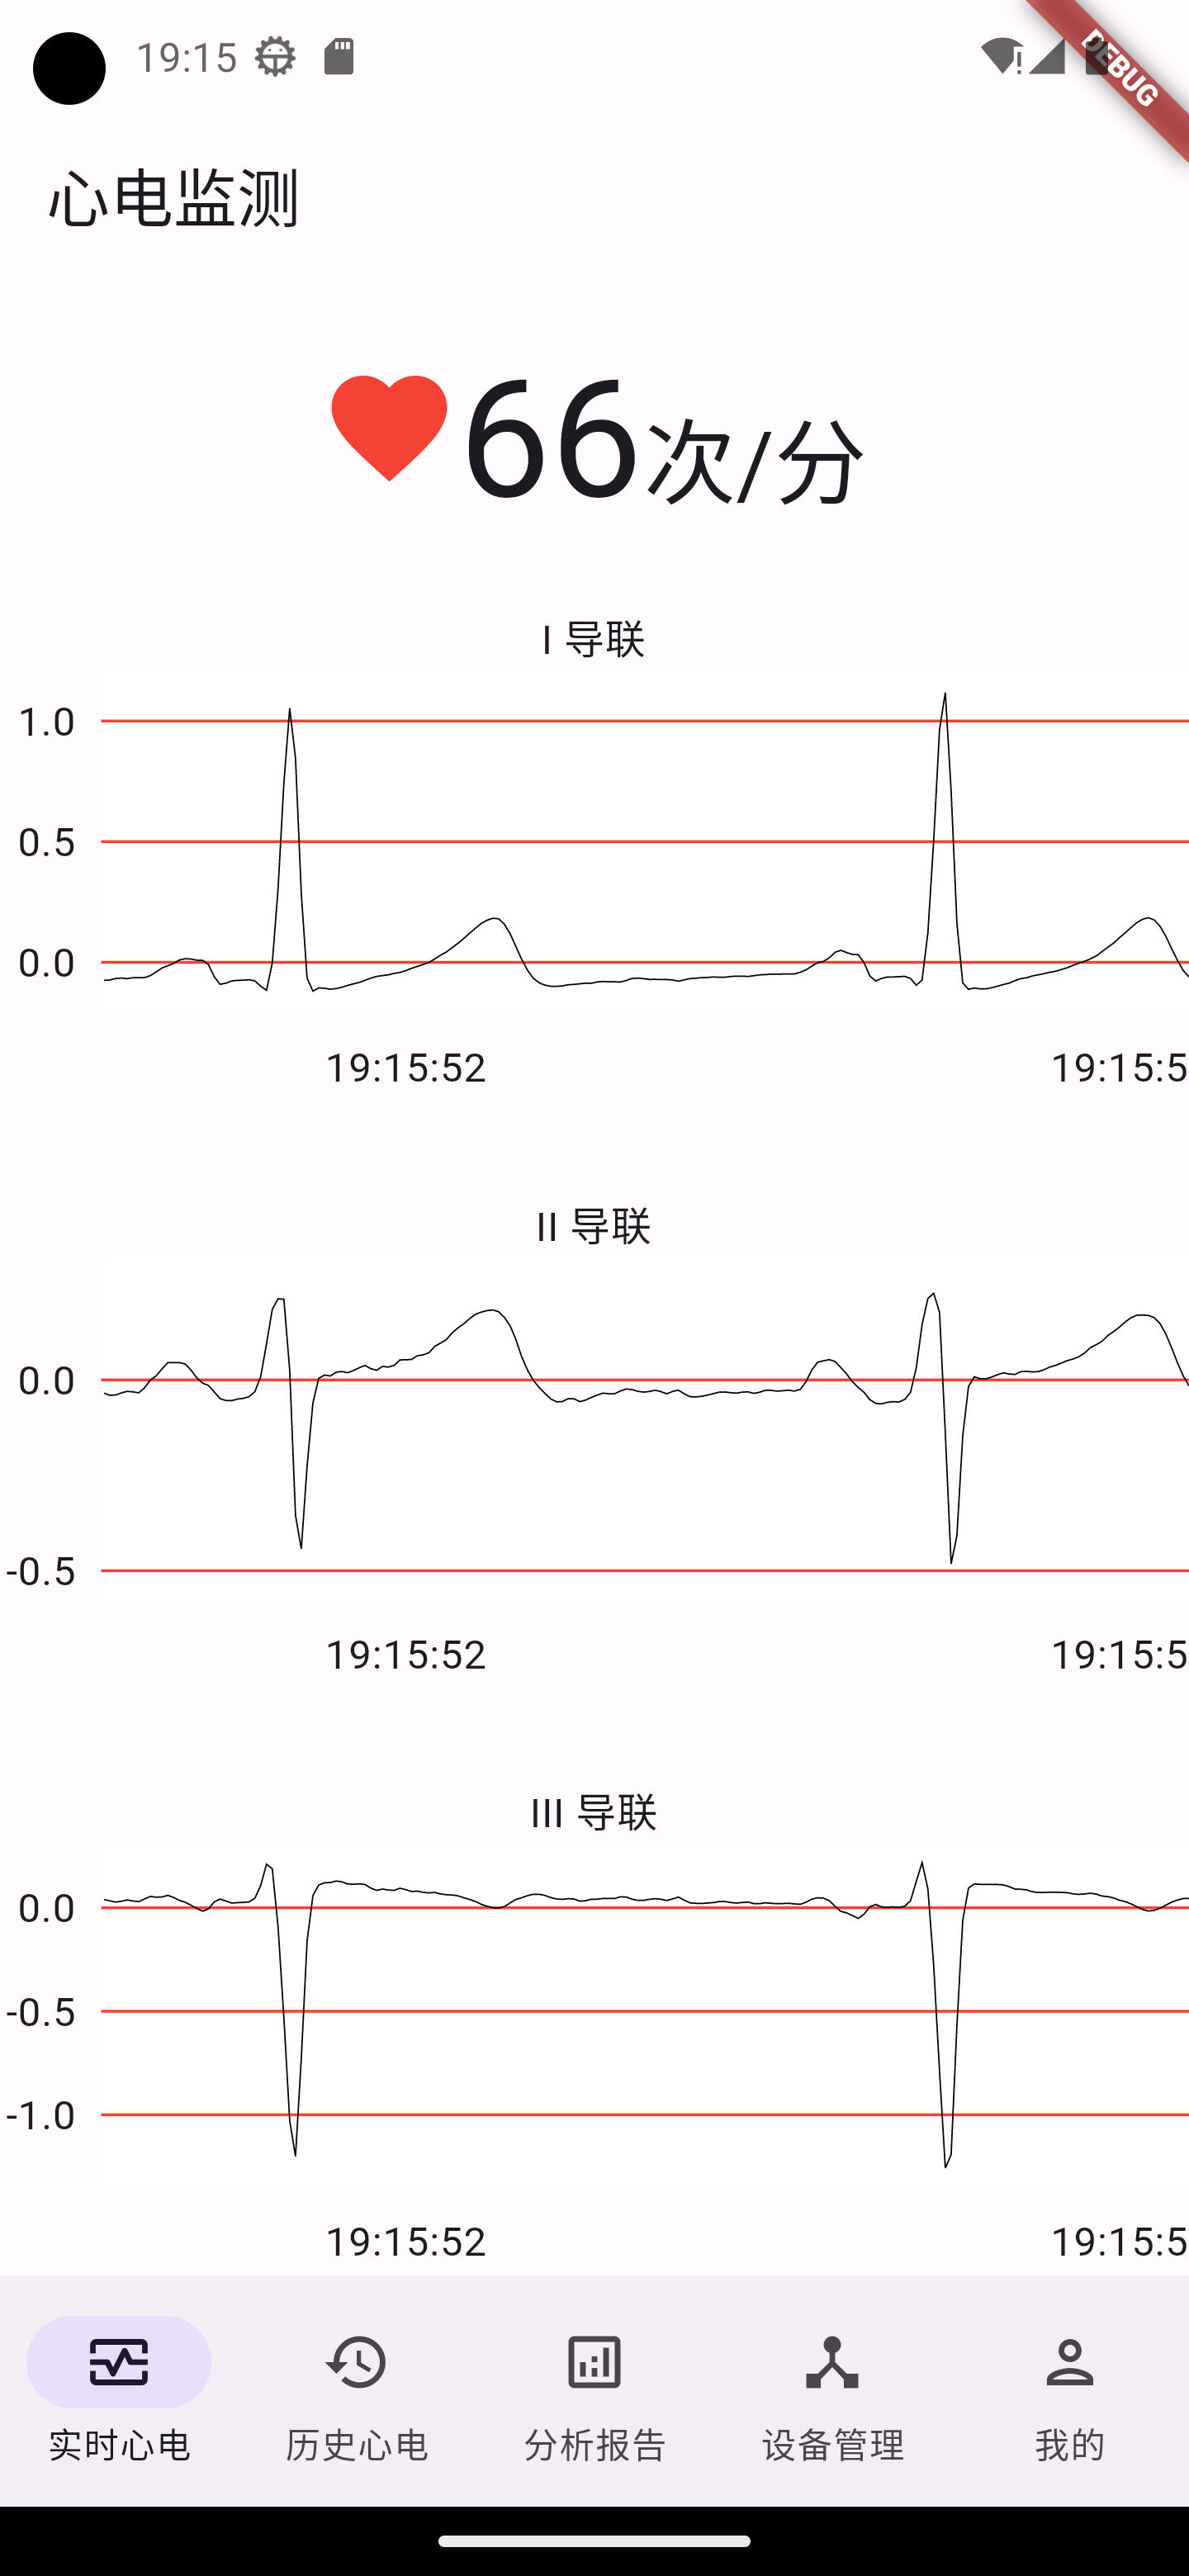
\includegraphics[width=.33\textwidth]{../assets/real-time}}
    \subcaptionbox{设备未连接}{
\includegraphics[width=.33\textwidth]{../assets/real-time-na}}
    \bicaption{实时心电界面的截图}{Screenshot of the real-time ECG page}
    \label{fig:real-time}
\end{figure}

实时心电界面的主体可以分为心率和心电图两大部分。另外,在整个应用的最上方显示了应用的名称,最下方显示了应用的导航栏,导航栏提供了应用中最主要的几个界面的入口。

\subsubsection{心率部分的界面实现}\label{subsubsec:heart-rate-ui}

实时心电界面的上方显示了用户当前的心率。

当用户刚刚佩戴上或连接上心电监测设备的时候,由于缺少数据,心率无法立即获得。在这种状态下,心率部分会显示“正在检测心率……”作为占位符,并且上方会显示一个线状的进度条。Material规范中规定了两种类型的线状进度条,分别表示确定的和不确定的进度。因为心率检测所需的时间可以大致确定,所以此处使用了确定进度的版本,进度条的已填充长度占比表示心率检测的预测进度。进度条的使用可以向用户提供检测进度的视觉反馈,虽然并不能在实际上加快检测速度,但由于减少了不确定性,仍然可以减少用户在等待过程中的焦虑感与沮丧感,起到了与加快检测速度类似的作用。反之,如果在系统正在工作的过程中不为用户提供指示,比如某些网站在上传作业文件时的实现,即使是在只需要等待数秒的情况下,用户也会感到焦虑与沮丧,在更长时间后甚至会由于缺乏对任务最终可以完成的信心而感到挫折并放弃使用。进度条虽然只是个简单的组件,但对于软件的易用性和用户体验来说却是个非常重要的细节。

心率检测的结果可用之后,该区域则会显示心率数据。显示内容由横向排布的三个组件组成:图标、数值和单位。图标使用了一个红色的心形标志,主要起到两个作用:一是指示该区域显示的内容是心率,由于应用的性质与该界面其他元素的暗示,用户很容易理解到所示数值表示心率,所以不需要使用文本等方式进行明确说明,只使用简单的图标已经足够;二是加强该区域的视觉强调效果,由于心率区域在整个屏幕上的面积占比较少,但重要性并不显著弱于下方的心电图等元素,所以使用了这个颜色较为鲜艳的图标来将用户的注意力吸引至该区域。数值和单位使用了不同大小的字体,数值较大而单位较小。这是因为心率数值是该区域的主要内容,且不断变动,需要较为强调。而心率的单位是固定的,不会变动,而且每分钟的次数(bpm)作为最常用的心率单位已经为用户所习惯,不需要特别强调,所以使用较小的字体弱化了单位的视觉效果,以突出其他部分。三个组件在横向与纵向上整体居中,内部按文本基线对齐(即靠下对齐)。

此外,整个心率显示区域在实时心电界面上的高度占比是固定的,以免在检测完成前后以及数值变动时引起下方心电图位置的上下移动。

\subsubsection{心电图部分的界面实现}\label{subsubsec:ecg-ui}

心电图部分的界面外观参考了医学上常用的心电图纸的样式。心电图纸的整体外观在\nameref{ch:intro}部分的图~\ref{fig:ecg-paper-example} 中已经展示过,这里对其具体布局方式进行一些补充介绍。

心电图纸包含横纵交错的坐标线,通常为红色或浅红色,如图~\ref{fig:ecg-paper} 所示。每1mm一小格(用细线分隔),每5mm一大格(用粗线分隔)。横轴一小格表示40ms,一大格表示200ms。纵轴一小格表示0.1mV,一大格表示0.5mV。心电图的边缘有1mV(10mm高)的参考波形,并标注该条图像的导联名称。

\begin{figure}[ht]
    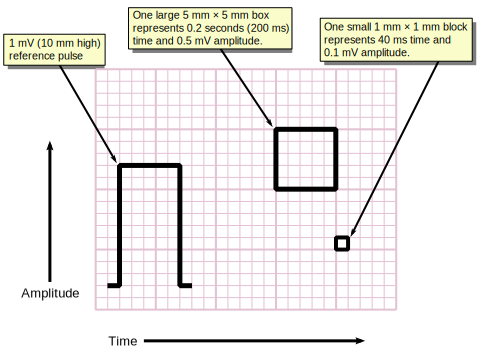
\includegraphics[width=\textwidth]{../assets/ECG_Paper_v2}
    \bicaption{心电图纸的布局}{Layout of ECG paper}
    \label{fig:ecg-paper}
\end{figure}

在应用内实时心电图的界面实现过程中,对心电图纸的元素进行了一些精简与修改。首先,由于移动设备的屏幕尺寸较小,将心电数据的显示范围进行了缩减,纵轴范围根据当前图中显示的心电数据自适应变动,以最大值加0.1mV作为上限,最小值减0.1mV作为下限。横轴范围则按照心电数据的常见电压范围进行了等比例调整,使其与纵轴比例可以保持近似对应,并在应用设置内增加了相关的选项供用户按需自行调整。之后,由于纵向坐标线在实时心电图的快速移动的过程中会产生视觉上的严重干扰,所以将其去除,改为在下方显示数据对应的时间;为了保持视觉上的协调,横轴坐标线去除了划分小格的细线,仅保留了0.5mV一条的粗线。最后,考虑到一般用户对心电图纸的参考波形的了解程度较低,加之移动设备的显示空间有限,所以将参考波形去除,改为在左侧显示电压数值,并相应地将导联名称移至心电图的正上方中央。

心电图部分在竖屏和横屏状态下有不同的显示方式。竖屏状态下,如之前所示,三个导联的心电图从上到下竖向排布在该区域。由于移动设备的屏幕宽度较窄,所以竖屏状态下可以显示的时长也较短,屏幕中每个导联通常只能显示一到两个心拍。虽然可以在应用设置中对显示时长进行调整,但在显示区域的宽度无法改变的情况下,显示更长时间的数据只能是以降低细节的可见程度为代价的。为了提供一种可以在不提高显示密度的情况下查看更长时间的数据的方式,应用在横屏状态下会改为仅显示单个导联的数据,如图~\ref{fig:real-time-landscape} 所示。

\begin{figure}[ht]
    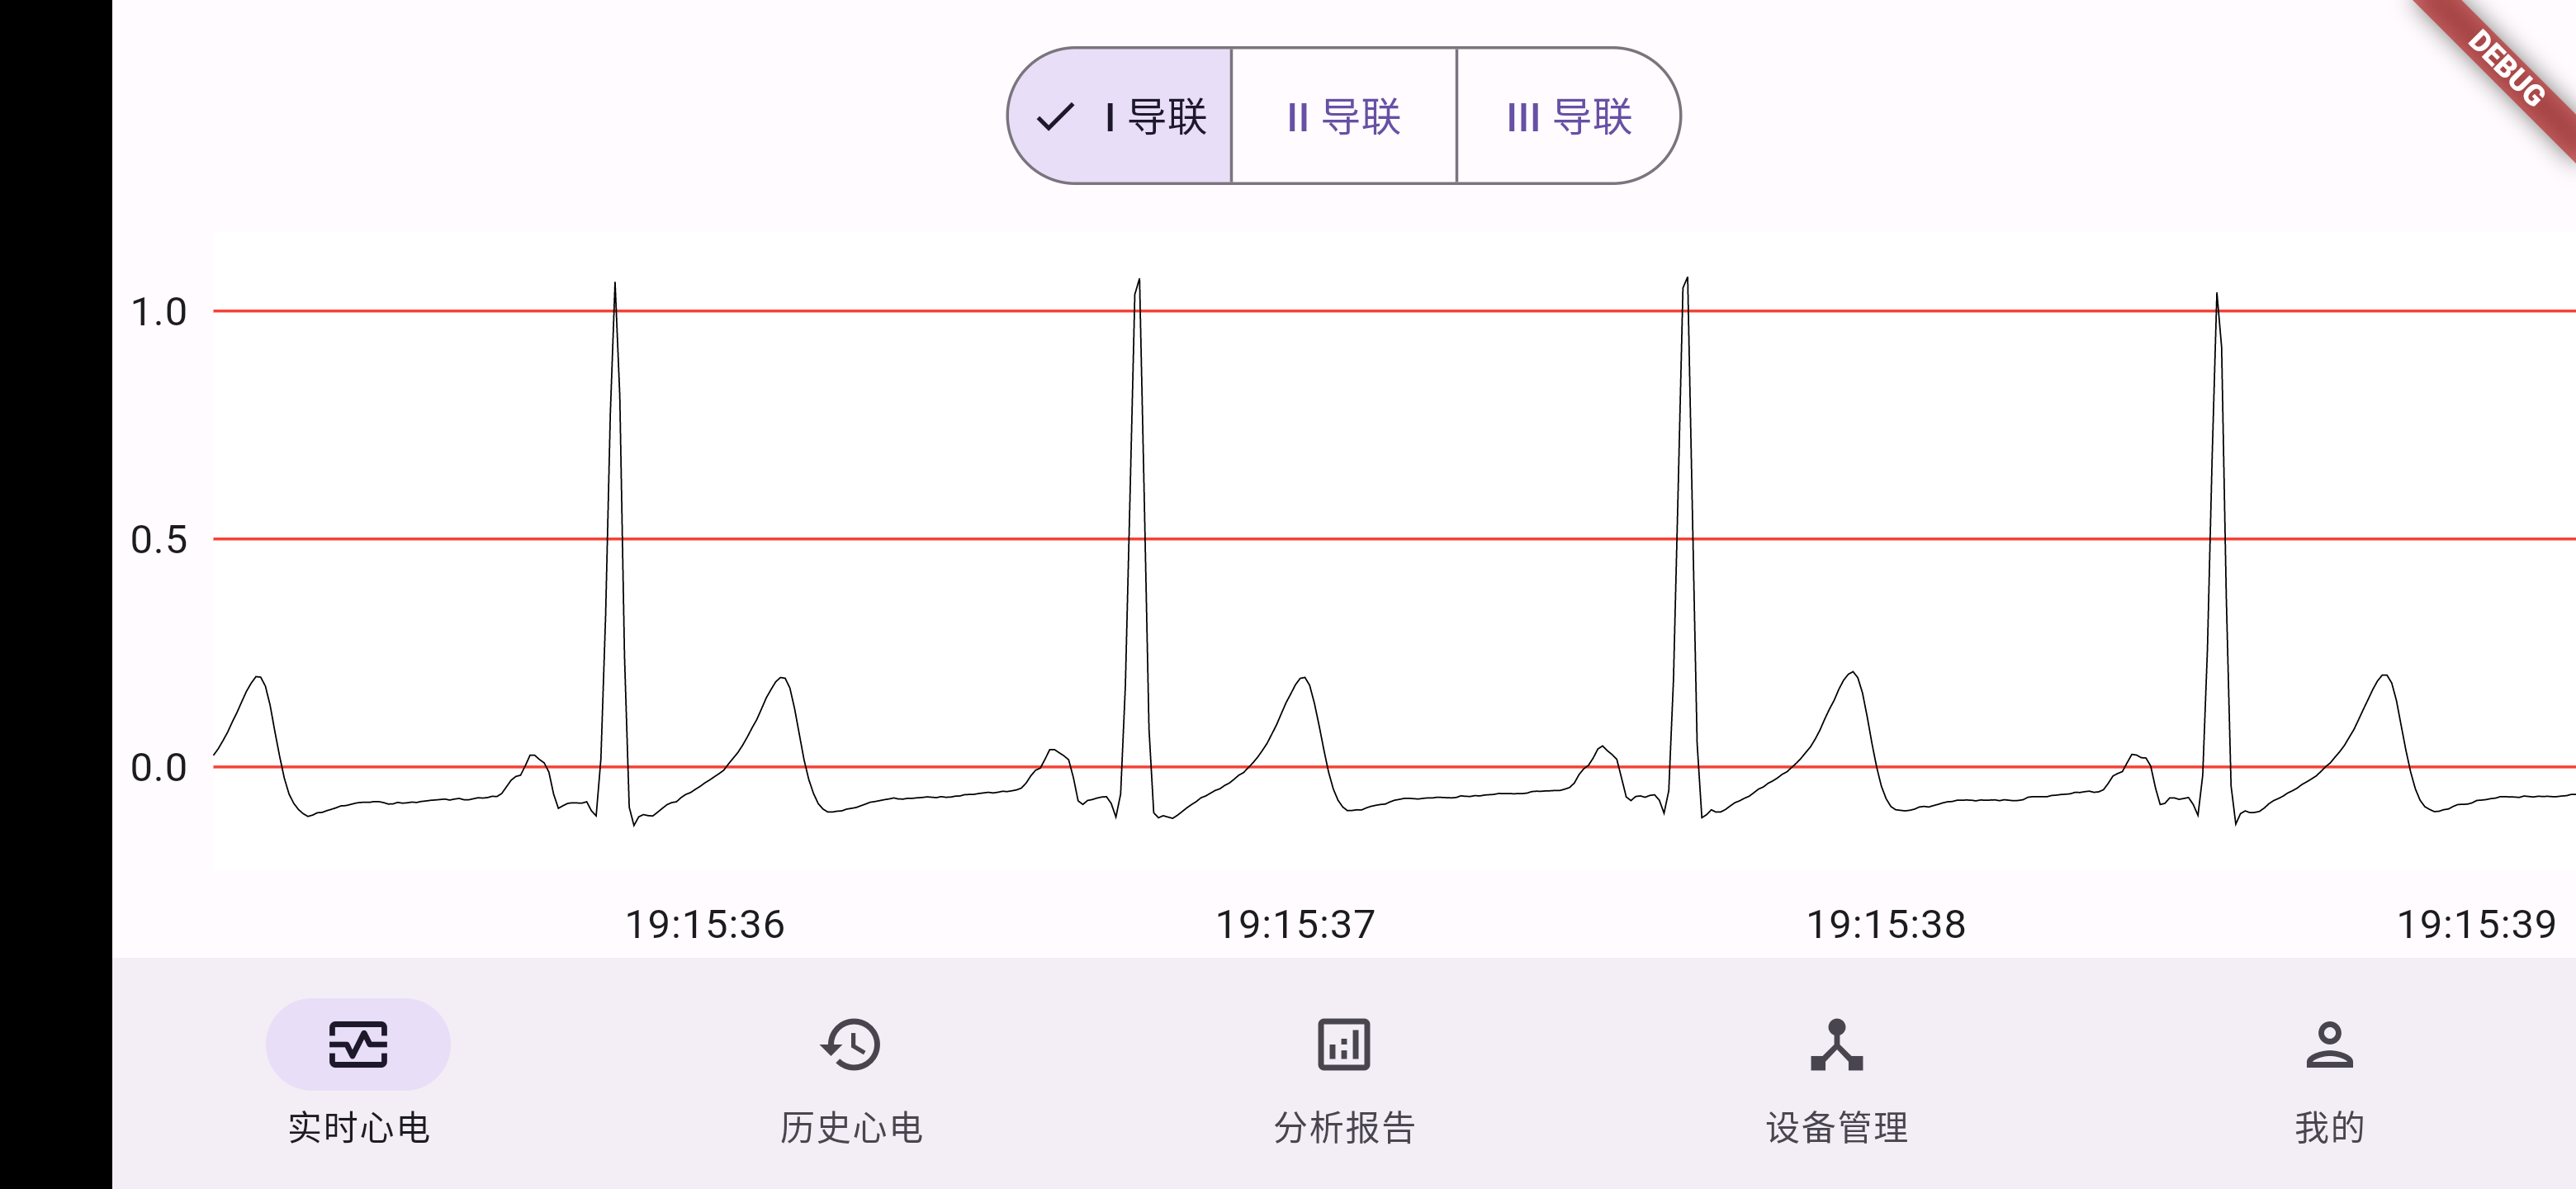
\includegraphics[width=\textwidth]{../assets/real-time-landscape}
    \bicaption{横屏状态下的心电图截图}{Screenshot of the ECG in landscape mode}
    \label{fig:real-time-landscape}
\end{figure}

在横屏状态下,应用会进入全屏状态,隐去系统自带的状态栏等元素。在应用界面内部,顶端的标题栏以及屏幕上部的心率显示区域也会隐藏,以提供更多纵向空间。心电图区域会由同时显示三个导联变为仅显示单个导联,并将心电图上方的导联名称替换为分段按钮,以便用户可以在不同的导联之间进行切换。在横屏状态下,应用在心电图之外仍然为上方的导联切换按钮与下方的导航栏保留了足够的空间。这一方面是因为Material规范要求可点击的元素必须保留足够的大小,以便用户可以轻松点击;另一方面是因为如果要让心电图在保持横纵比例不变的情况下显示更长的时间,纵向空间就需要进行相应缩减;同时,这也保证了在横屏状态下仍然可以正常使用应用的基本功能,使用户不需要在进行切换界面等操作之前先将设备恢复为竖屏状态。

\subsubsection{设备未连接状态的界面实现}\label{subsubsec:real-time-na-ui}

在设备未连接的情况下,由于无从获取实时心电数据,实时心电界面没有可供查看的实际内容。如果仅显示没有数据的空心电图,可能会使用户产生疑惑。因此,在设备未连接的情况下,应用会将实时心电界面替换为一个特殊的错误提示界面。该界面非常简洁,仅在显示区域的中央包含两个元素,竖向排布并留有一定间隔。上方以较大字体显示“设备未连接”的提示信息,下方以按钮形式提供前往设备管理界面的入口,提醒用户检查设备的状态。由于用户可能会在应用保持处于该界面的情况下调试心电设备,所以即使在心电设备尚未连接的情况下,应用也不会自动重定向至设备管理页,而是在用户手动点击按钮后才会跳转。

Material规范提供了各种外观风格的按钮。在该提示界面中,比较适用的几种风格的按钮如图~\ref{fig:buttons} 所示。

\begin{figure}[ht]
    \subcaptionbox{抬升按钮}{
\includegraphics[width=.196\textwidth]{../assets/button-elevated}}
    \subcaptionbox{填充按钮}{
\includegraphics[width=.196\textwidth]{../assets/button-filled}}
    \subcaptionbox{填充色调按钮}{
\includegraphics[width=.196\textwidth]{../assets/button-filled-tonal}}
    \subcaptionbox{轮廓按钮}{
\includegraphics[width=.196\textwidth]{../assets/button-outlined}}
    \subcaptionbox{文本按钮}{
\includegraphics[width=.196\textwidth]{../assets/button-text}}
    \bicaption{各种风格的按钮对比}{Comparison of different button styles}
    \label{fig:buttons}
\end{figure}

图中从左到右分别为抬升按钮(Elevated button)、填充按钮(Filled button)、填充色调按钮(Filled tonal button)、轮廓按钮(Outlined button)和文本按钮(Text button)。其中,抬升按钮因其阴影效果较易与其他元素之间产生不协调感,被规定为仅在绝对必要的时候,比如需要从图案背景中进行视觉分离时等特殊情况下才应使用,显然此界面并不属于应添加阴影的特殊情况。其余四种按钮的强调程度由强至弱,应当按需使用。由于该界面元素较少,所以不需要对该按钮进行较为强烈的强调,故未使用两种填充按钮。如果使用文本按钮,则视觉效果过于微弱,甚至使用户有些难以察觉到这是一个按钮。最终,选定了轮廓按钮的风格,其强调程度充足但不过度,与其他元素最为协调。

\subsubsection{应用中图标的选择}\label{subsubsec:icons}

实时心电界面在导航栏中的图标使用了常见的心电图的标志,这是根据该界面的主要内容决定的。

Material规范对于图标的设计与使用有一些相关要求。本应用为了遵循规范,使用的均是Google官方设计并开源供免费使用的图标。Google为其图标提供了各种风格的样式,常见的几种如图~\ref{fig:icons} 所示。

\begin{figure}[ht]
    \centering
    \subcaptionbox{轮廓}{
\includegraphics[width=.15\textwidth]{../assets/icon-outlined}}
    \subcaptionbox{圆润}{
\includegraphics[width=.15\textwidth]{../assets/icon-rounded}}
    \subcaptionbox{尖锐}{
\includegraphics[width=.15\textwidth]{../assets/icon-sharp}}
    \subcaptionbox{常规(旧)}{
\includegraphics[width=.15\textwidth]{../assets/icon-old-outlined}}
    \subcaptionbox{填充(旧)}{
\includegraphics[width=.15\textwidth]{../assets/icon-old-filled}}
    \bicaption{Material图标的各种风格}{Different styles of Material icons}
    \label{fig:icons}
\end{figure}

图中的前三种风格是Material 3新增的,通常应该比旧版优先使用。具体使用哪一种风格应该根据应用程序的整体界面风格来确定,比如圆润的图标使用了较多圆角,与使用较重的排版、弯曲徽标或圆形元素来表达其风格的品牌搭配得很好;尖锐的图标则带有较多直角,体现出清晰锐利的风格。本应用内的所有图标都使用了轮廓风格,这和整个应用的轻盈、干净的界面风格保持一致。

\subsection{历史心电界面的实现}\label{subsec:history-ui}

历史心电界面的整体外观如图~\ref{fig:history} 所示。

\begin{figure}[ht]
    \subcaptionbox{加载中}{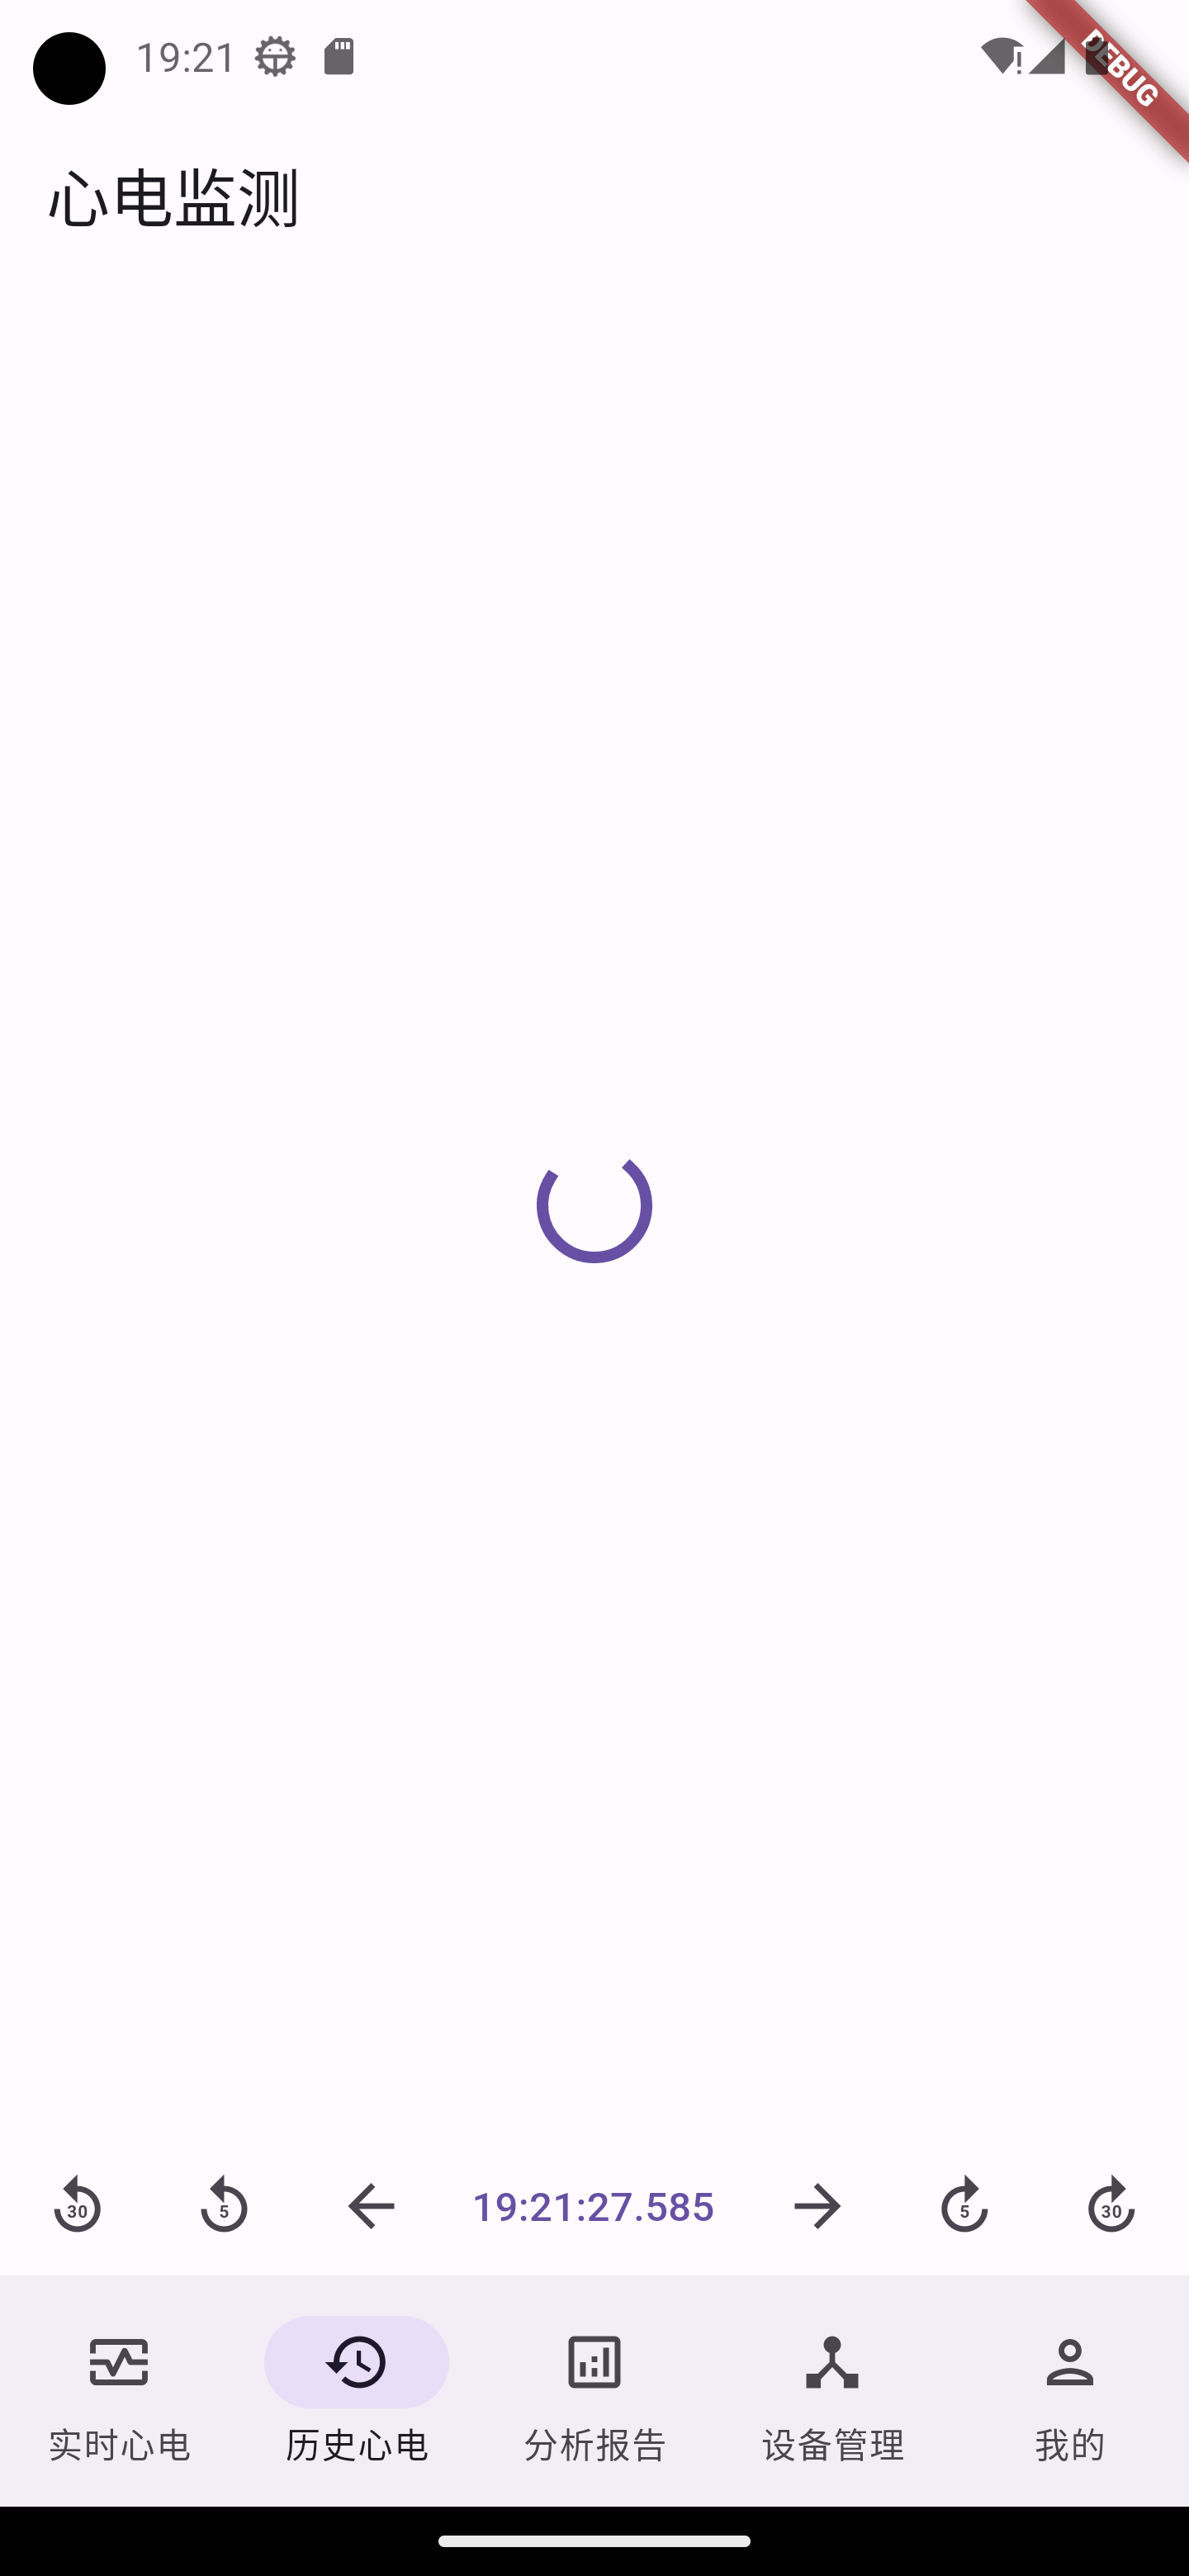
\includegraphics[width=.33\textwidth]{../assets/history-loading}}
    \subcaptionbox{正常状态}{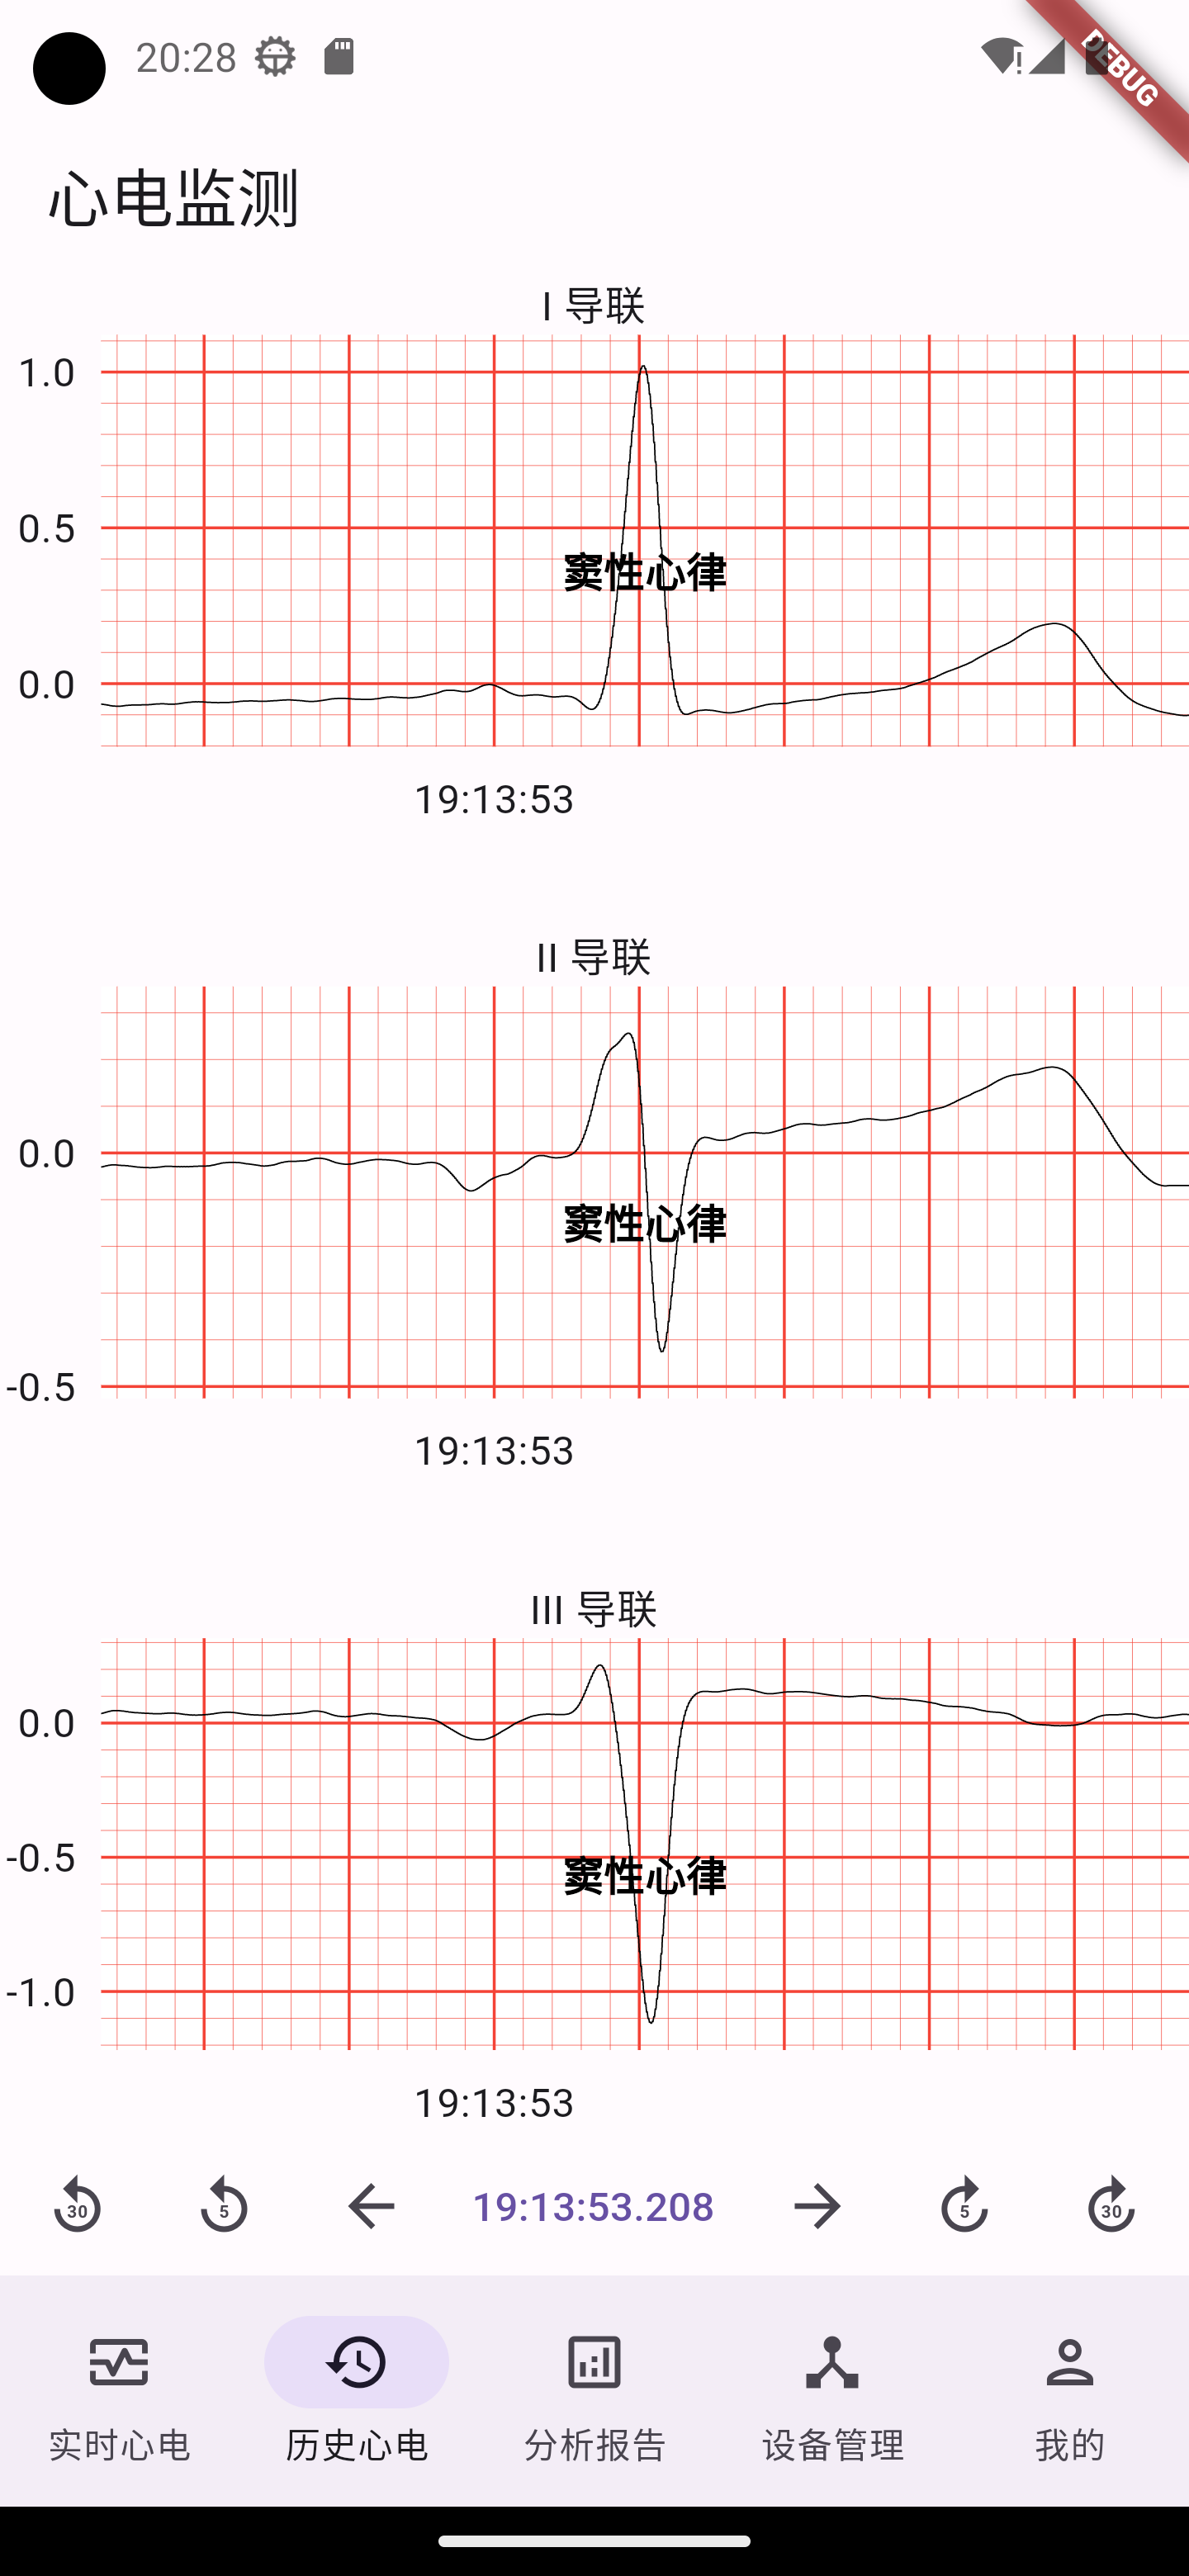
\includegraphics[width=.33\textwidth]{../assets/history}}
    \subcaptionbox{无数据}{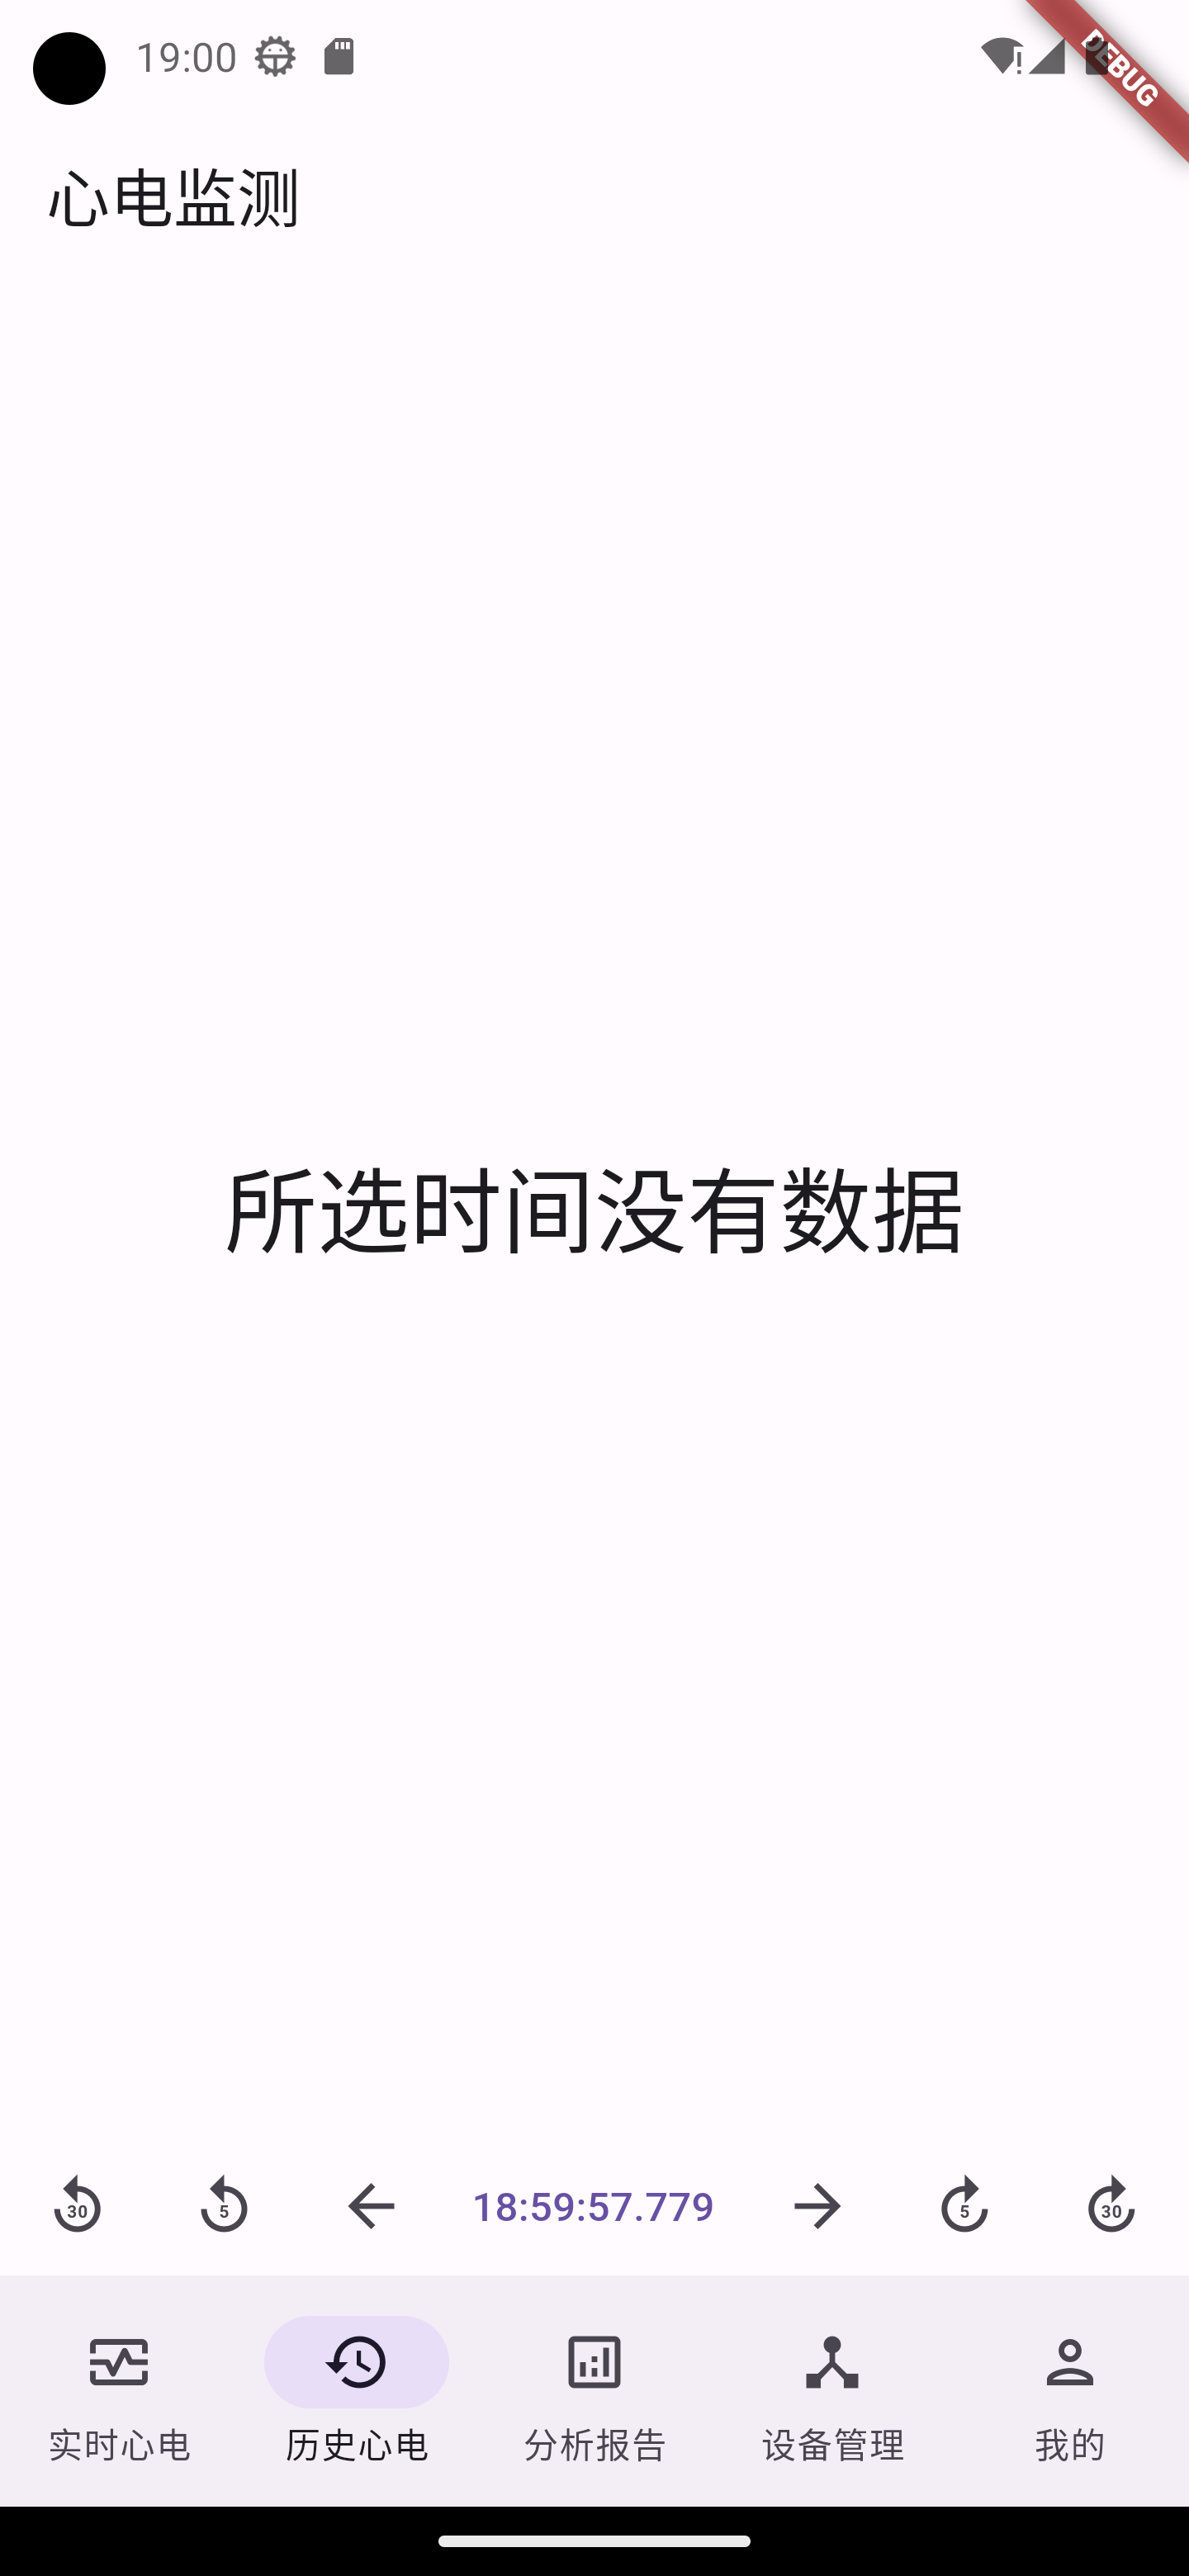
\includegraphics[width=.33\textwidth]{../assets/history-na}}
    \bicaption{历史心电界面的截图}{Screenshot of the history ECG page}
    \label{fig:history}
\end{figure}

该界面由两部分组成,分别是上方的心电图部分和下方的时间选择器部分。为了与实时心电进行区分,导航栏中的图标使用了表示历史记录的符号。

\subsubsection{心电图部分的界面实现}\label{subsubsec:history-ecg-ui}

历史心电图与实时心电图的总体界面实现方式相同,重复部分不须赘述。相比实时心电图,历史心电图因其性质而在界面外观上具有一些不同点。

首先,关于心电图背景的网格,在实时心电图中完全隐去了纵线、部分显示了横线,如上文所述是因为心电图在不停横向移动。但是在历史心电图中,图中显示的数据是静态的,在用户不调整所选时间的情况下不会发生变动。因此,没有必要在历史心电图中隐去或部分隐去背景的坐标网格。在历史心电图的界面外观中,背景的网格线与实际的心电图纸保持一致,以粗线分割大格,每大格里再以细线(实际显示为颜色较浅的线)分割为5小格。这样的界面可以使得心电图上各点的数值更加清晰,方便用户对历史心电数据进行仔细查看。

另一个显著的不同点在于历史心电图中对每个心拍的类型进行了标注。由于所使用的智能检测算法是离线算法,无法实时给出心拍类型,因此该标注在实时心电图中无法实现,仅可在历史心电图中进行查看。心拍的类型以文本形式直接显示在每个导联的心电图中对应位置的中央。一个被考虑过的替代方案是在R波(心电图中幅度最大的波)的波峰所在的点进行标注,但这需要心电图中在上方保留一些额外的空间,不太适合移动设备的较小的屏幕,而且各个导联中的波峰也并非完全同步。另一个可能的替代方案是使用颜色而非文本对心拍类型进行标注,但这种方案要么需要在屏幕上的某处显示各种颜色对应的标签而不适合小屏幕设备,要么需要用户在某个说明界面中查看并记忆各种标签的颜色而严重影响了应用的易用性,因此也没有采用。

此外,该部分区域存在两种特殊状态,分别是加载中和无数据的状态。经过对数据库的优化之后,加载中状态持续的时间很短,仅在设备性能较差、数据库索引未完成、缓存也未命中等情况同时发生的状态下才会有较长时间的加载;因此,加载中界面仅简单使用了一个圆形的不确定进度的加载动画来指示应用并未失去响应。无数据的状态则是在用户选择的时间前后内没有心电数据的情况下出现的,可能是由于用户在该时间并未佩戴监测设备,或是应用后台进程因各种原因被终止而缺失该时间的数据,也可能是用户刚刚开始使用该应用但试图查询几小时前的数据。在没有可用数据的情况下,该区域并不会显示只有背景的空心电图,而是会直接显示所选时间没有数据的提示。

\subsubsection{时间选择器部分的界面实现}\label{subsubsec:history-time-picker-ui}

时间选择器部分由7个横向排开的按钮组成,按钮之间等间距,左右两侧不留额外空间。由于按钮在外观和功能上都采用了左右对称的设计,因此只对左起的4个按钮进行说明。

前两个按钮分别使用了在倒退符号中包含数字30和数字5的图标,按钮功能分别为将所选时间调整为30秒前和5秒前。

第三个按钮使用了向左的箭头作为图标,其作用在不同情况下有所差别。当用户点击该按钮后,如果当前时间之前可以找到另一个心拍,则会跳转至该心拍所在的时间;如果当前时间之前已经没有心拍,比如当前时间所示的是记录内的第一个心拍,或者用户手动跳转到了有数据记录之前的区域,或者算法在数据边界出现了偶然的故障而没有正确识别出心拍,则会跳转到1秒之前,保证该按钮无论如何都不会毫无作用。

第四个按钮,即中间的按钮,其作用相较前几个按钮更多。首先,该按钮作为文本按钮,起到了普通文本的显示作用。其指示的当前查询时间是心电图正中间的时间,并且在切换横竖屏状态时仍然保持该时间在正中间。由于时间选择器的上一个与下一个心拍按钮以及分析报告中跳转心拍所在时间的功能,位于图像中间的通常刚好是某个心拍的R波,这保证了视觉效果最明显的R波恰好会位于用户视觉焦点上。其次,该按钮也提供了相比其他几个按钮更大粒度的时间跳转。点击按钮后,会弹出如图~\ref{fig:history-time-picker} 所示的Material风格的时间选择器,用户可以在其中以表盘模式或数字模式输入要跳转到的时间,点击确定后,时间选择器会自动关闭并将历史心电图跳转至所选时间。由于该自由跳转功能的使用频率远低于其他几个按钮,所以只使用了强调效果最弱的文本按钮,以避免不必要地干扰用户的注意力。

\begin{figure}[ht]
    \centering
    \subcaptionbox{表盘模式输入}{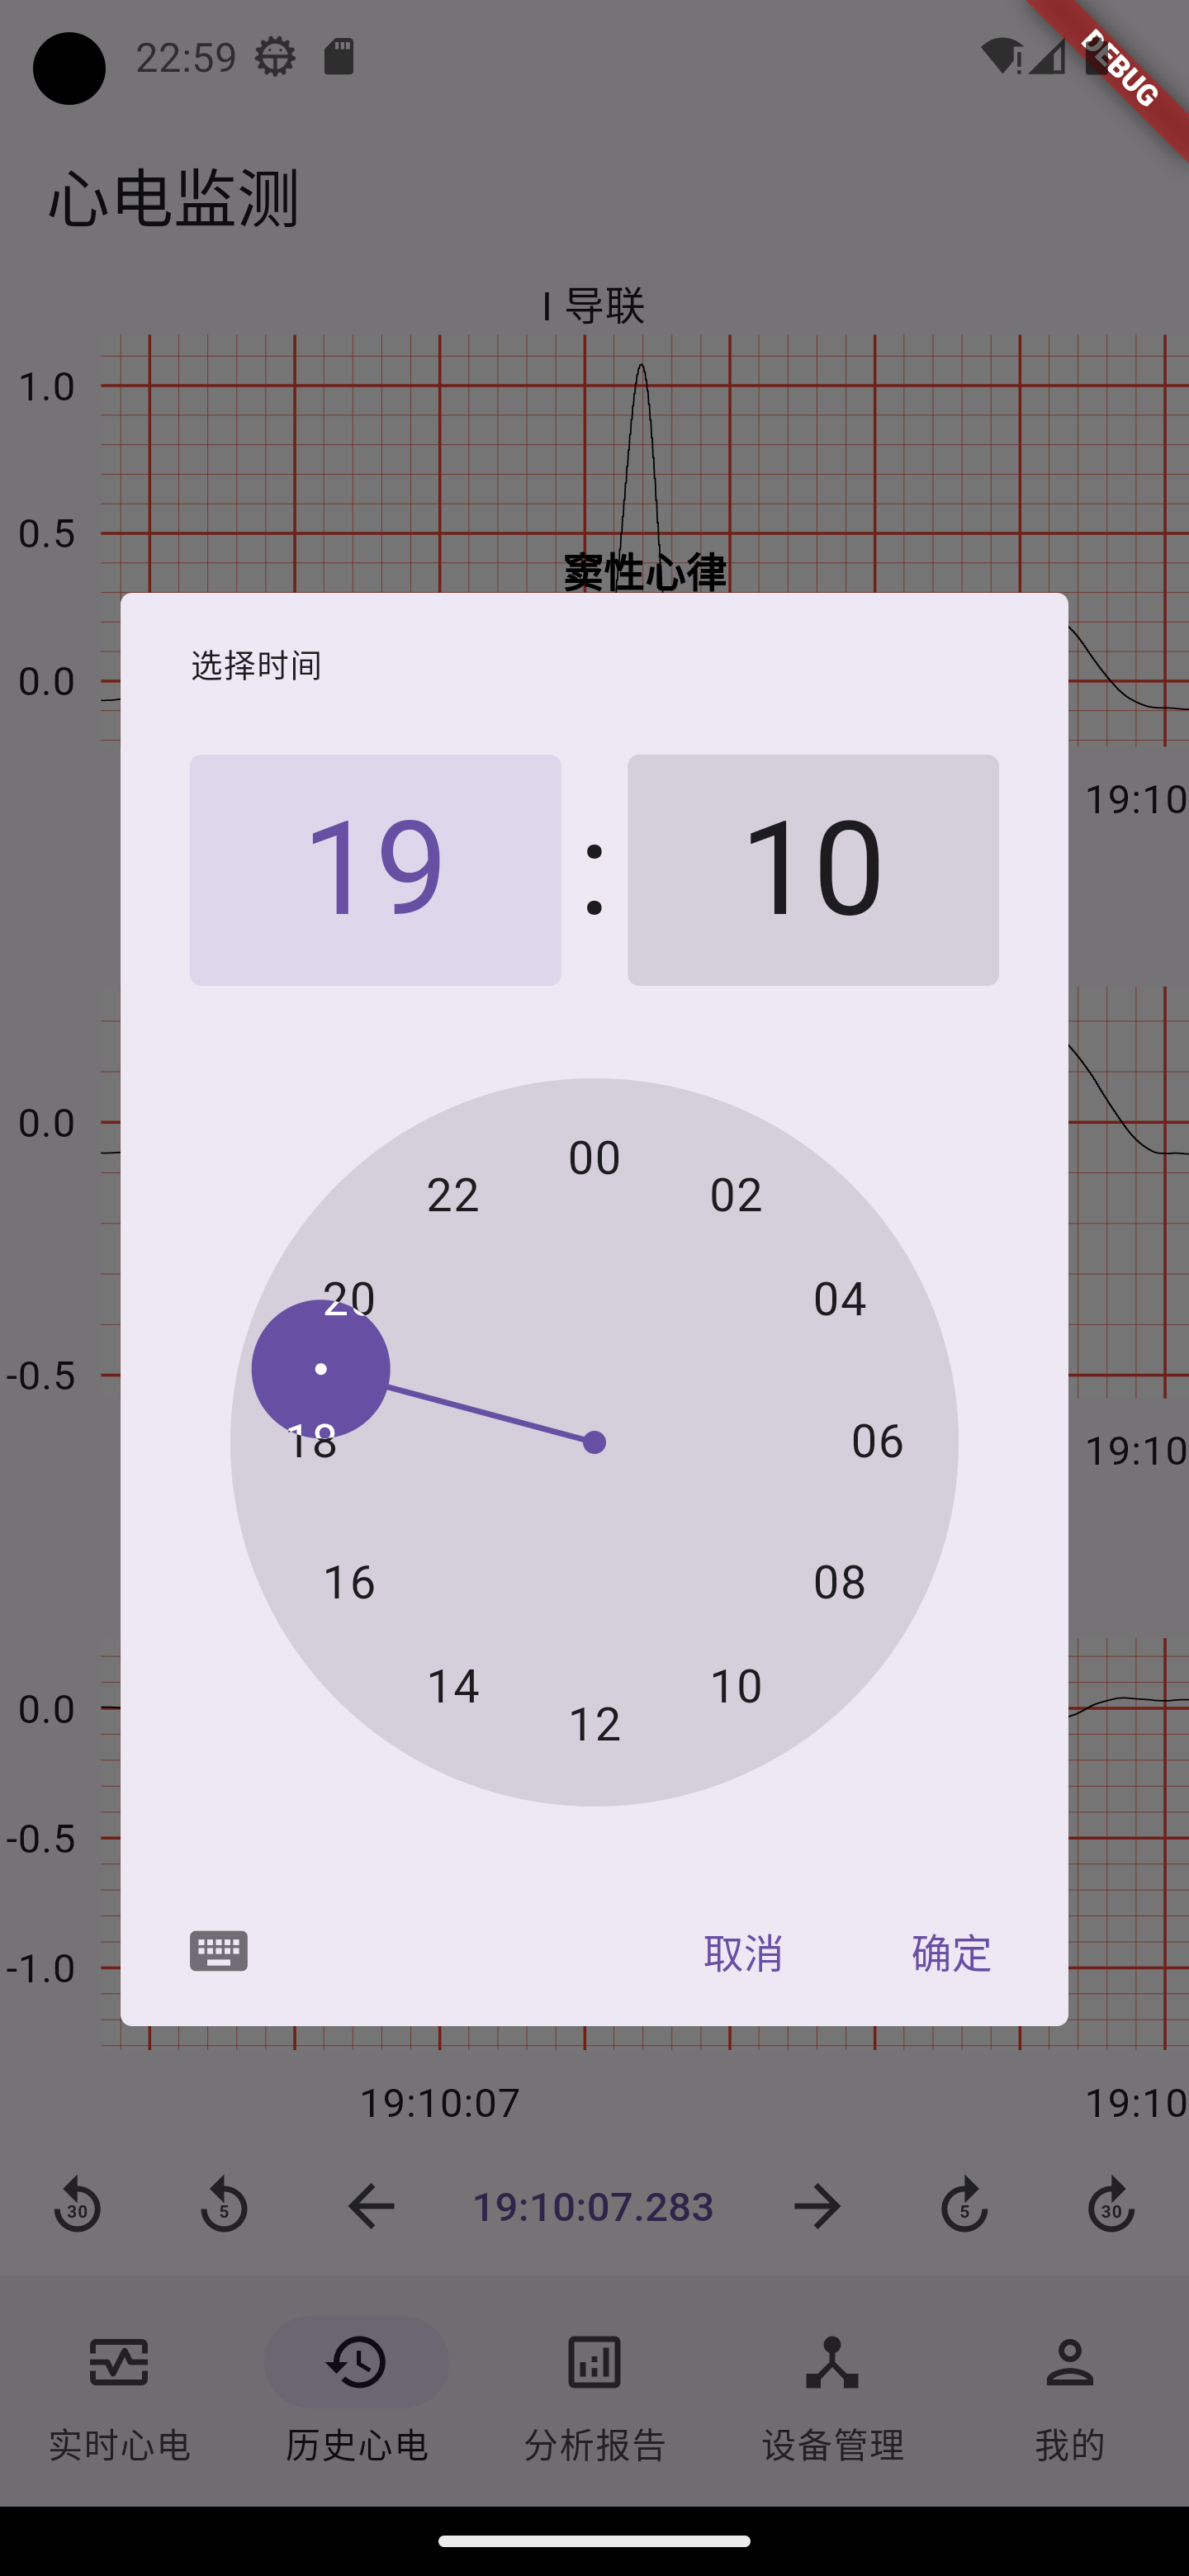
\includegraphics[width=.33\textwidth]{../assets/history-dialog-clock}}
    \subcaptionbox{数字模式输入}{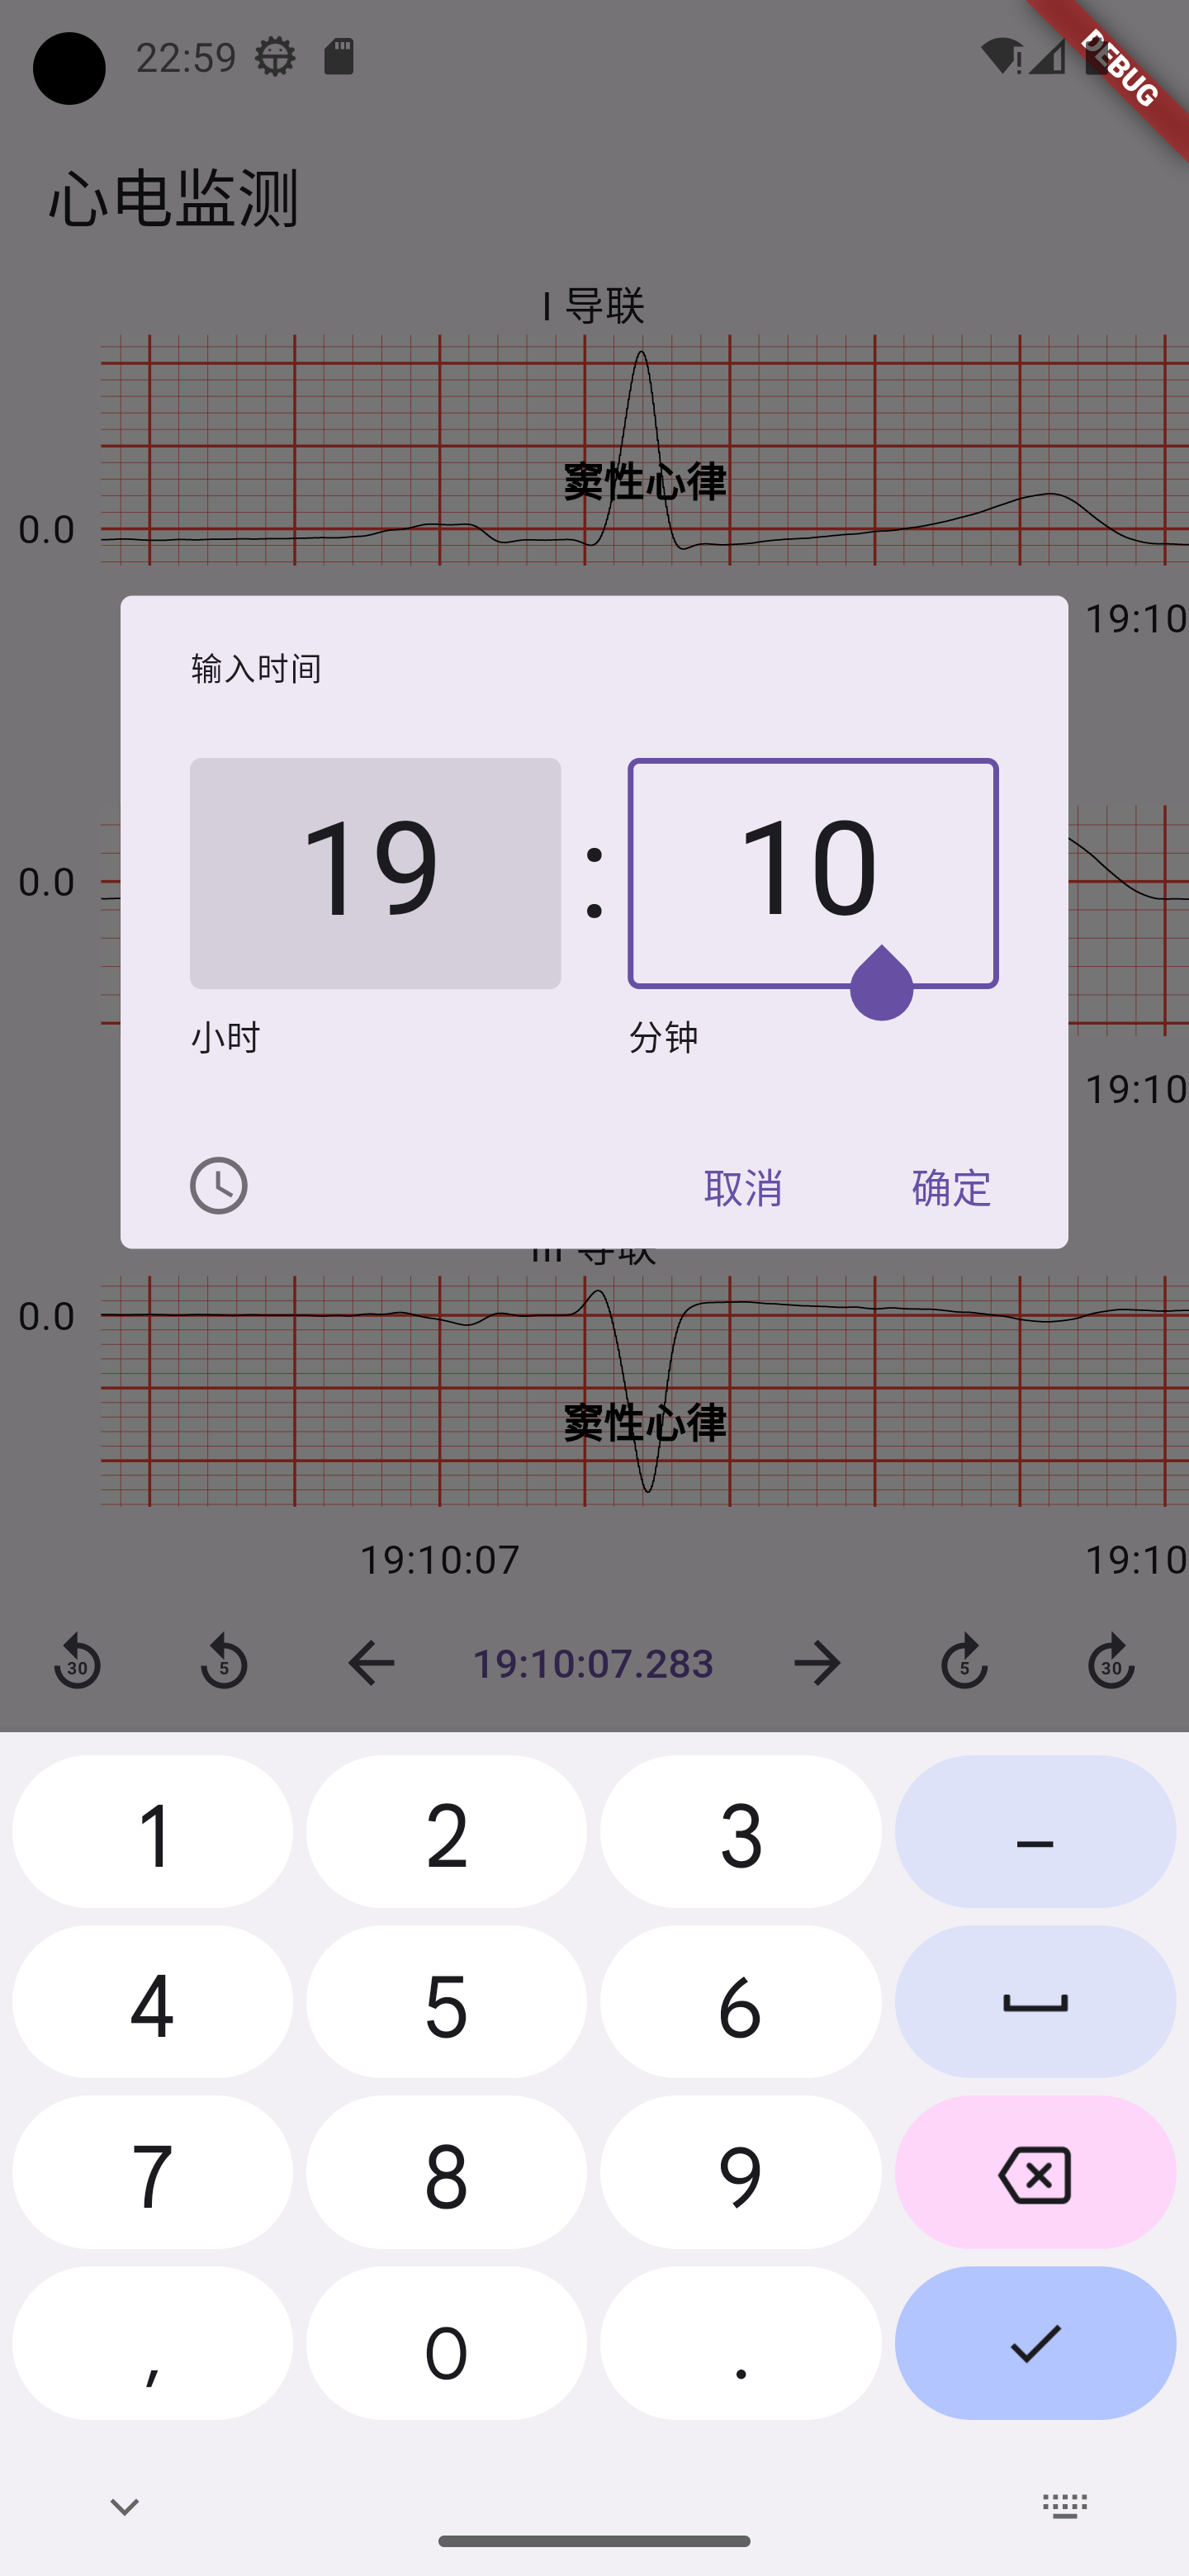
\includegraphics[width=.33\textwidth]{../assets/history-dialog-field}}
    \bicaption{历史心电时间选择器的截图}{Screenshot of the history ECG time picker}
    \label{fig:history-time-picker}
\end{figure}

从图中也可以看出,当可用显示区域由于键盘的弹出而缩小时,应用的界面布局仍然可以保持基本可用。这也体现了应用的界面可以适应不同尺寸、不同屏幕比例的设备,并且对分屏等比例特殊的情况也有支持。

\todo{心电模块的更多实现细节}


\section{分析报告模块的实现}\label{sec:analytics}

\subsection{分析报告界面的实现}\label{subsec:analytics-ui}

分析报告界面的整体外观如图~\ref{fig:analytics} 所示。在导航栏中为分析报告使用了表示数据分析的图标。

\begin{figure}[ht]
    \subcaptionbox{加载中}{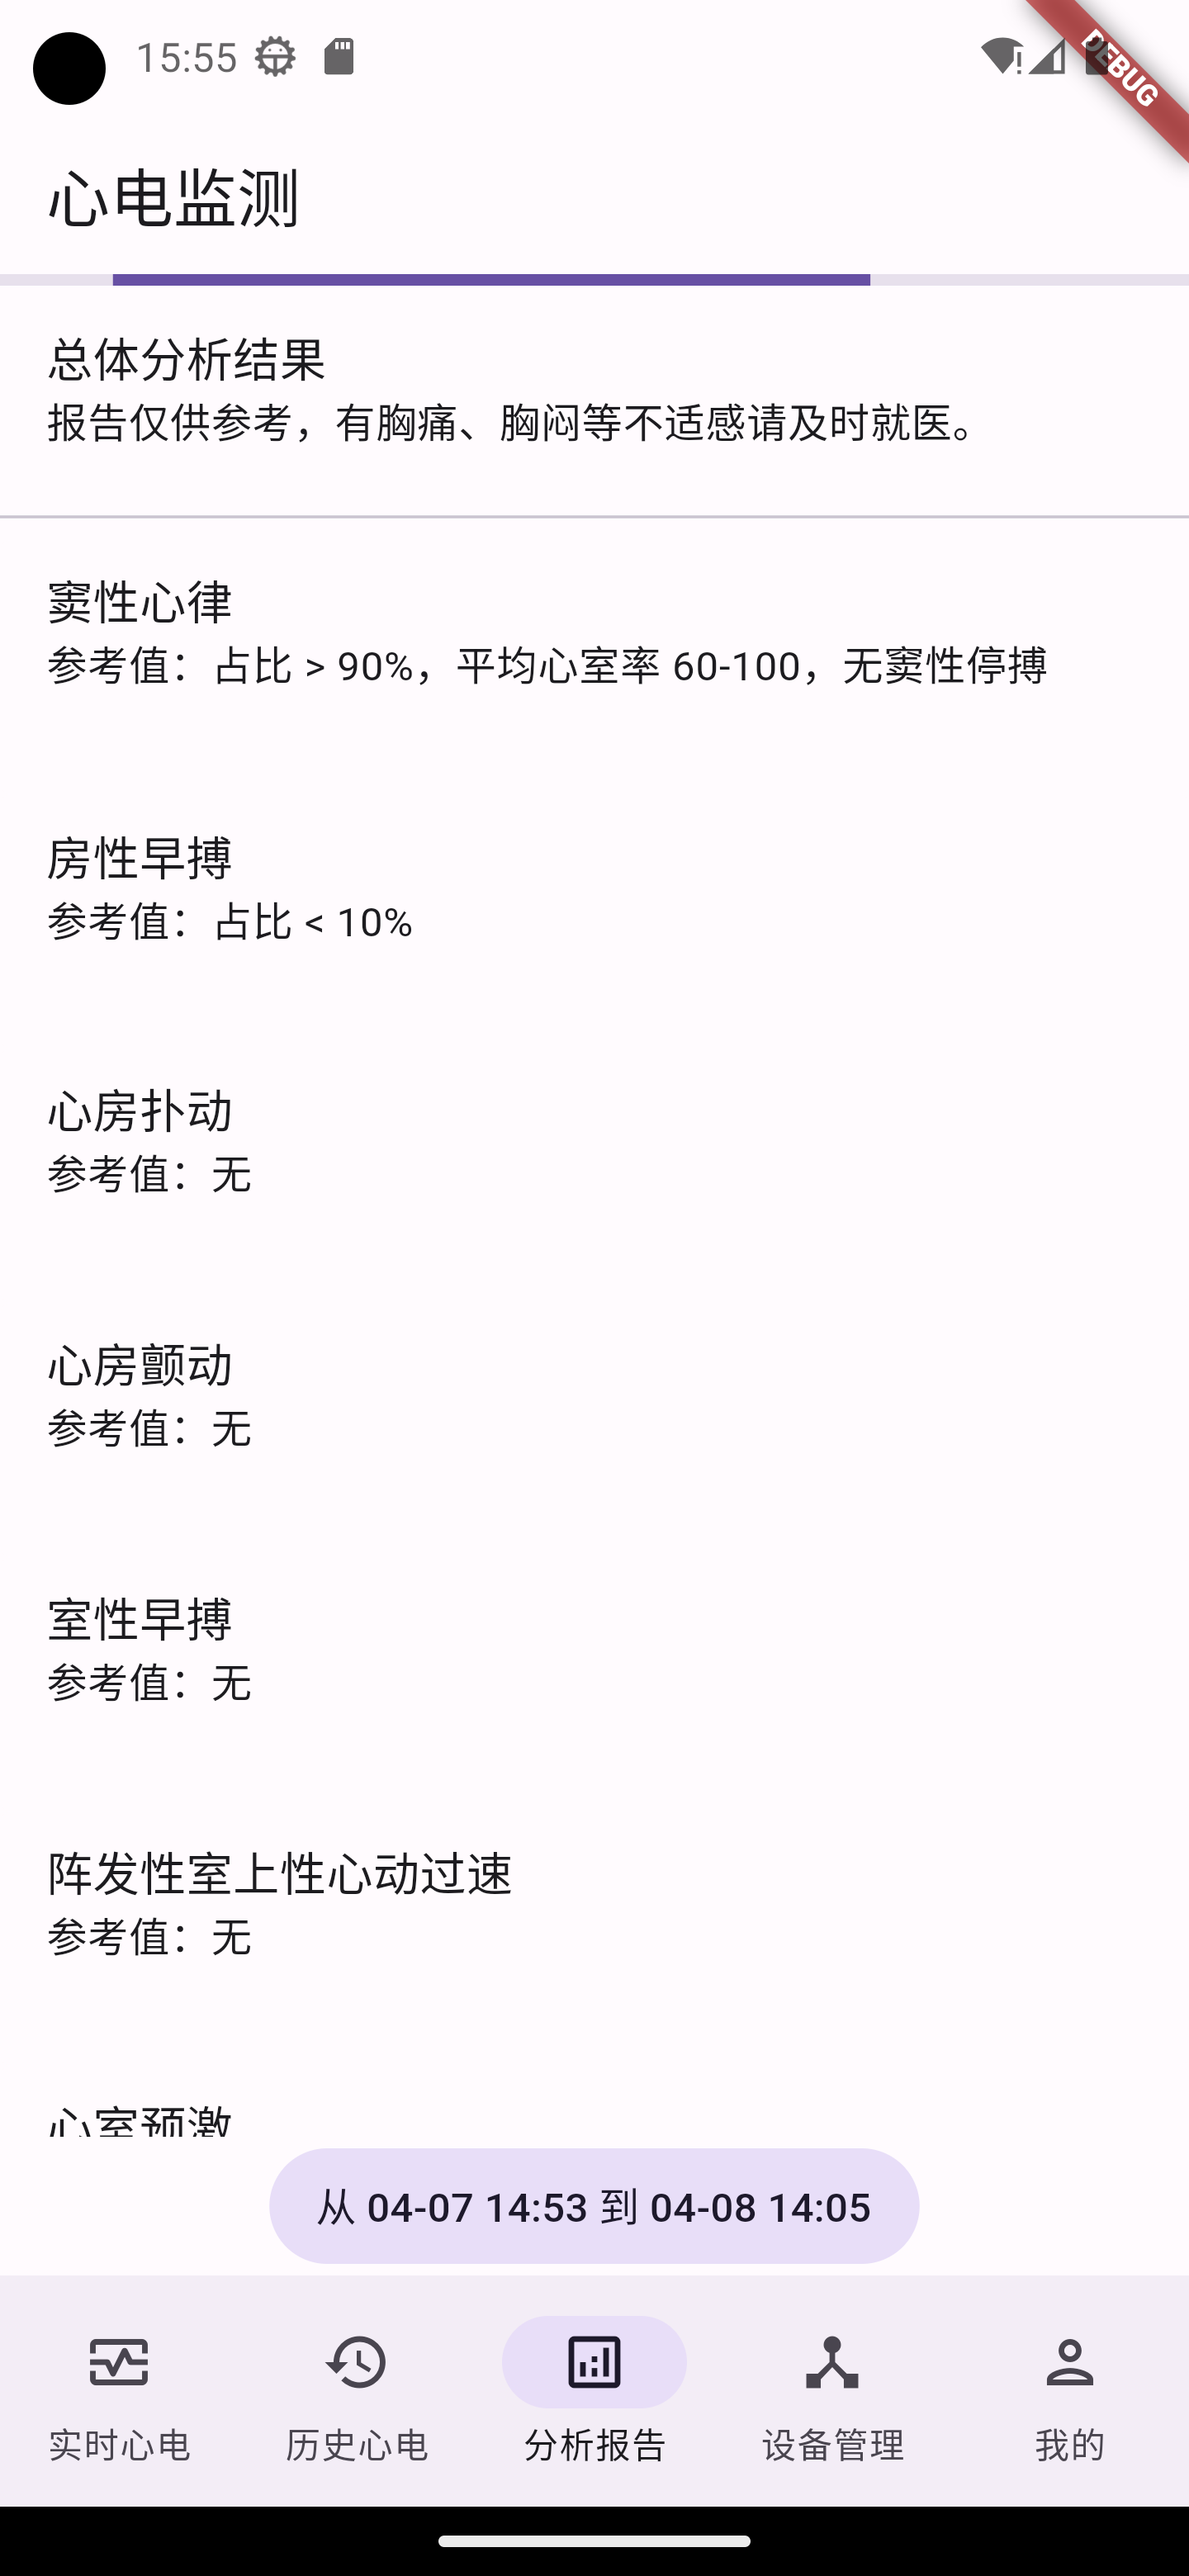
\includegraphics[width=.33\textwidth]{../assets/analytics-loading}}
    \subcaptionbox{正常状态}{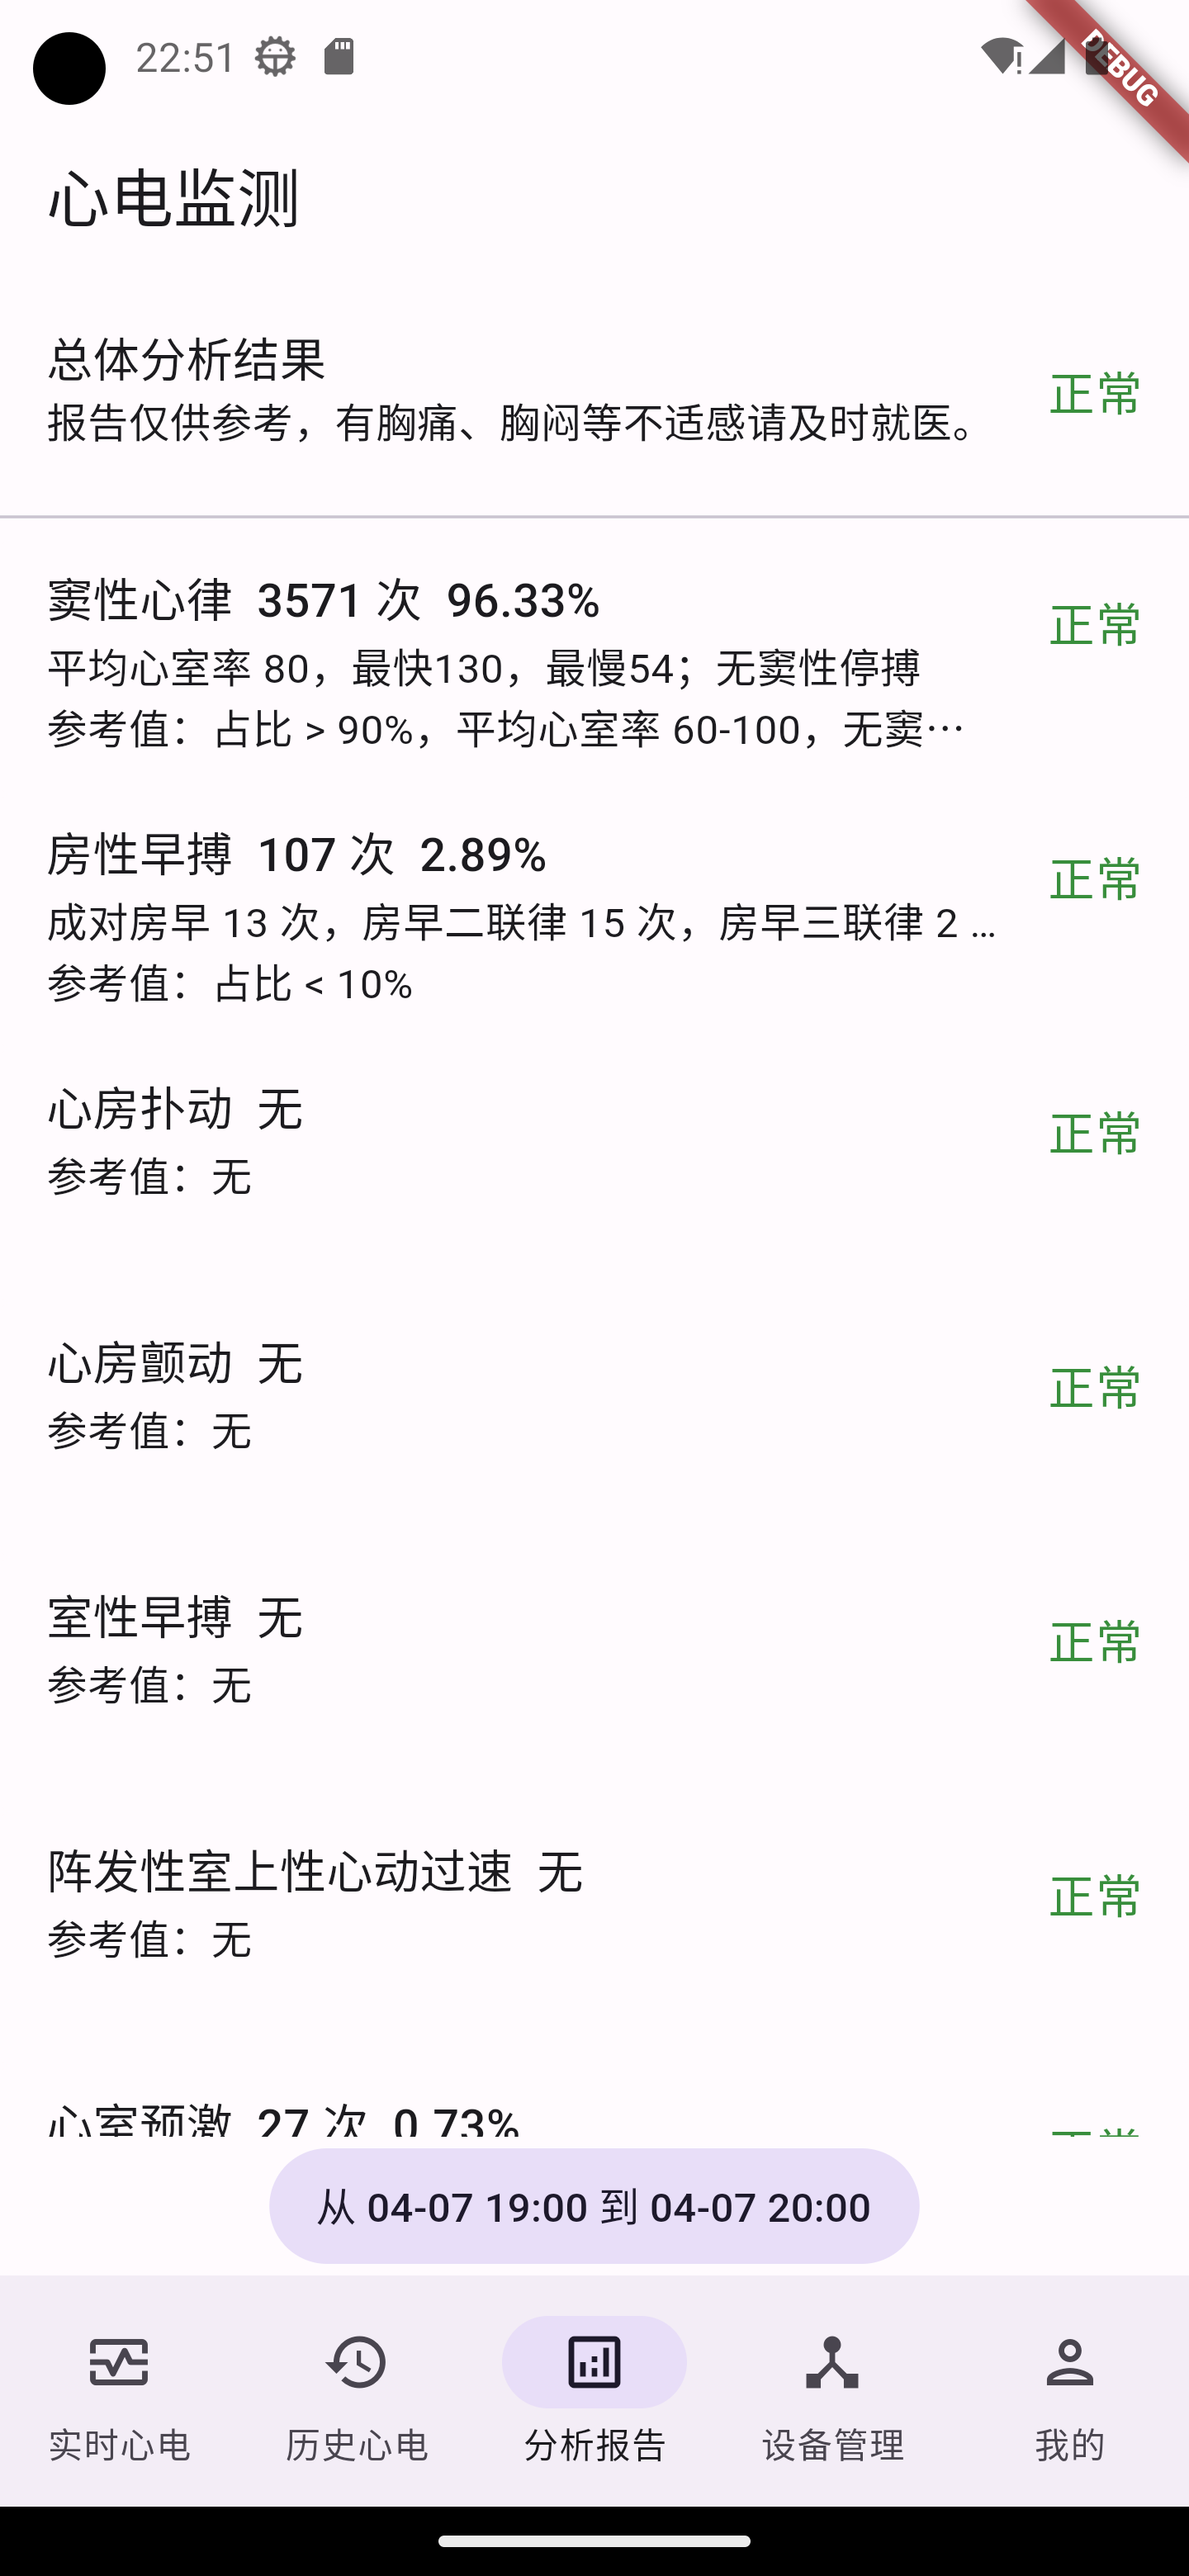
\includegraphics[width=.33\textwidth]{../assets/analytics}}
    \subcaptionbox{时间范围选择}{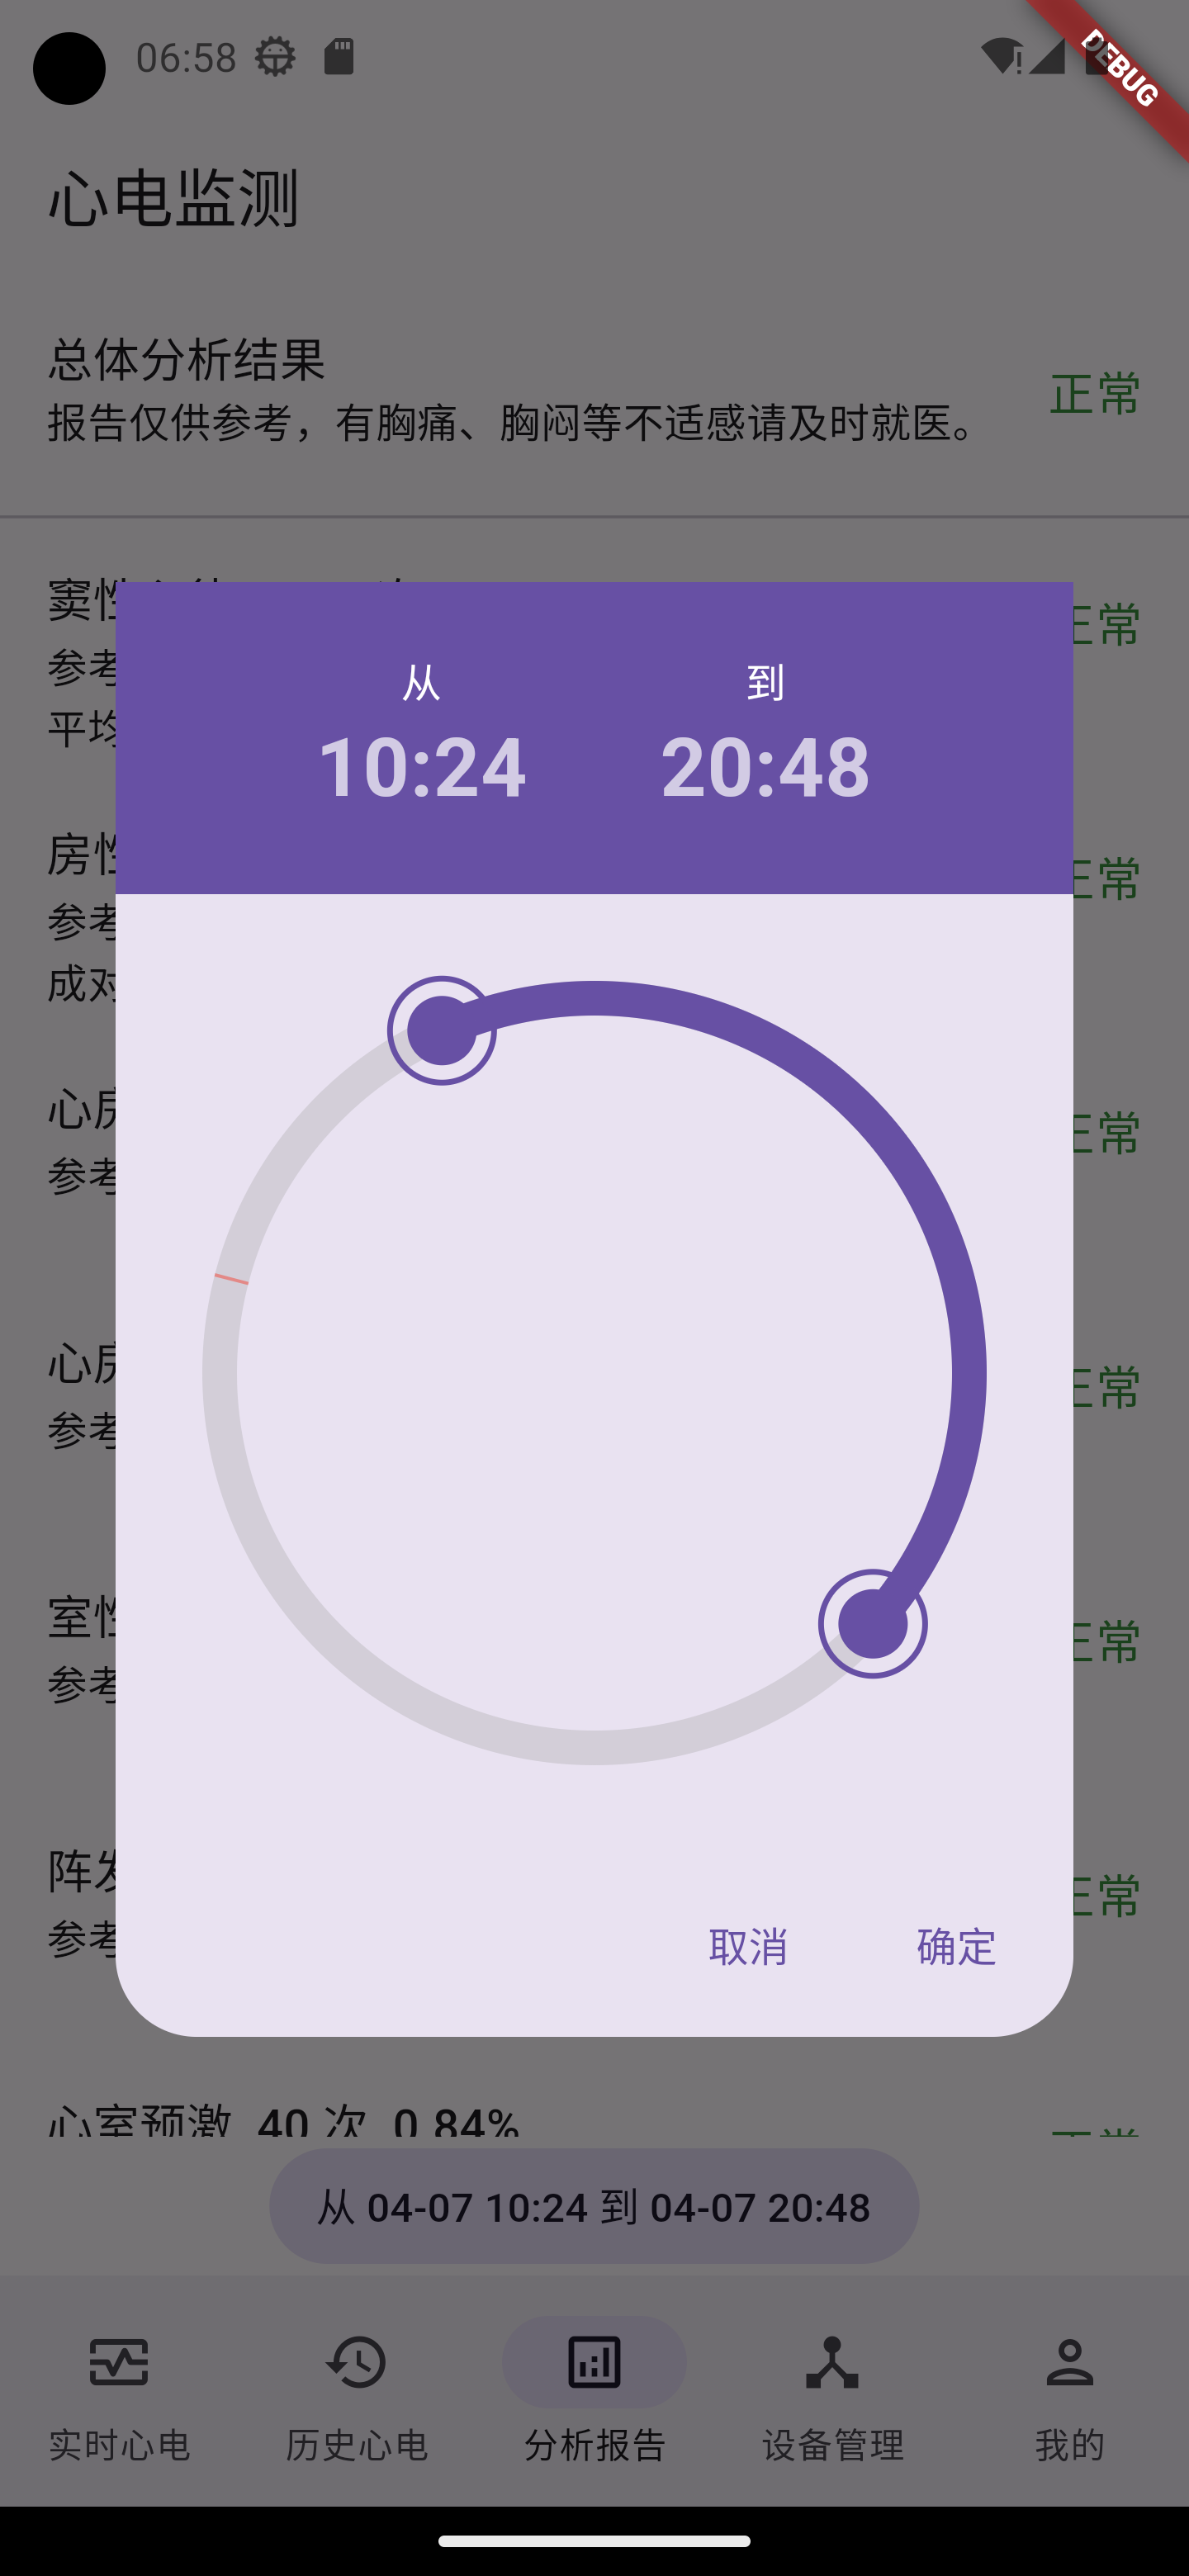
\includegraphics[width=.33\textwidth]{../assets/analytics-dialog}}
    \bicaption{分析报告界面的截图}{Screenshot of the analytics page}
    \label{fig:analytics}
\end{figure}

该界面可以划分为分析报告展示与时间范围选择器两部分,另外点击心律类型可以展开心律类型详情界面。

\subsubsection{分析报告展示部分的界面实现}\label{subsubsec:analytics-display-ui}

该部分区域整体上是一个可以上下滑动的列表。由于分析报告内容过多,在一个屏幕内完全展示会过于拥挤,所以使用了可滑动列表的形式。

最上方的一小条区域是线状进度指示器。由于难以确定生成分析报告所需的具体时长,所以该进度指示器是不确定进度的样式。另外,由于该部分有很多界面元素可以在获取到实际数据之前就确认其内容与位置,所以没有像历史心电界面那样使用屏幕中央的圆形加载进度指示器,而只是在最上方使用了线状进度指示器,并在加载时提前显示部分可以确定的元素,以减少加载前后的界面变化,提升用户对界面内容的确定感。在加载完成后,该区域并不会直接消失,而是会替换为不可见的与进度指示器高度相同的空白元素,以保证界面布局的稳定性,避免下方内容在加载完成后突然上移。

在进度指示器之下显示了所选时间范围的分析结果的总结,以右侧以带颜色的字体显示对分析结果的简要概括(“正常”、“心动过速”等),并在下方给出稍详细一些的解释。

总结区域的下方放置了一条分割线,用以分割总体分析结果与具体的心律类型分析结果,并在视觉上对总体结果加以适当强调。

在分割线之下,每个心律类型的分析结果都会显示在一个独立的区域中。首先以稍大的字体显示心律类型的名称、次数、占比,然后以小一些的字体给出该心律类型相关数据的正常范围作为参考值,第三行显示部分心律类型会具有的额外信息,如成对房早次数等;后两行的内容各自被限制在一行之内,溢出的内容会被以省略号替代,以提示用户可以点击该区域查看更多信息。此外,每个心律类型的右侧也和总结一样给出了对该心律类型分析结果的简要概括。

各个心律类型的区域都是可以点击展开查看详细信息的。通常而言,可点击区域应当使用按钮等样式加以指示,但当屏幕上的可点击区域过多时应该避免过多的装饰,以免造成视觉上的混乱。对于列表项的可点击性的指示,一种常见的做法是在右侧显示一个箭头,但在本界面中右侧已经被占据,不便添加更多元素。因此,本界面使用了其他方式来提醒用户心律类型可以点击。除上文所述的省略号外,该界面利用下方被截断的列表项指示该区域可以滑动查看更多内容,并在用户滑过心律区域时展示了水墨扩散的效果,如图~\ref{fig:ink} 所示,效果会从点击位置向四周扩散。水墨扩散效果在Material设计中用于各种可点击区域的反馈,可以提醒用户心律展示区域点击后能触发额外动作。

\begin{figure}[ht]
    \centering
    
\includegraphics[width=.5\textwidth]{../assets/ink}
    \bicaption{心律类型区域的水墨扩散效果}{Ink effect of the heart rhythm area}
    \label{fig:ink}
\end{figure}

\subsubsection{时间范围选择器部分的界面实现}\label{subsubsec:analytics-time-range-ui}

时间范围选择器部分仅在中间包含一个填充色调按钮。因为需要明确提醒用户所示分析报告的时间范围,所以没有使用强调效果较弱的轮廓按钮和文本按钮。按钮中的文本指示了当前选择的时间范围。点击按钮后,会弹出时间范围选择对话框。

时间范围选择对话框的主体是一个圆环,用户可以拖动圆环上的两个点来选定分析范围的起止时间。为了不引起日期的混淆,当前时间(在圆环上显示为红色)不被允许包含在选择部分之中,这样可以保证用户所选的时间范围总是可以解释为过去24小时之内的某个时间段。

\subsection{心律类型详情界面的实现}\label{subsec:label-details}

心律类型详情界面的整体外观的如图~\ref{fig:label-details} 所示。除上方的心律名称和返回按钮外,界面由可滑动查看的列表构成。列表内容包括该心律类型的说明文本,以及心律出现的具体时间。为了保证每个时间都可以较容易点击到,时间之间留有适当的间隔。点击时间后,会跳转至历史心电的对应时间。

\begin{figure}[ht]
    \centering
    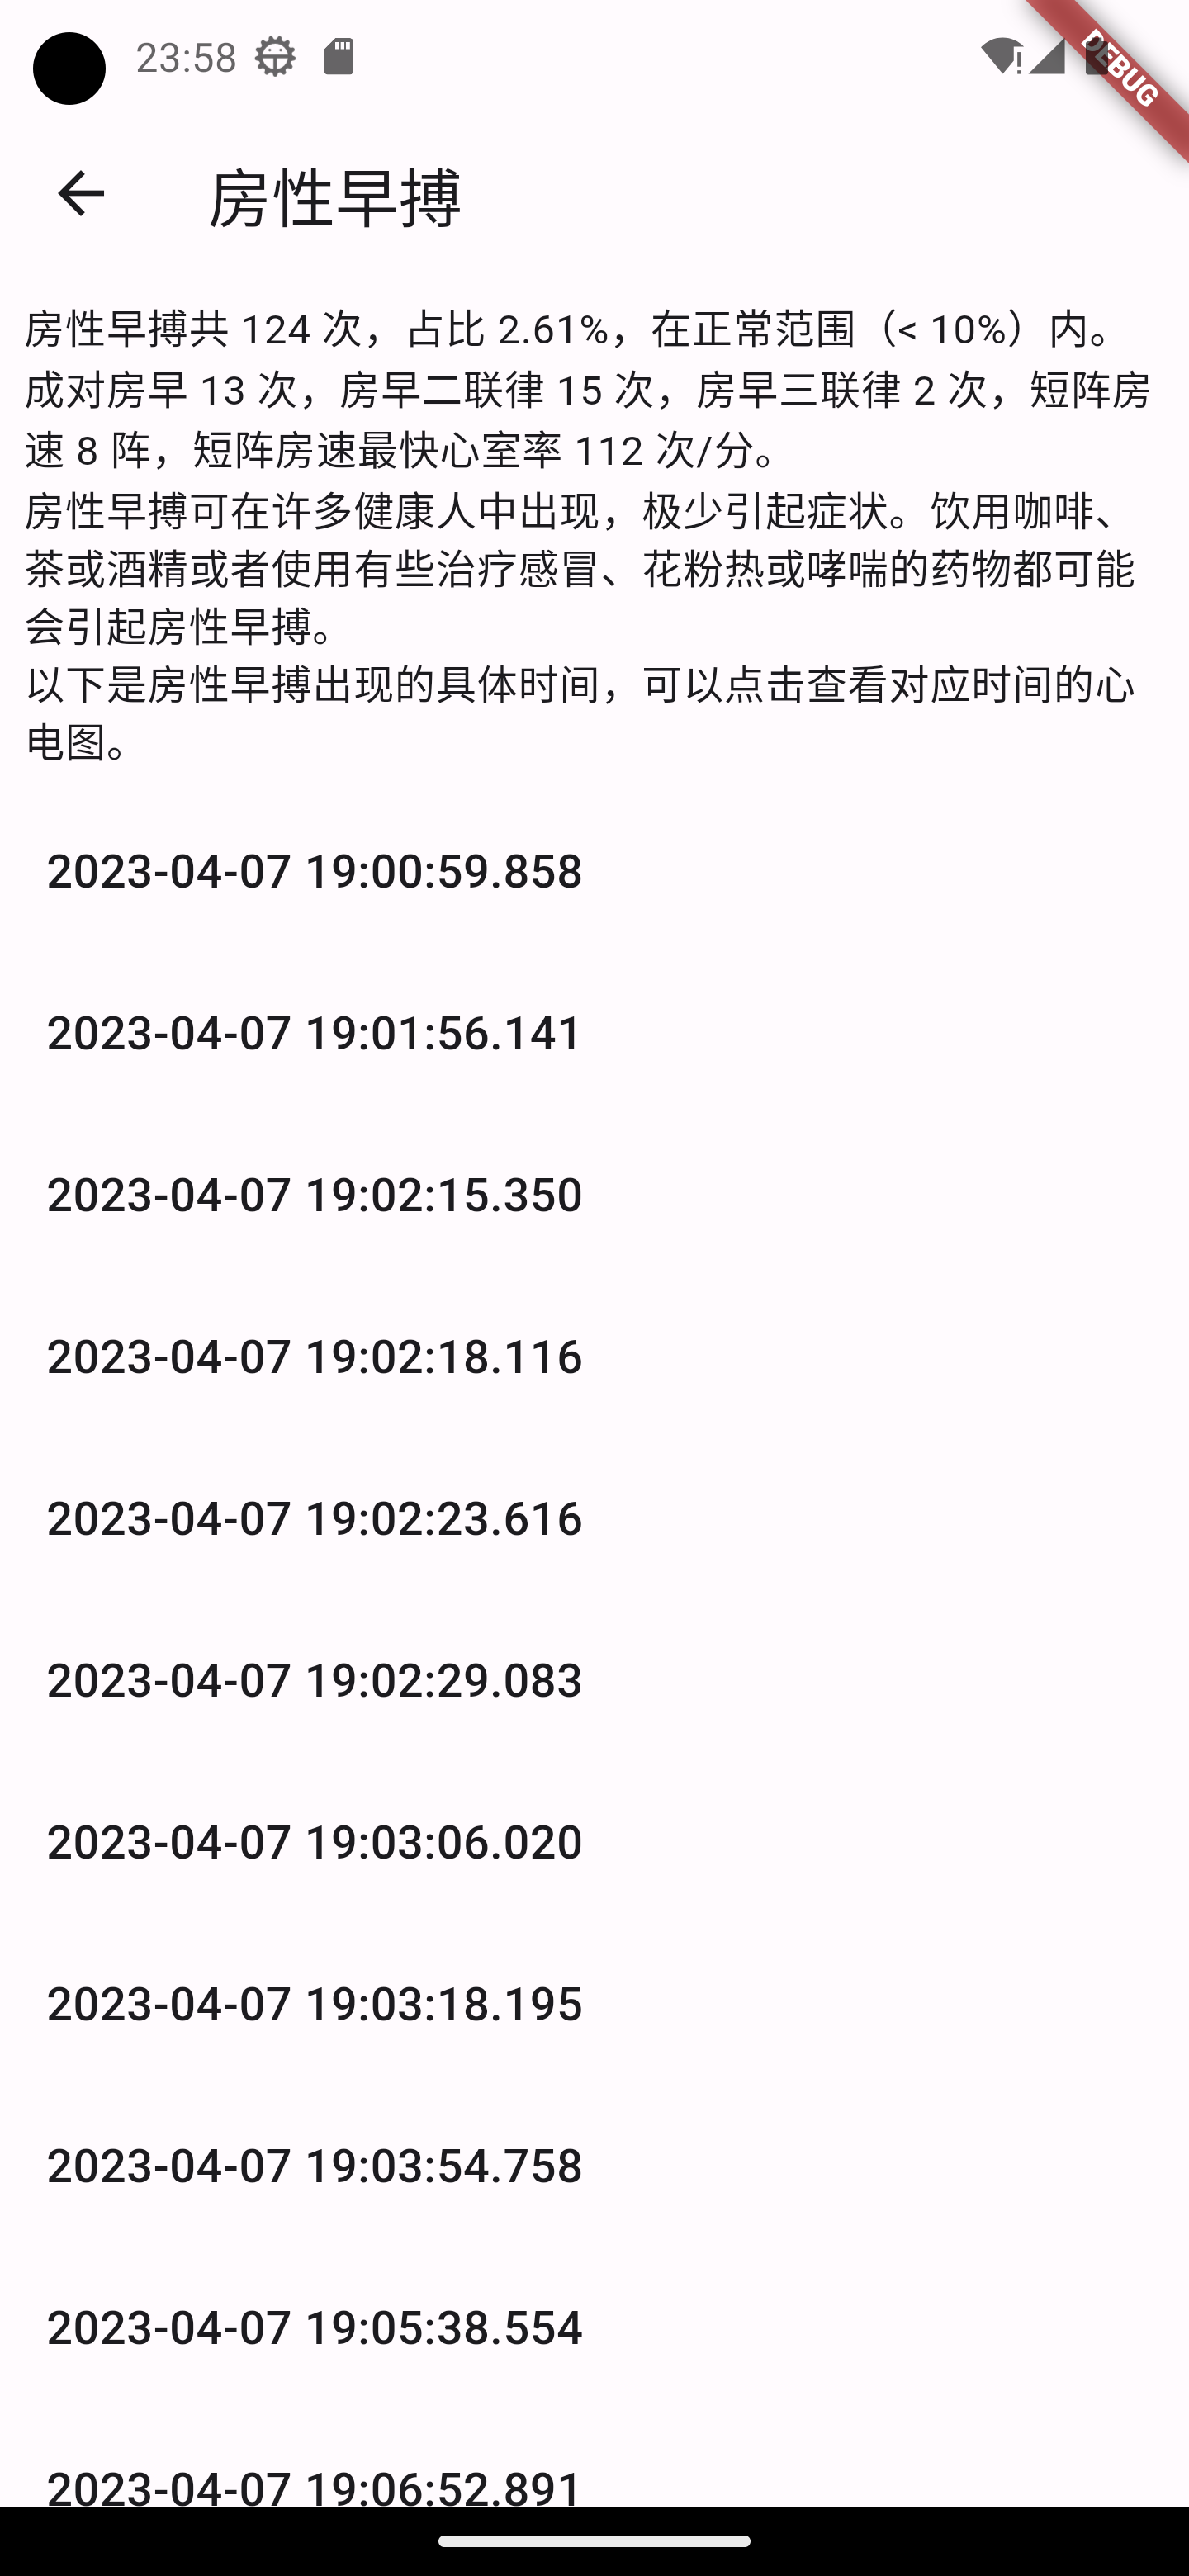
\includegraphics[width=.33\textwidth]{../assets/label-details}
    \bicaption{心律类型详情界面的截图}{Screenshot of the heart rhythm details page}
    \label{fig:label-details}
\end{figure}

\todo{分析报告模块的更多实现细节}


\section{设备管理模块的实现}\label{sec:device}

\subsection{设备管理界面的实现}\label{subsec:device-ui}

设备管理界面的整体外观如图~\ref{fig:device} 所示。设备管理在导航栏中的图标是对心电监测设备所使用的电极片的简化表示。

\begin{figure}[ht]
    \subcaptionbox{已连接}{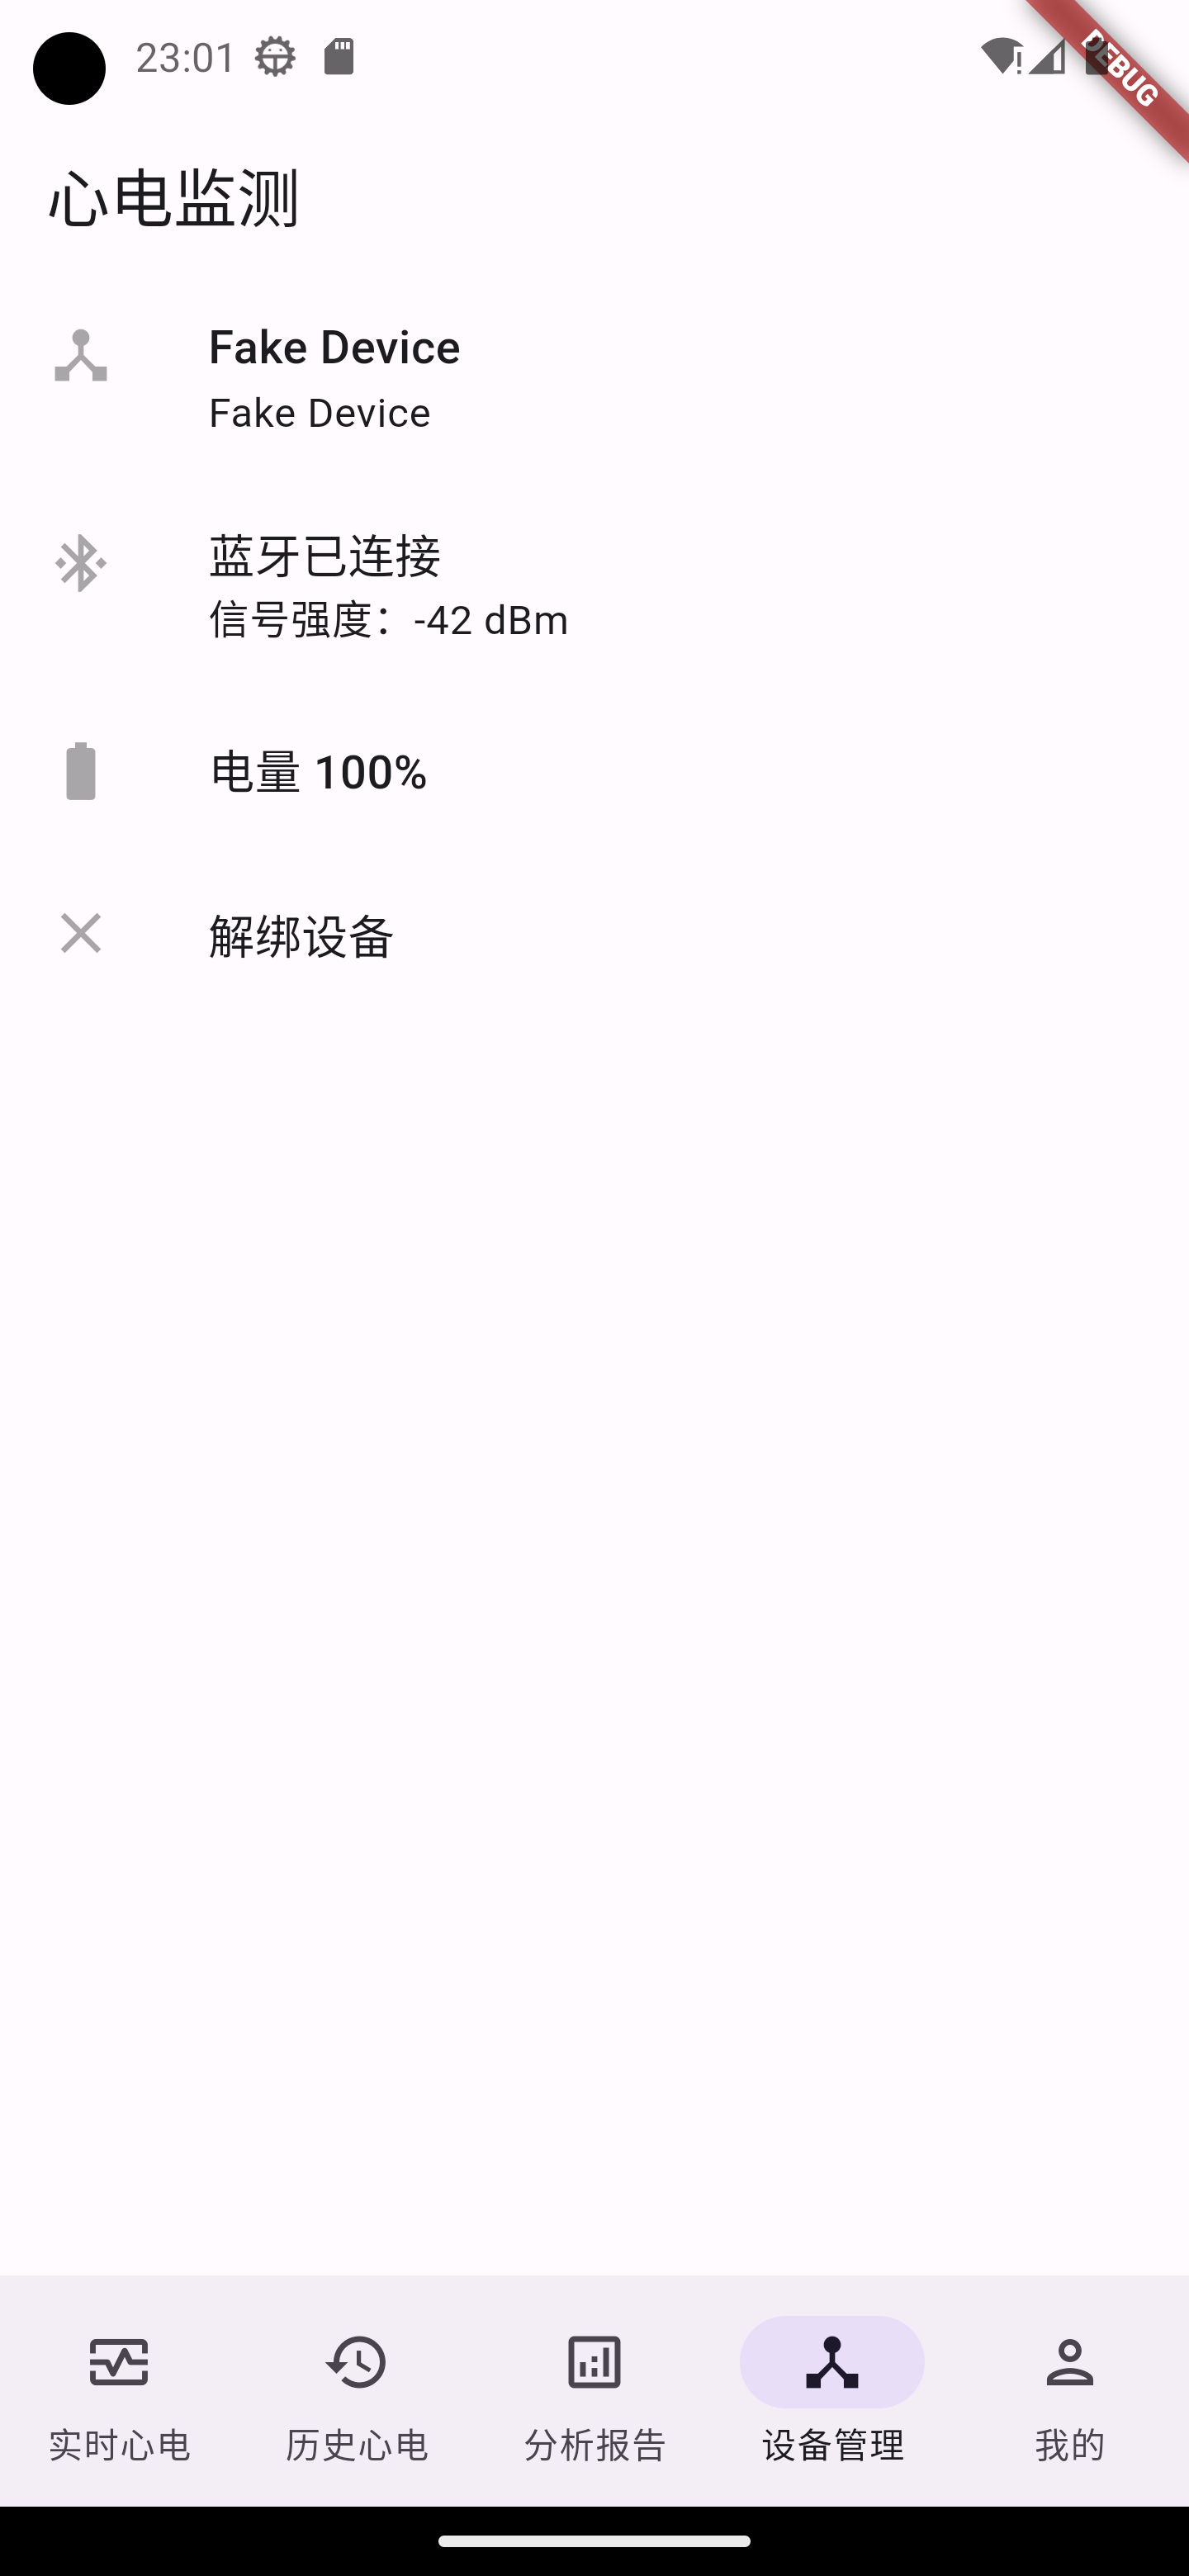
\includegraphics[width=.33\textwidth]{../assets/device-connected}}
    \subcaptionbox{连接新设备}{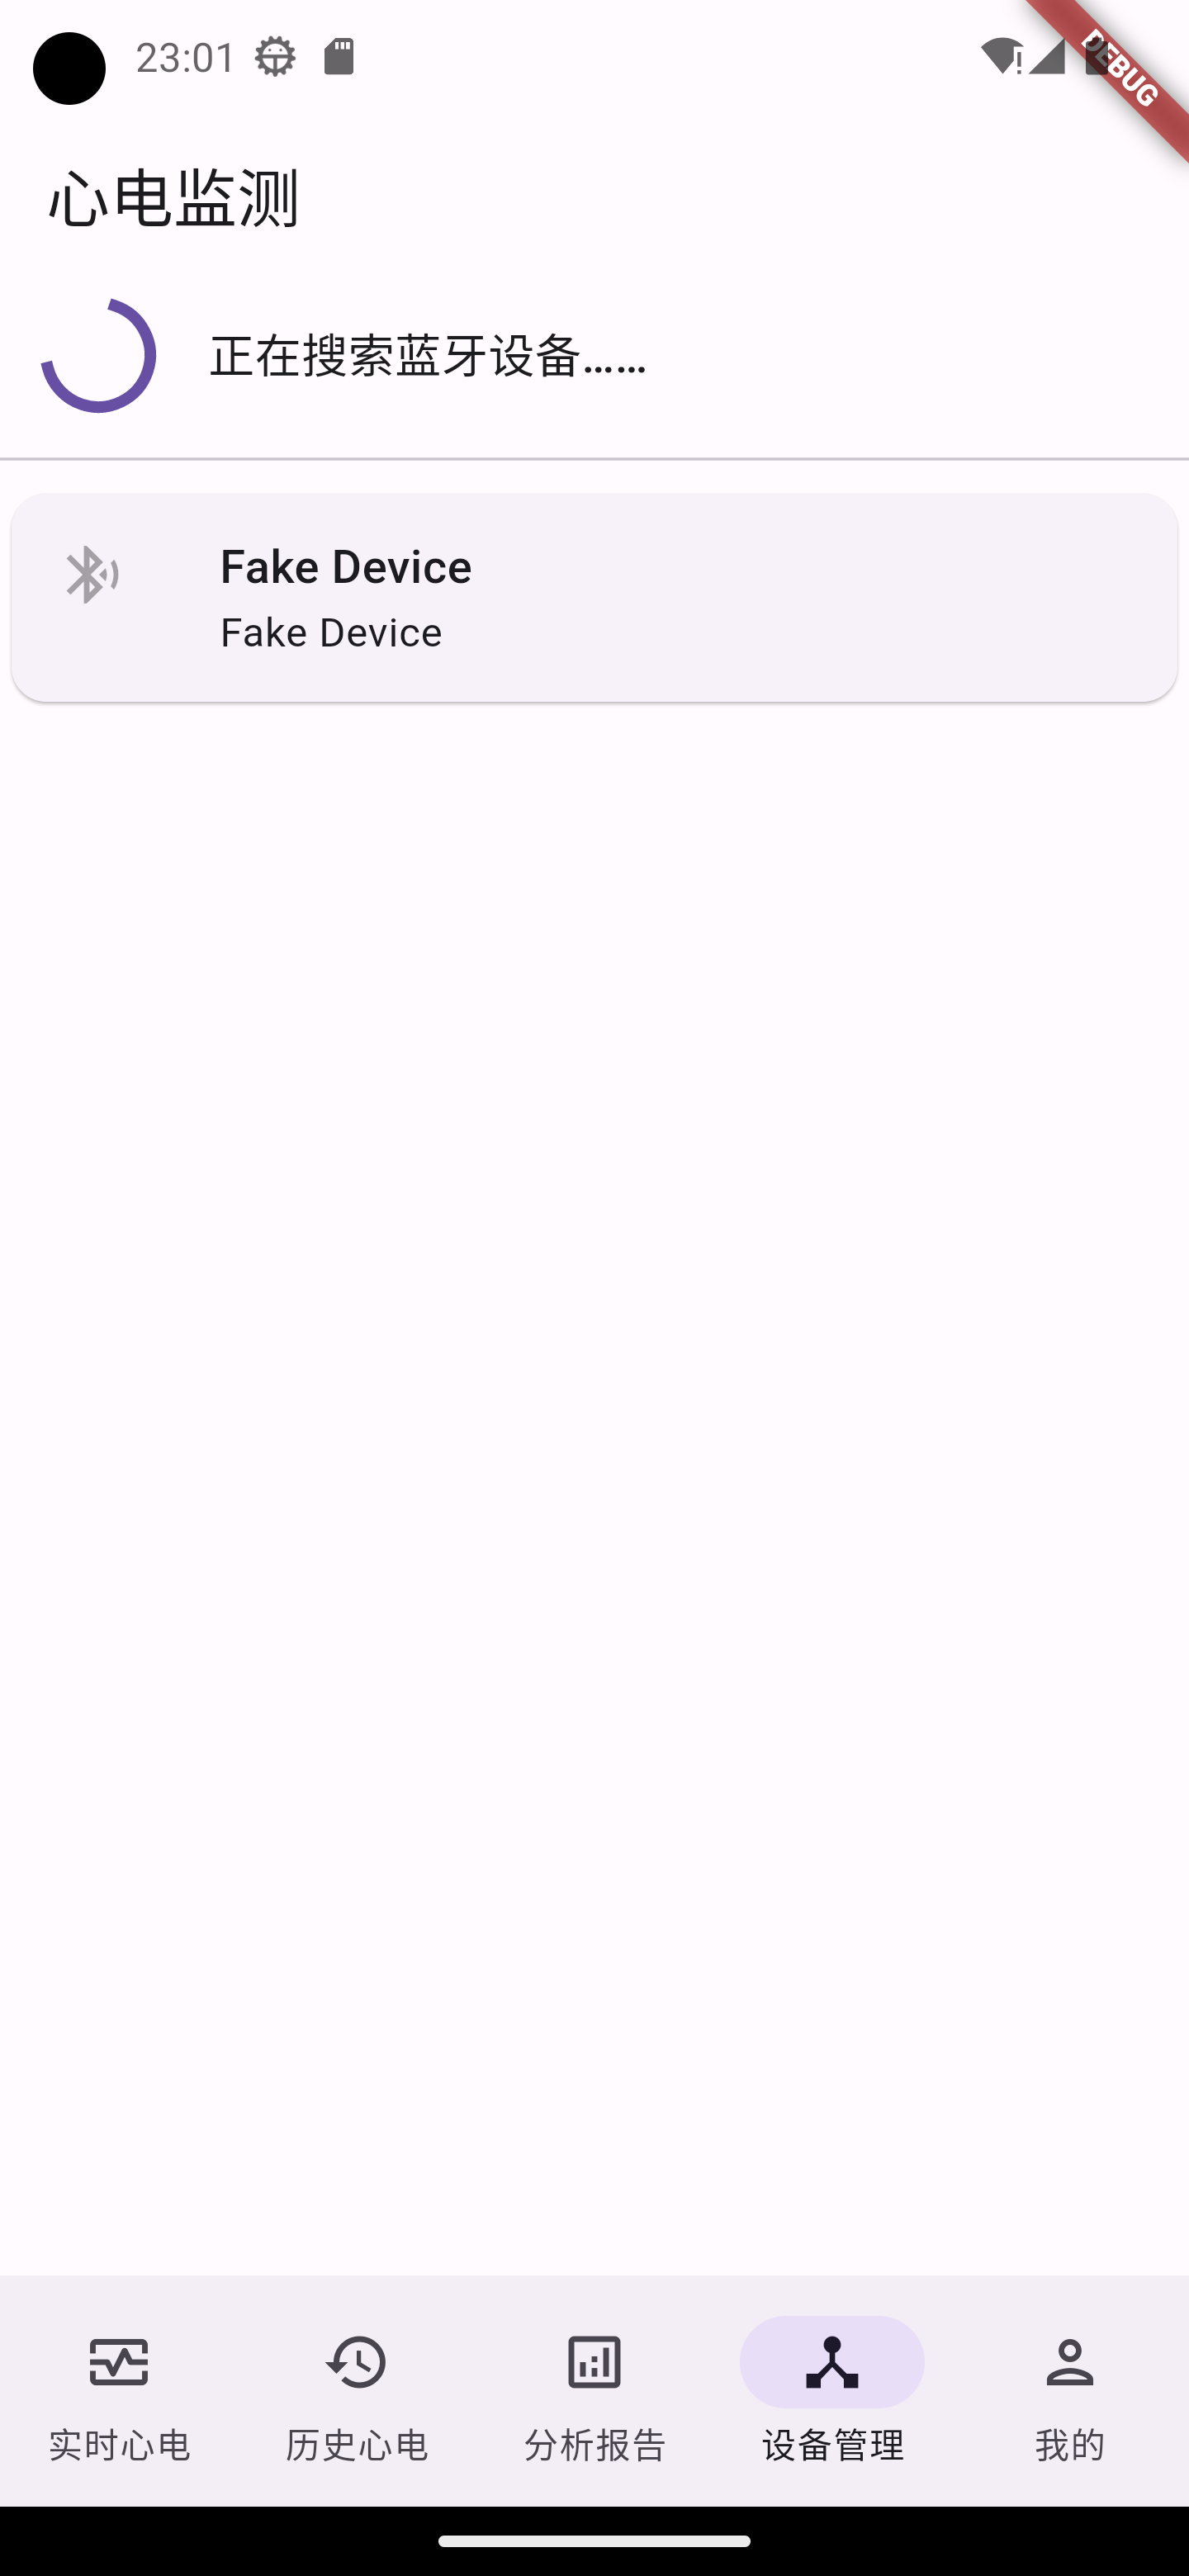
\includegraphics[width=.33\textwidth]{../assets/device-new}}
    \subcaptionbox{无可用设备}{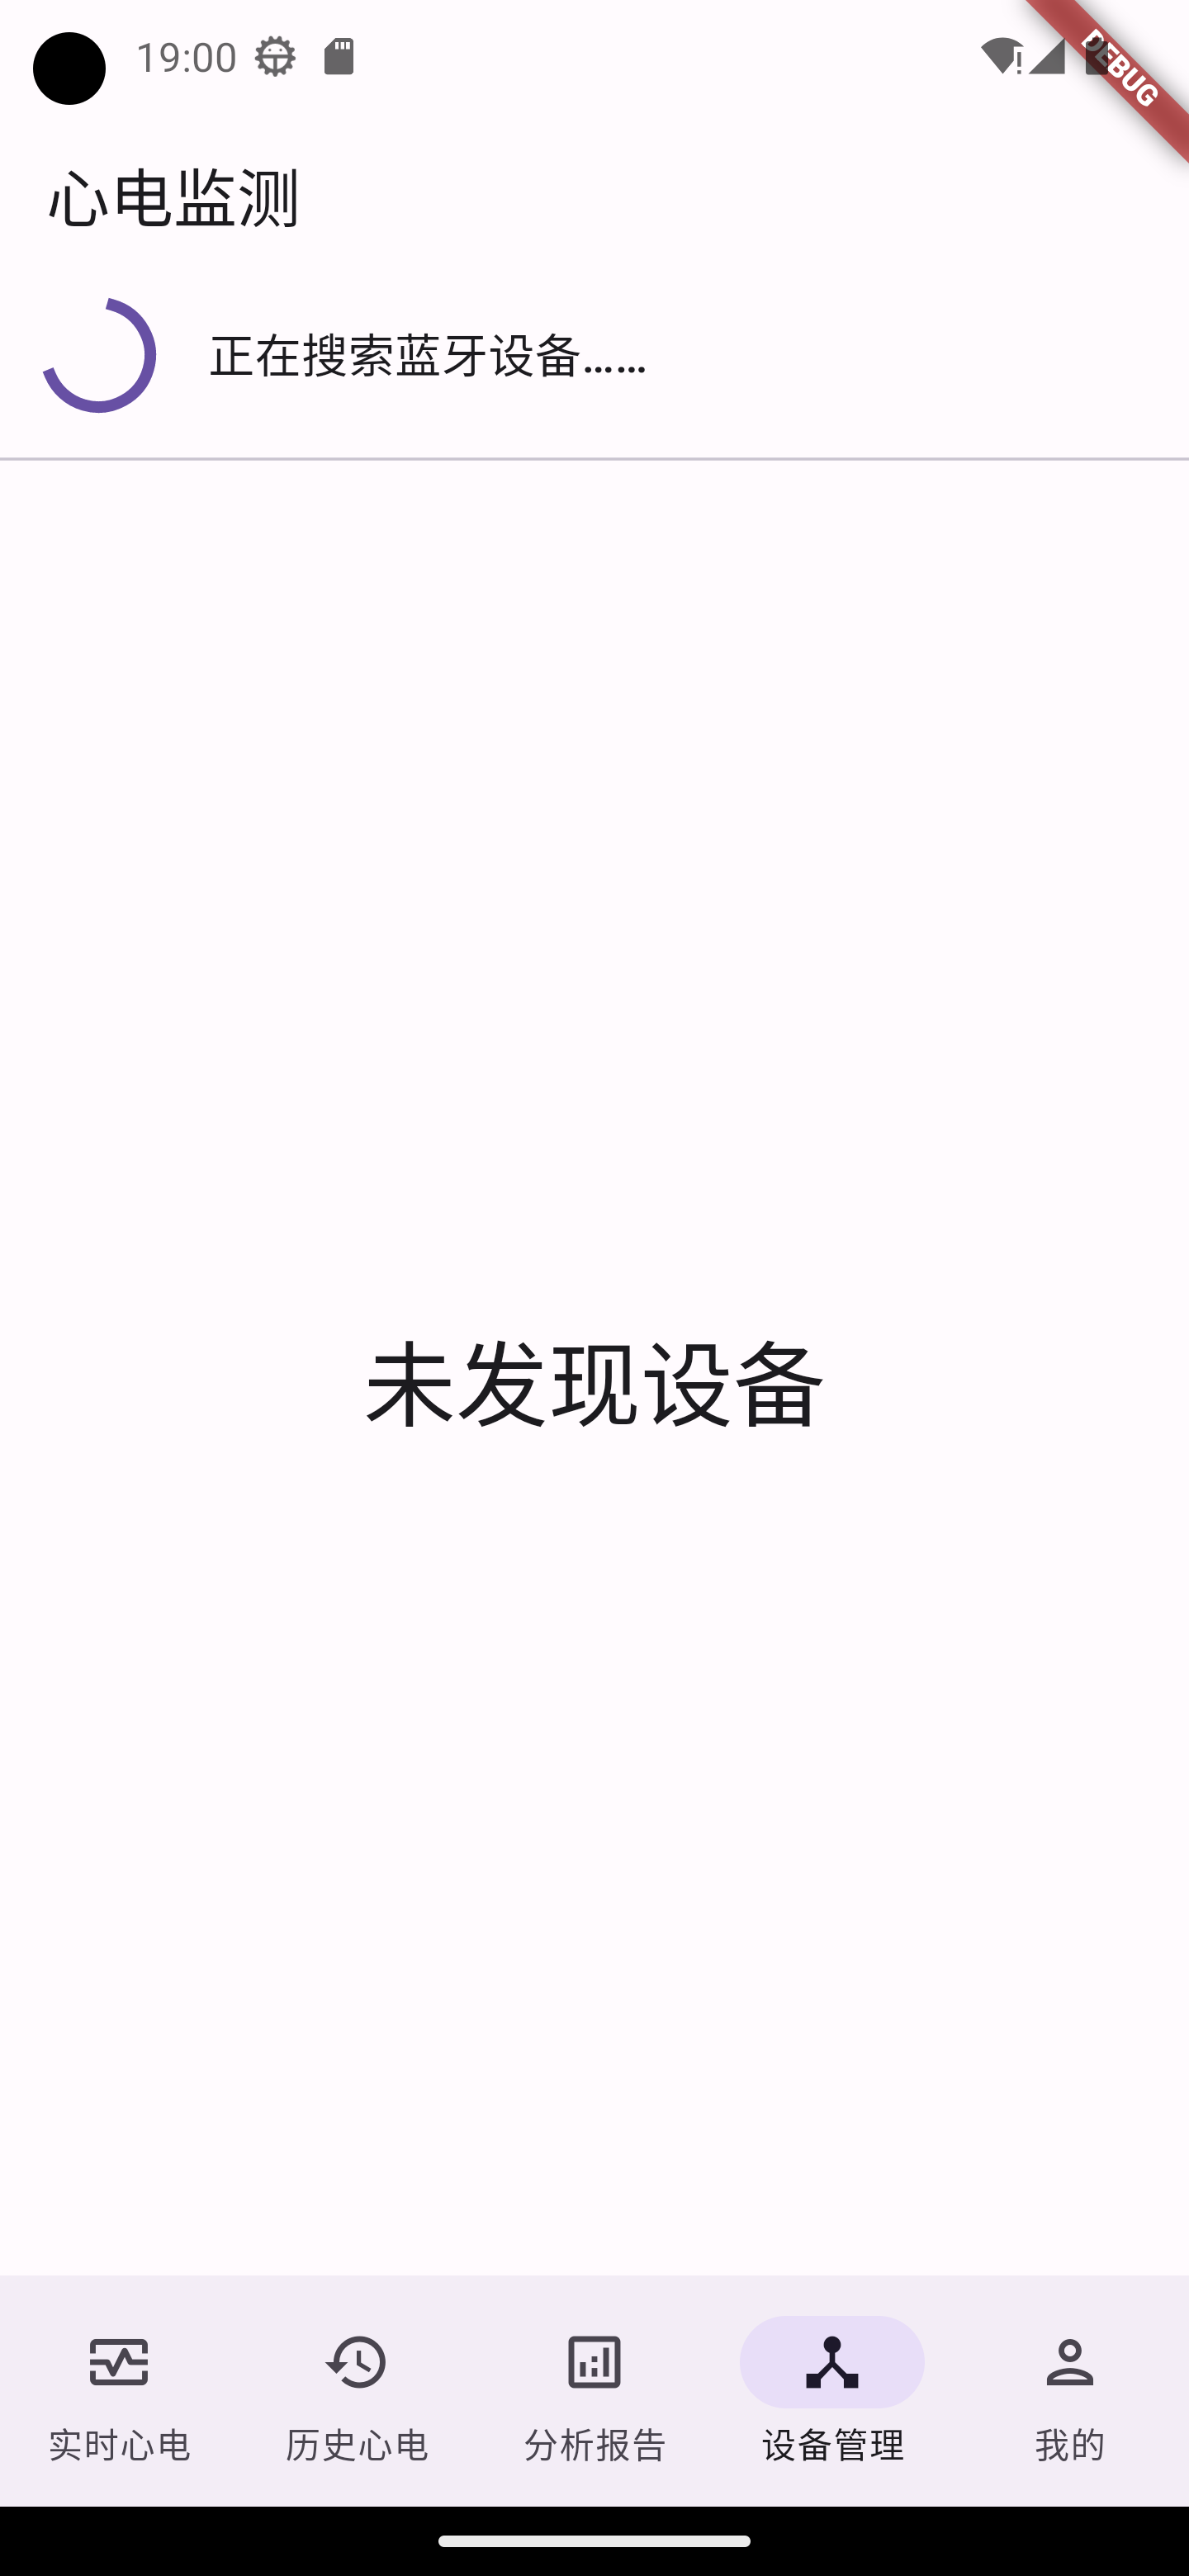
\includegraphics[width=.33\textwidth]{../assets/device-na}}
    \bicaption{设备管理界面的截图}{Screenshot of the device page}
    \label{fig:device}
\end{figure}

该界面相比上述其他界面较为简单,分为已绑定设备和未绑定设备两种状态。

在已绑定设备的状态下,该界面会以列表形式展示设备的名称、型号、信号强度、剩余电量与充电状态等信息,并提供解绑设备的按钮。该按钮没有使用额外的视觉效果来表示其可以点击,因为“解绑设备”这一文本本身已经足够明确地指示了该区域是可以点击的。

在未绑定设备的状态下,该界面会起到搜索并绑定设备的作用。界面上方展示“正在搜索蓝牙设备”的提示并显示了不确定进度的圆形进度指示器,之后有一条分割线,下方则展示了搜索到的设备列表。列表中的每一项都表示了一个搜索到的蓝牙设备(由于Android和iOS模拟器均不支持蓝牙功能,截图中仅显示了一个模拟设备),并以带阴影的卡片的样式来显示其可以直接点击,而没有额外放置绑定按钮,以使应用界面更加简洁。

\todo{设备管理模块的更多实现细节}


\section{其他功能的实现}\label{sec:other}

应用中包含一些不直接面向用户的辅助功能,或者虽然用户不常主动使用但仍然应该提供的功能,一些相关界面的外观如图~\ref{fig:other} 所示。

\begin{figure}[ht]
    \subcaptionbox{我的}{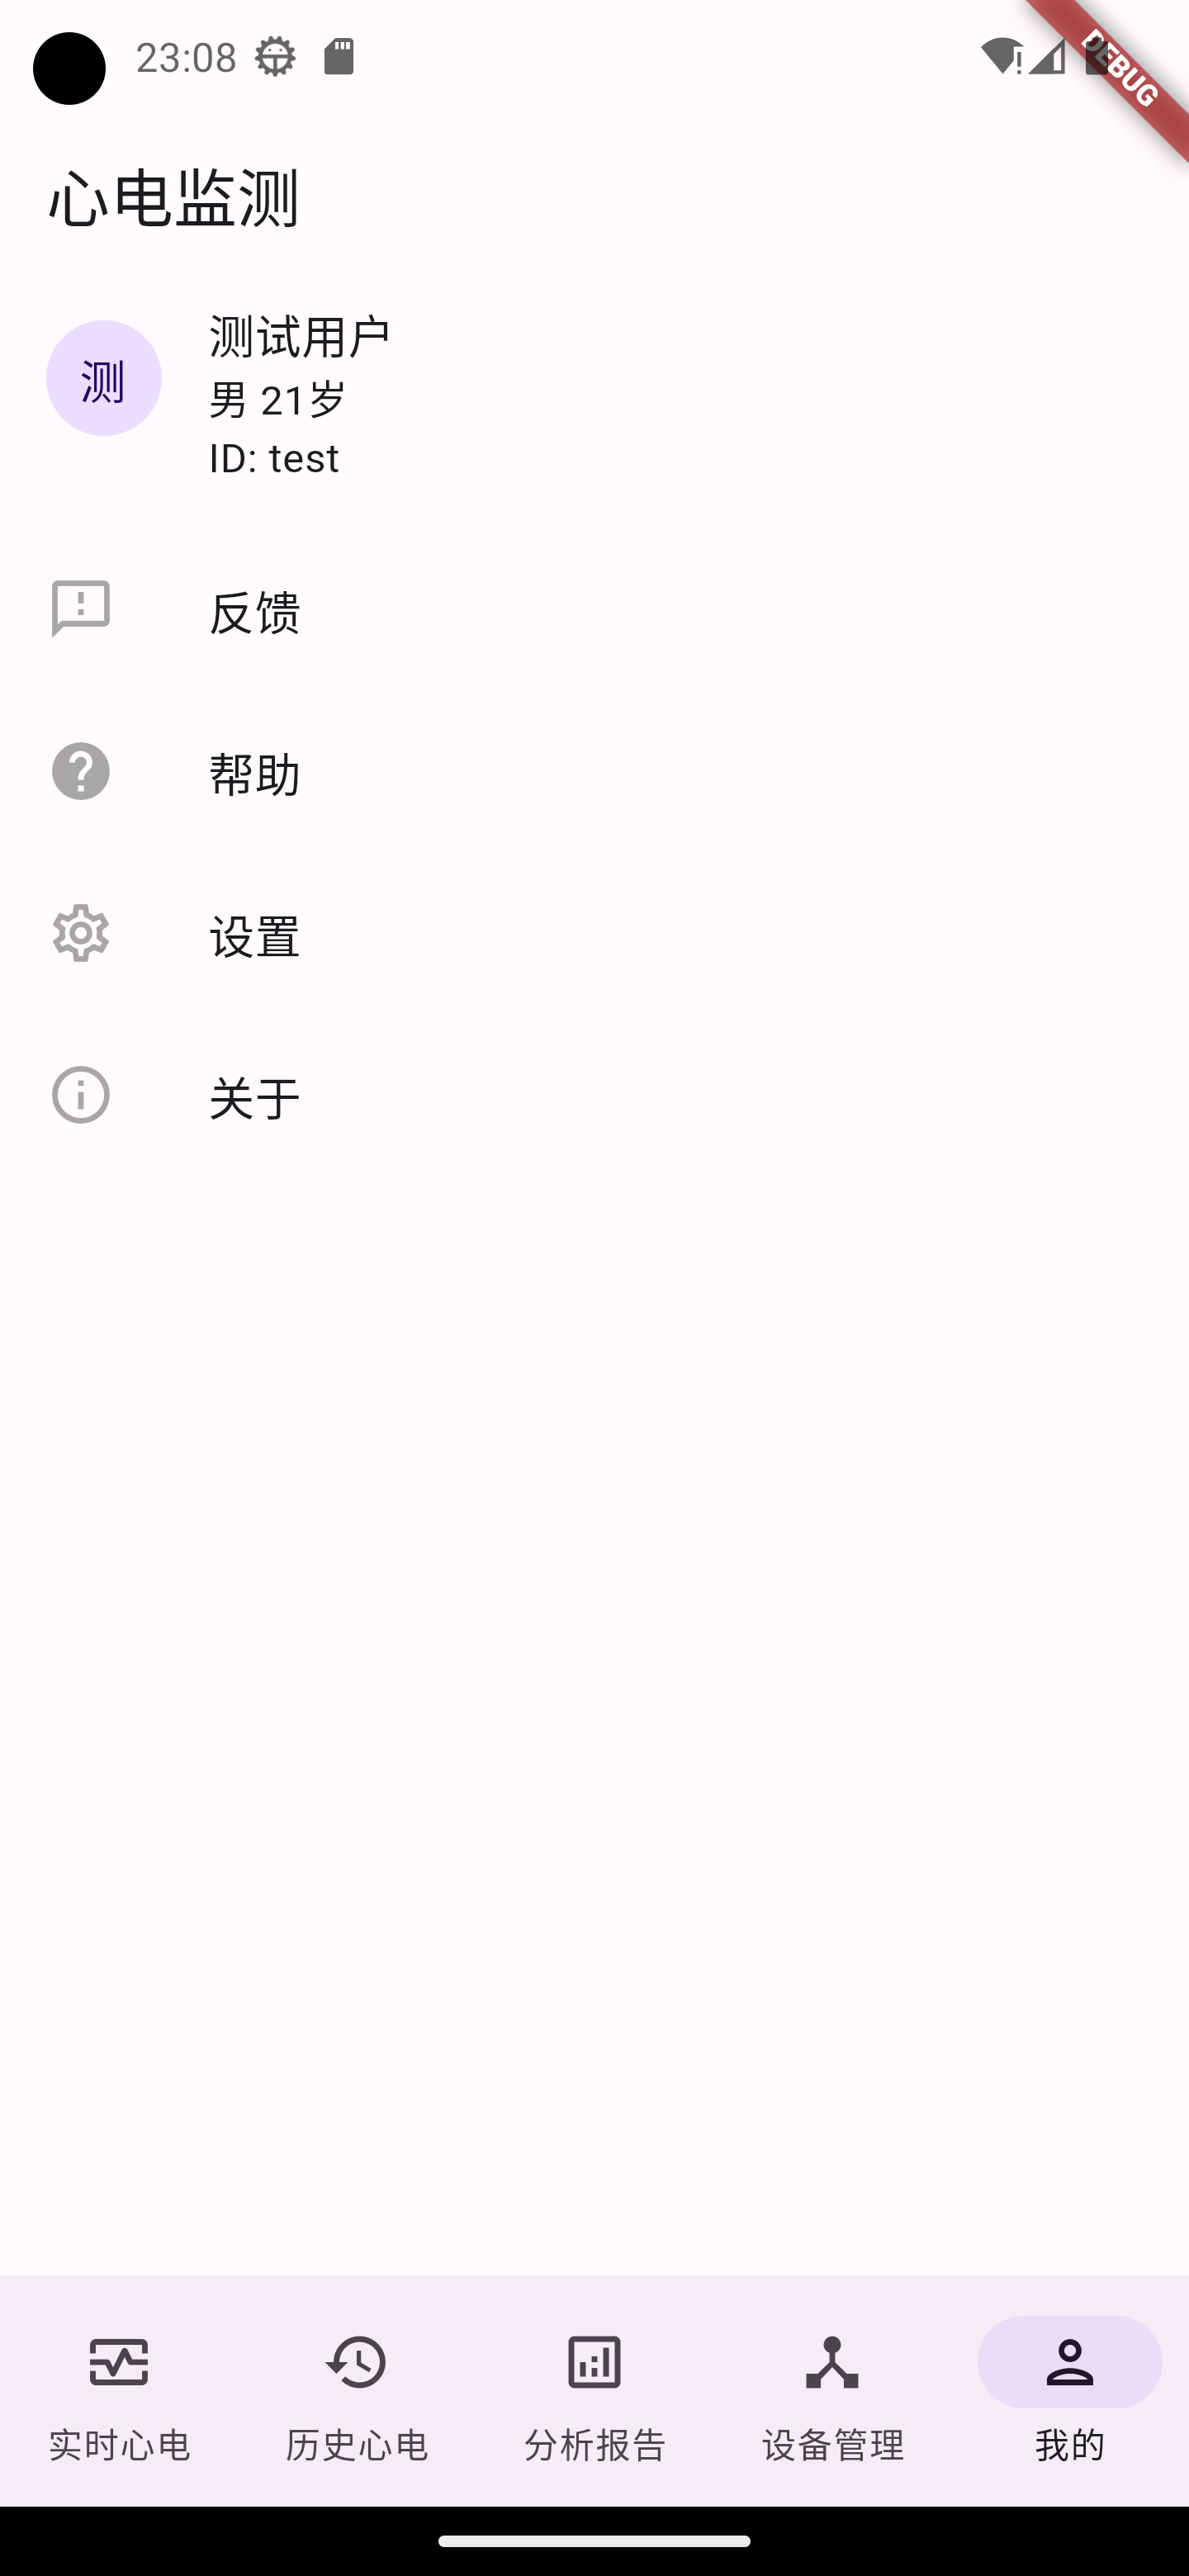
\includegraphics[width=.33\textwidth]{../assets/me}}
    \subcaptionbox{设置}{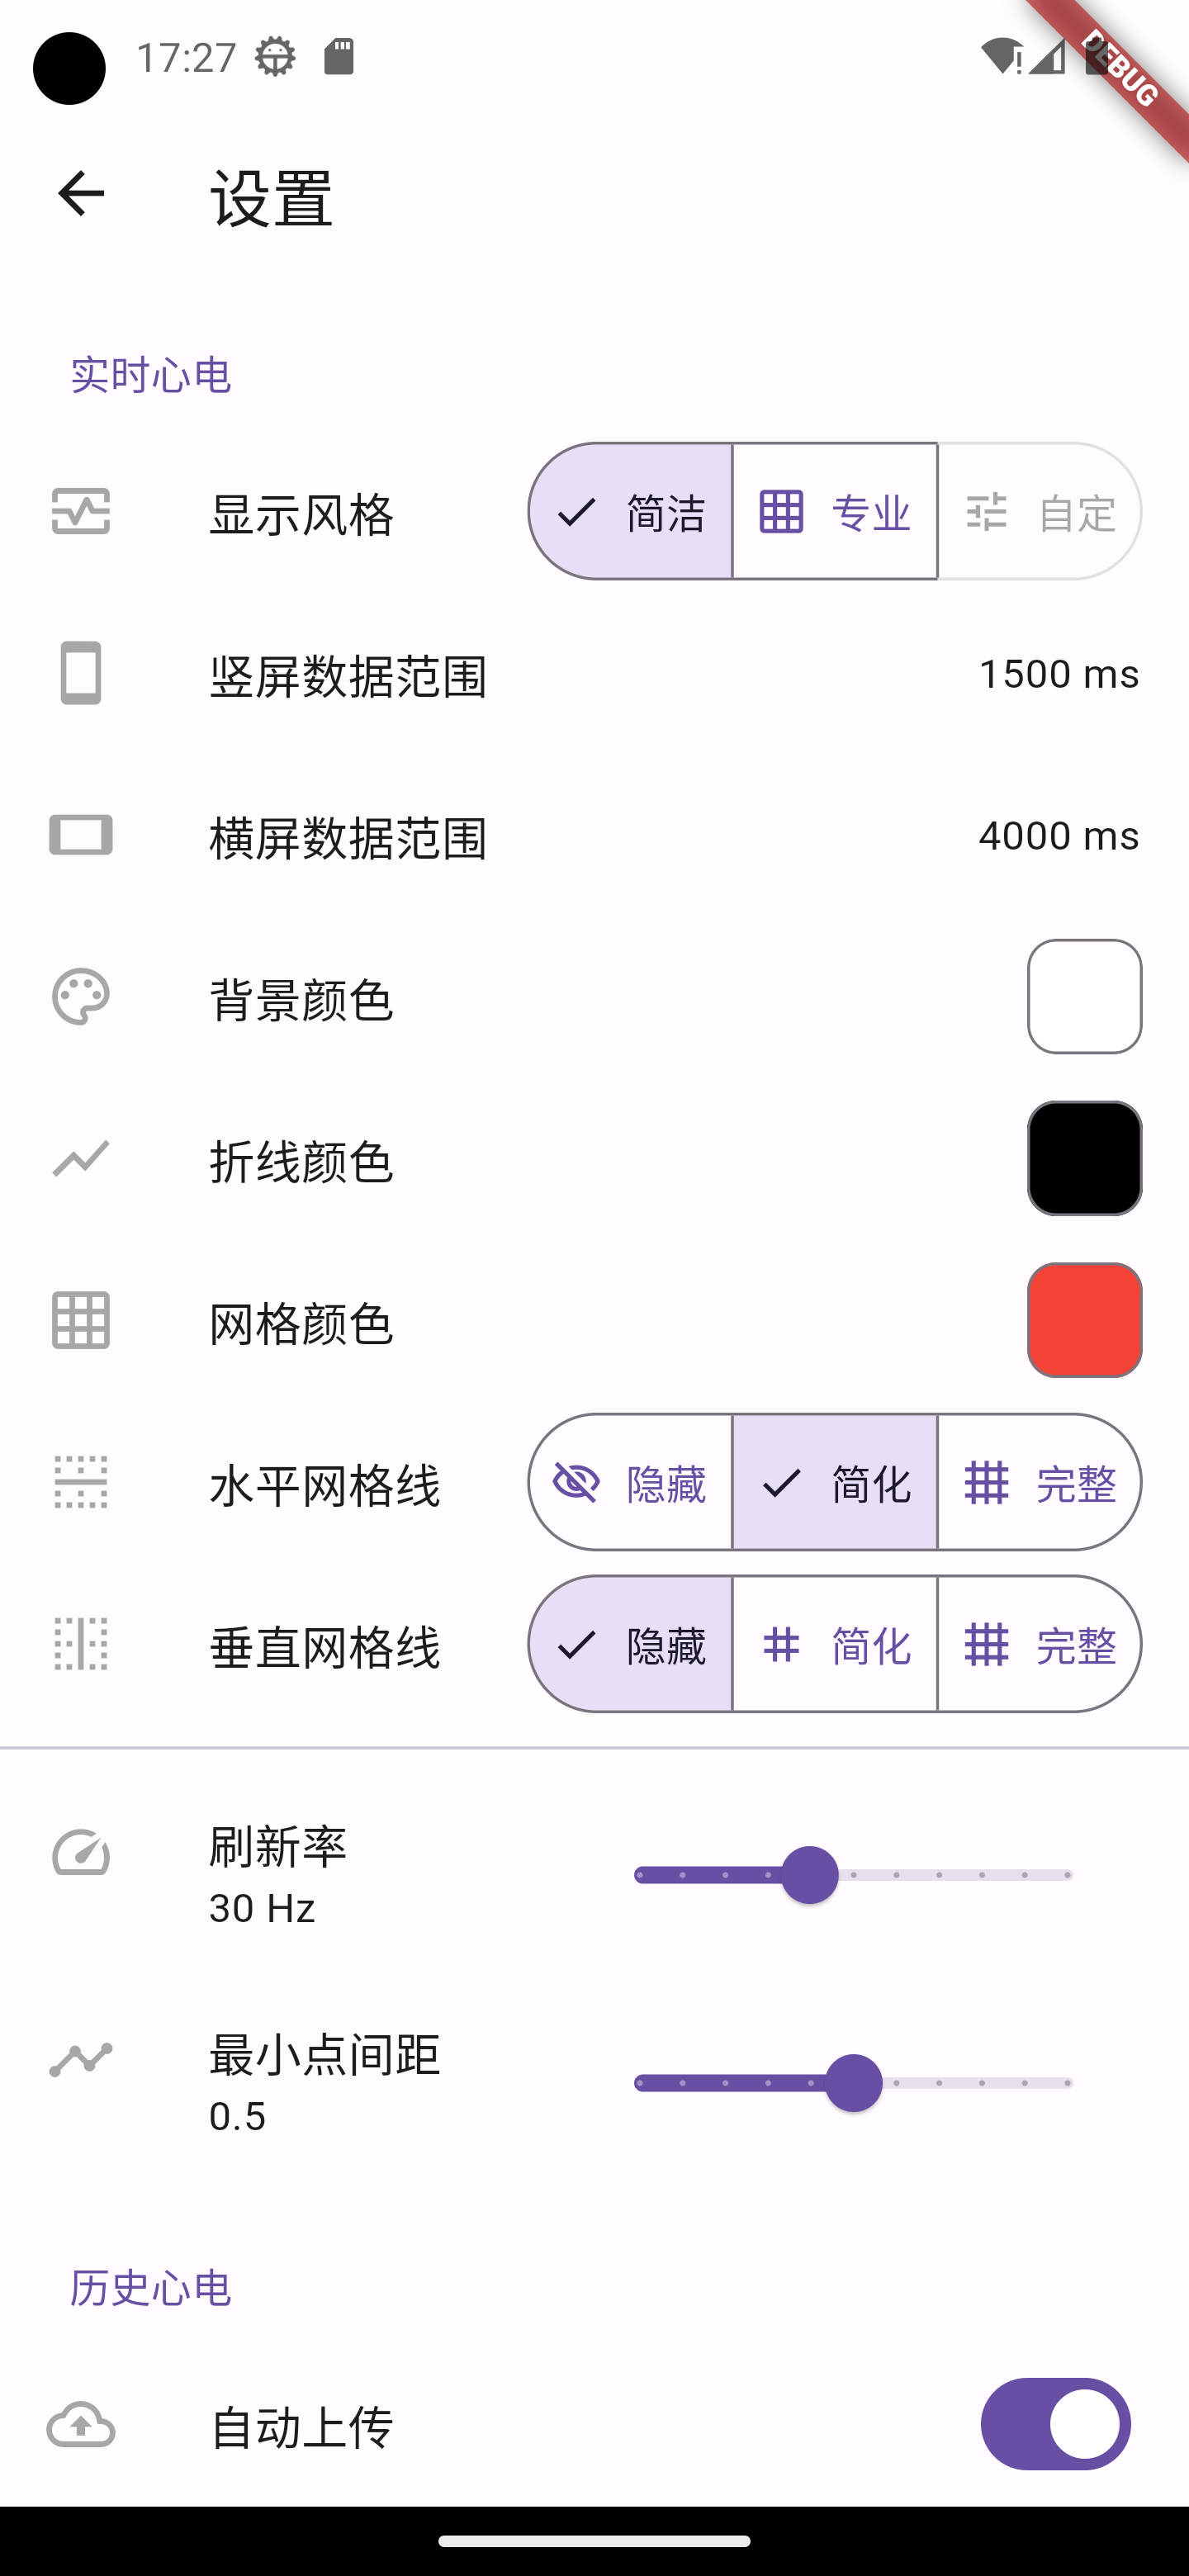
\includegraphics[width=.33\textwidth]{../assets/settings}}
    \subcaptionbox{许可}{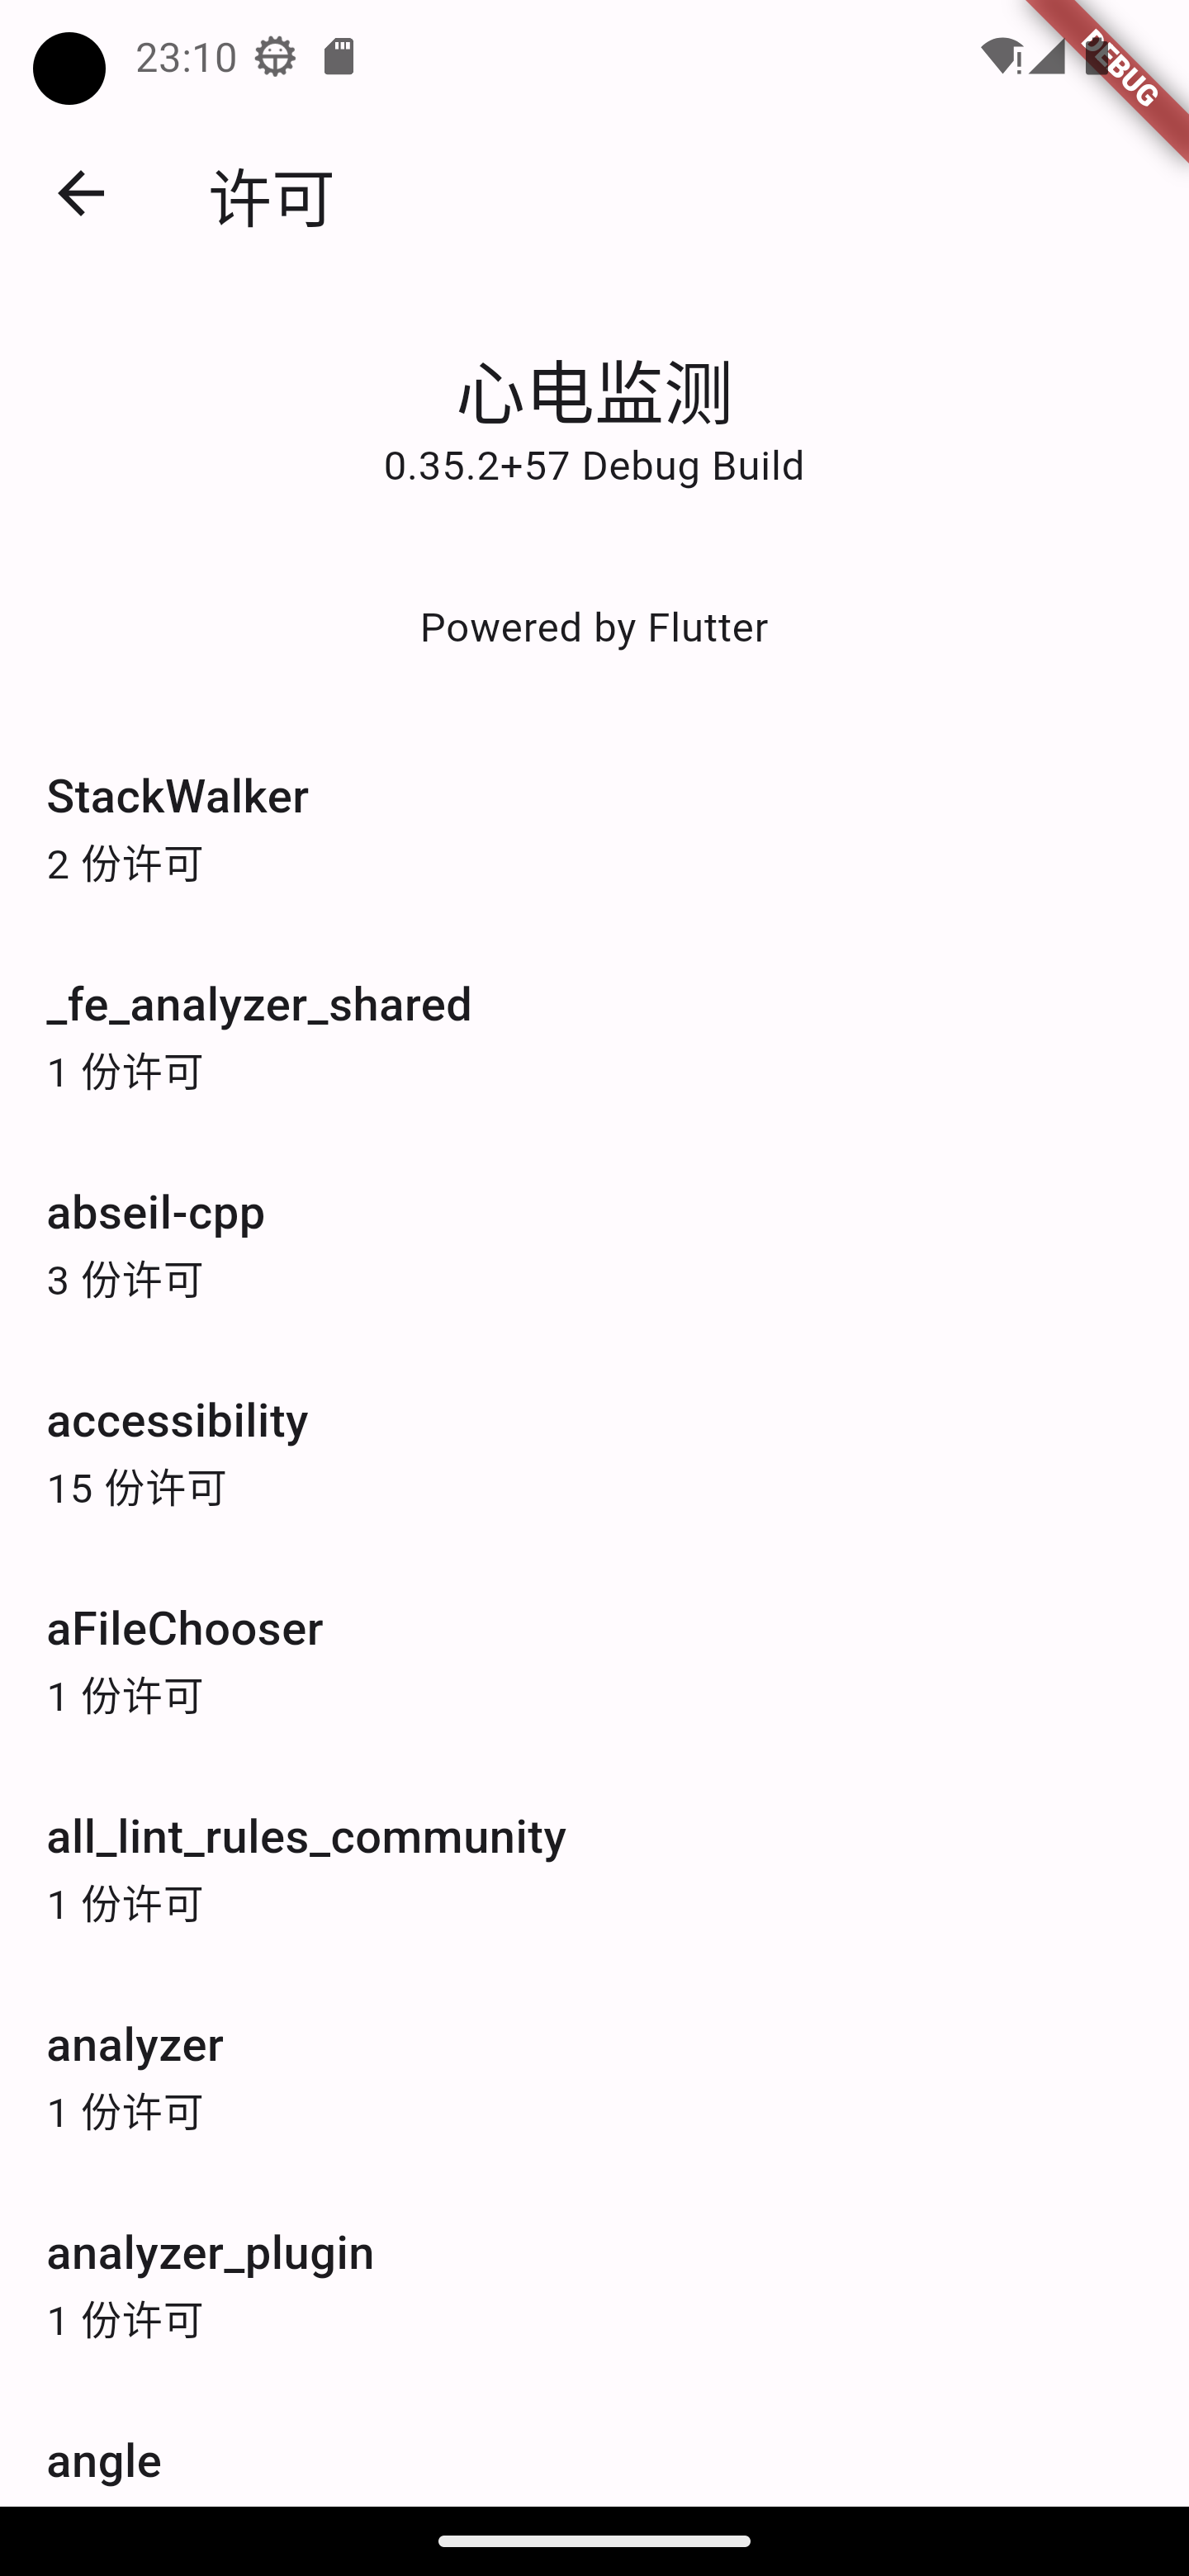
\includegraphics[width=.33\textwidth]{../assets/license}}
    \bicaption{部分其他界面的截图}{Screenshot of the some other pages}
    \label{fig:other}
\end{figure}

\subsection{我的界面的实现}\label{subsec:me-ui}

我的界面提供了其他所有界面的入口,在导航栏中的图标是用户头像的抽象表示。该界面以列表形式展示其内容。用户项目显示了当前用户的头像、姓名、性别、年龄、ID等信息,由于可以复用Web端(同课题下的另一个子项目)的用户管理相关的内容,所以并未对用户界面进行专门设计。反馈、帮助按钮会在点击后打开对应的网页。设置按钮会在点击后打开设置界面。关于按钮会在点击后显示包含应用自身的版本、构建模式等信息的对话框,并提供更新日志与许可信息的入口。

\subsection{应用设置模块的实现}\label{subsec:settings}

应用设置界面为常见的列表形式,划分为多个部分,每部分有一个小标题。设置项目均使用了图标、标题、输入组件的形式来展示,有部分如滑动条等的设置项目因不方便在输入组件直接展示当前状态而添加了副标题。而颜色选择器等所需面积较大的输入组件则有缩小形式与完整形式,缩小形式仅指示当前状态,点击后会在弹出的对话框中显示完整形式。

\todo{应用设置模块的更多实现细节}

\subsection{许可界面的实现}\label{subsec:license-ui}

通常而言,用户并不会有查看应用程序所使用的各个开源包的许可协议的需求。但是,由于多数许可协议要求在应用程序中提供许可协议的副本,因此应用程序中必须提供该界面的入口。该界面以列表形式展示其内容。许可界面的每一项都是一个开源包,点击后会在弹出的界面中显示该开源包的名称、作者、许可协议等信息。此外,该界面的上方也显示了本应用的名称、版本和构建模式的信息,并显示了“Powered by Flutter”的标识。

\subsubsection{应用自身信息的获取}\label{subsubsec:app-info}

\todo{应用自身信息的获取}

\subsection{界面过渡动画的实现}\label{subsec:transition-ui}

界面过渡动画是连接单个元素或应用程序全屏视图的短动画,是出色的用户体验的基础,可以帮助用户感知到应用程序的界面设计逻辑。由于在无法插入动态图片或视频的情况下较难充分展示界面过渡动画的实际效果,因此本文只作简短说明。

应用在心律类型详情界面的开启与关闭过程中使用了容器转换。当用户点击心律类型区域后,该区域会逐渐扩展至全屏,并将内容渐变为心律类型详情内容,关闭时则反之。这使得各个界面之间的关系清晰明确,加强了分析报告界面与心律类型详情界面的关联感。

在历史心电的所选时间改变后,使用了水平滑动效果,以提醒用户心电图是发生了水平移动。由于各个心拍之间的图像可能较为相似,如果没有该动画,用户可能会产生心电图发生了微小变形而非水平移动了一个心拍的错觉。

点击导航栏跳转至对应界面时使用了顶级(Top level)转换效果。该效果专门用于在应用程序的顶级目的地之间导航时,比如点击导航栏中的按钮时。该效果会将旧屏幕快速淡出,然后新屏幕快速淡入。由于顶级目的地的内容不一定相关,因此该动画效果有意不使用分组或持久元素来在屏幕之间创建牢固的关系。

\todo{界面过渡动画的更多实现细节}

\subsection{数据自动上传与自动删除的实现}\label{subsec:data-auto-ui}

应用每天会自动上传历史心电数据与分析报告结果至服务器(服务器端属于同课题的另一个子项目)。由于历史心电数据量较大而分析报告数据量较小,应用在设置中为两者的上传提供了分别的开关,以便流量有限的用户可以选择仅上传分析报告。

因为移动设备存储空间较为有限,所以应用会自动删除较旧的数据。应用删除数据的范围是距离当前时间超过两天的数据,而非一天,这是出于两点考虑:其一是因为应用内各界面最远提供了一天前的数据查询功能,如果在查询过程中进行删除,需要进行额外的加锁等考虑,而且可能会导致查询结果不准确;其二是因为应用在自动上传数据时可能会因为网络等原因失败,将数据额外保留一天可以提供一些重试的机会。

\todo{数据自动上传与自动删除的更多实现细节}

\subsection{应用的无障碍功能实现}\label{subsec:accessibility-ui}

图~\ref{fig:accessibility} 展示了应用的一些无障碍功能。

\begin{figure}[ht]
    \subcaptionbox{界面放大}{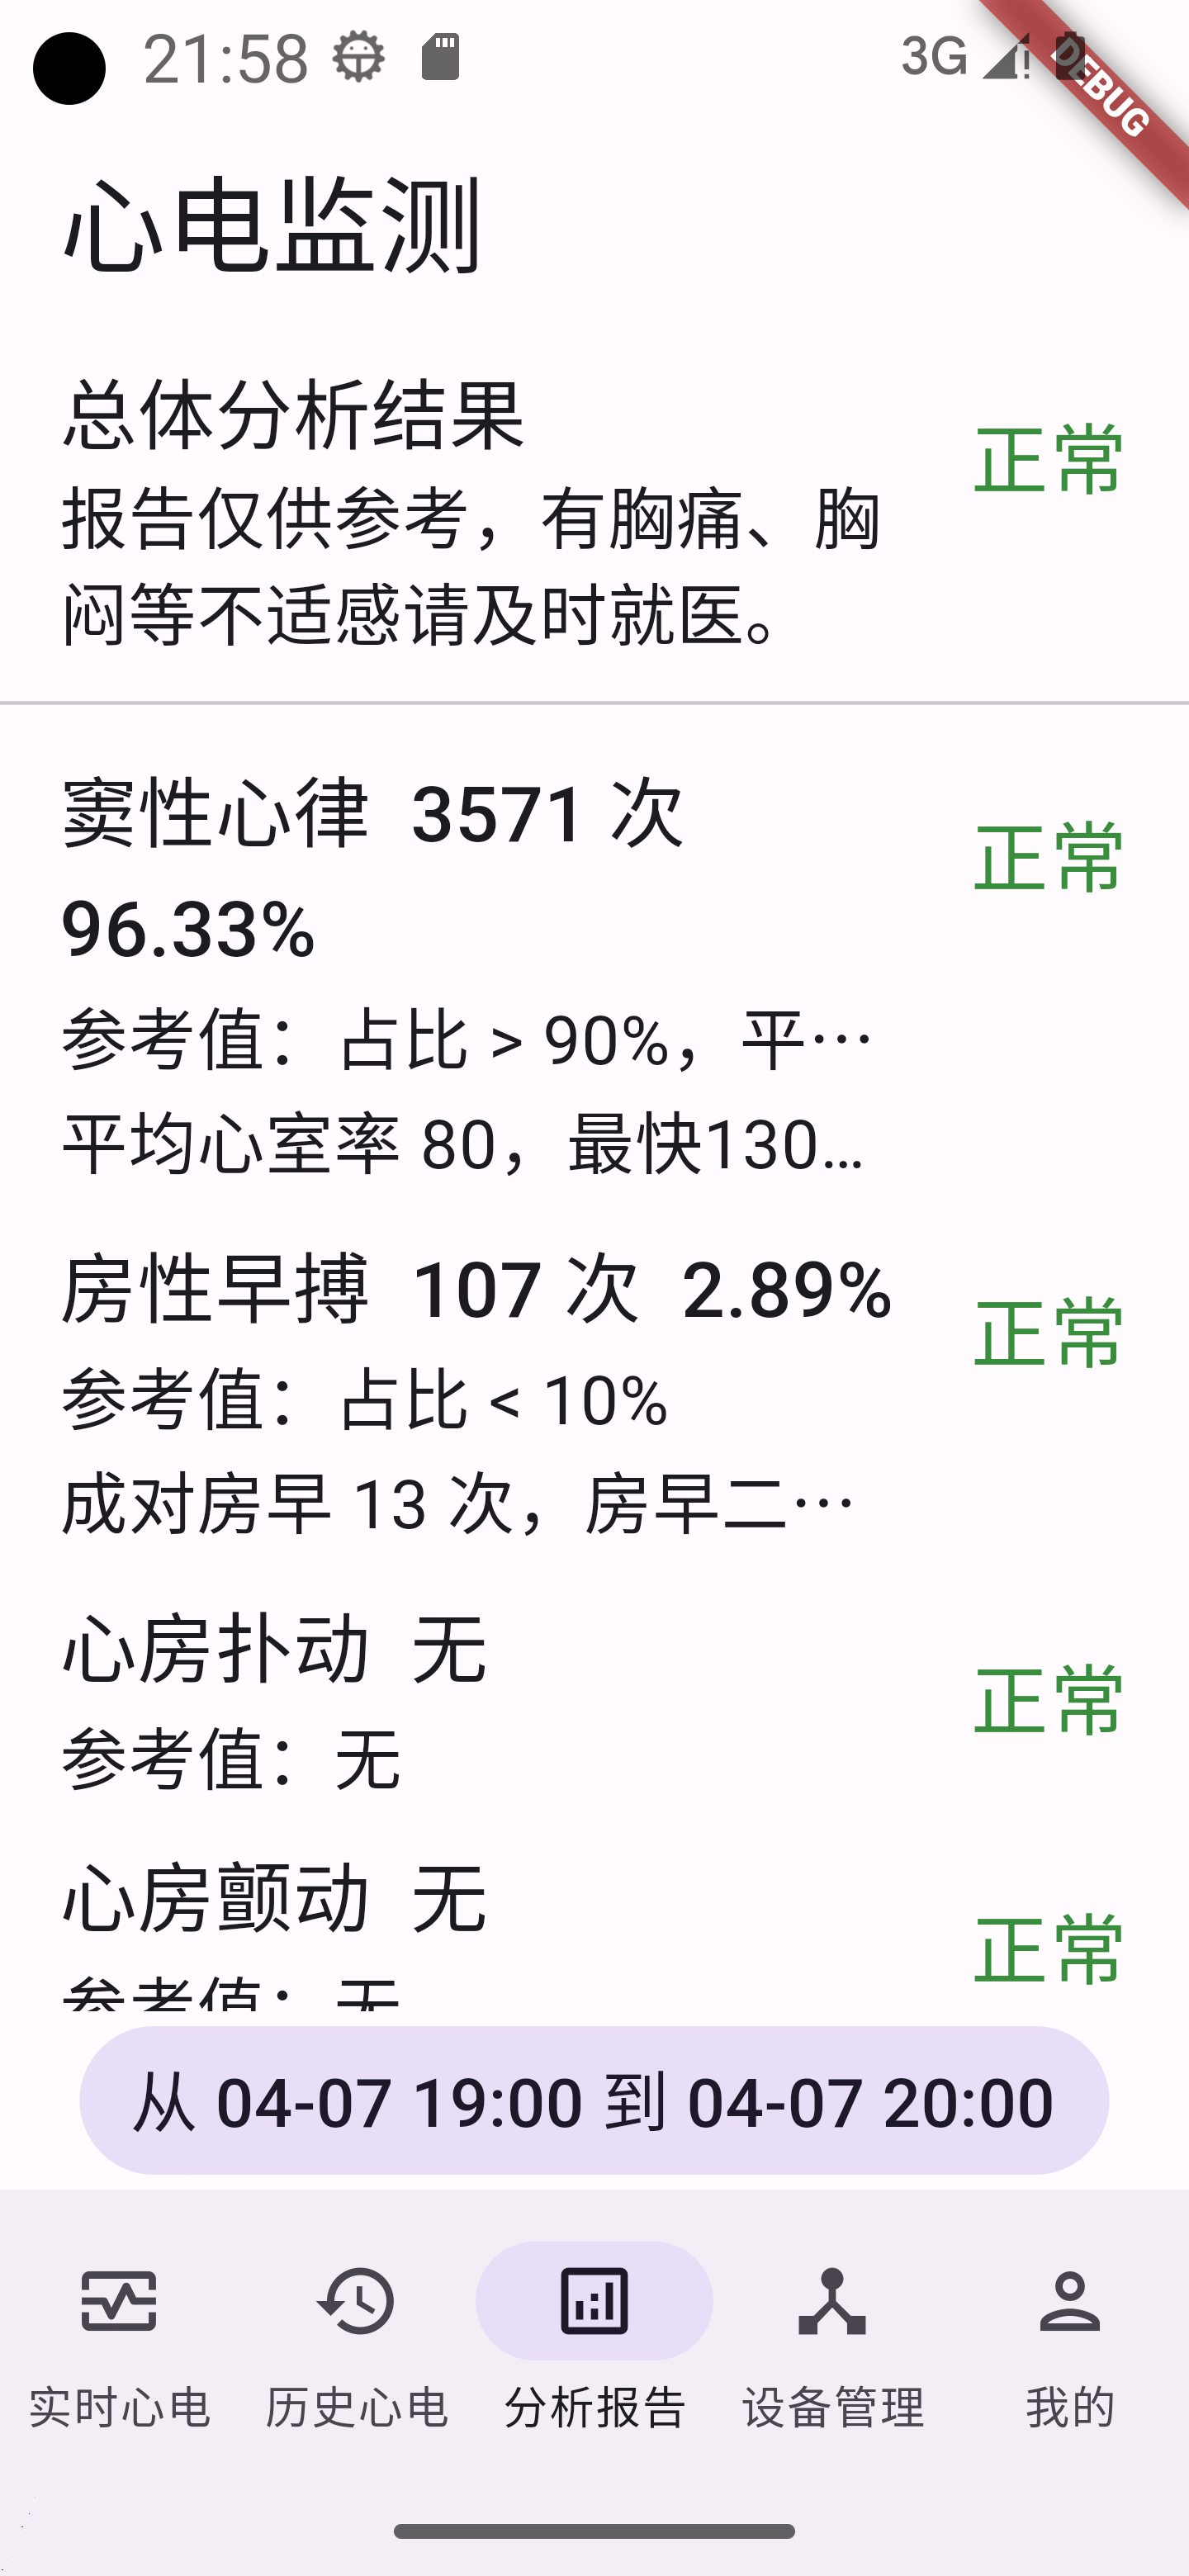
\includegraphics[width=.33\textwidth]{../assets/big}}
    \subcaptionbox{粗体高对比度}{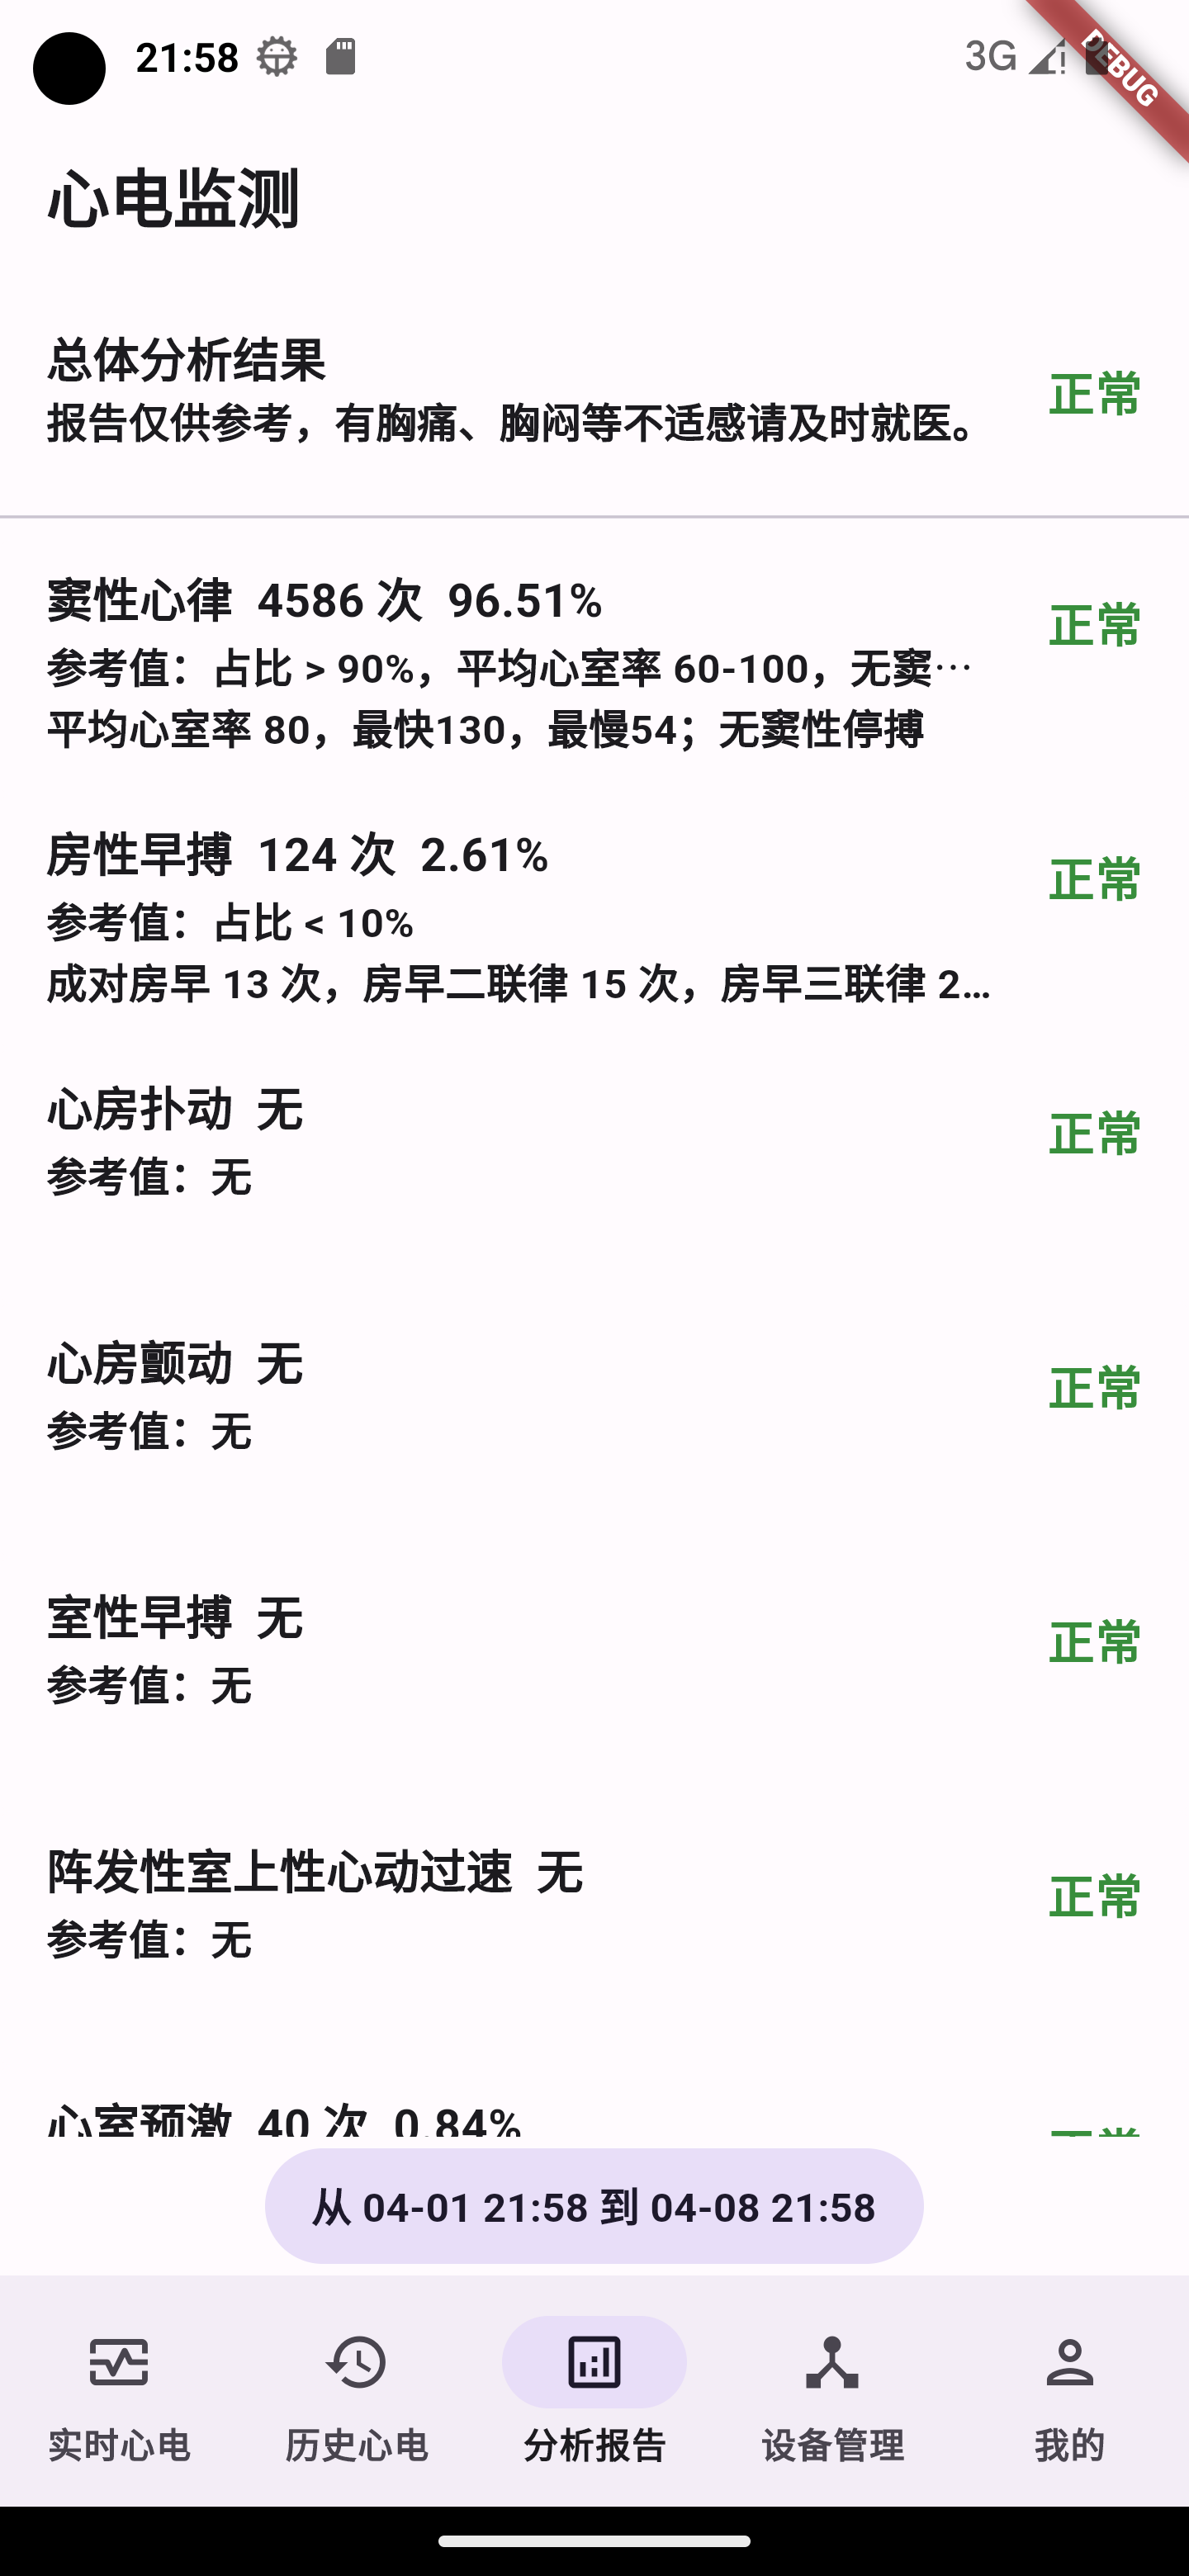
\includegraphics[width=.33\textwidth]{../assets/bold}}
    \subcaptionbox{深色模式}{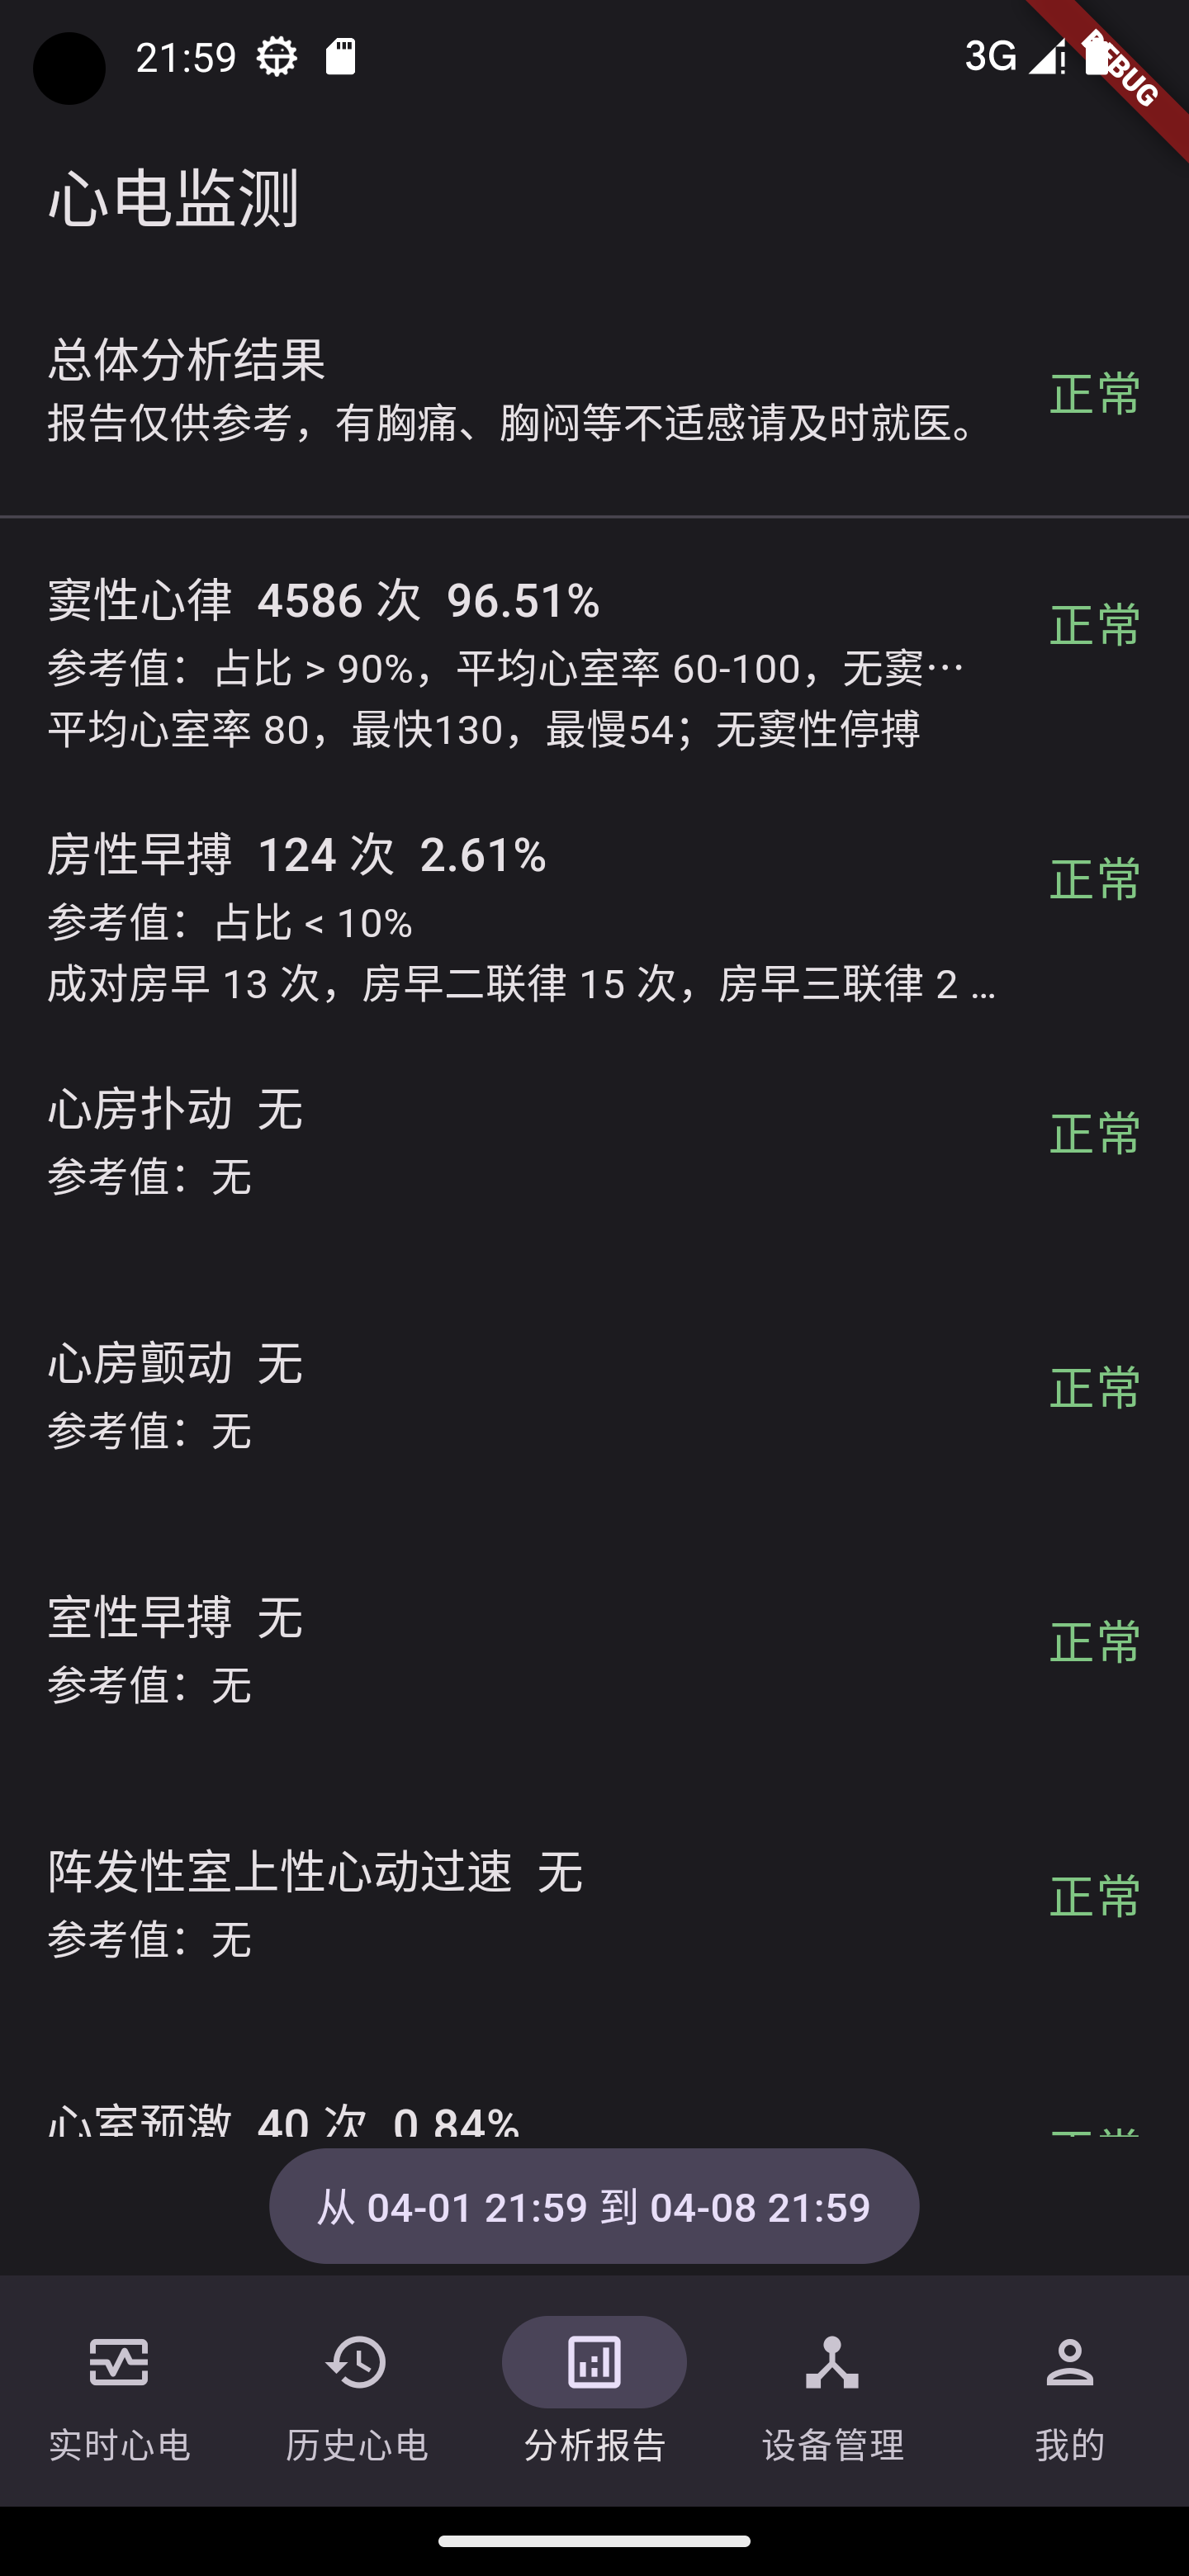
\includegraphics[width=.33\textwidth]{../assets/dark}}
    \bicaption{应用的无障碍功能}{Accessibility of the app}
    \label{fig:accessibility}
\end{figure}

当用户开启了界面放大后,应用内一些原本在一行之内显示的文本会无法在一行内完整显示。对于有必要完全显示出来的内容,应用会将其进行换行,在多行之中显示。对于没有必要完全显示的内容,应用会将其折叠,以省略号指示内容未显示完全。通过这些处理,应用在界面放大的状态下虽然美观程度略有下降,但功能都可以保证正常使用。界面放大的一个常用替代方式是将文本加粗加黑,应用在这种情况下也可以正常提供功能。

为了支持深色模式与浅色模式的切换,应用在设计中尽量避免了使用固定的颜色,而是使用系统上下文提供的颜色。这样,应用在不同的主题下自然都可以随之自动切换颜色,从而正常显示内容。

\subsection{平台自适应UI的实现}\label{subsec:adaptive-ui}

\subsubsection{应用UI遵循的规范}

本应用在UI方面与其他同类应用的一大差别在于其遵循专业的规范对UI元素的使用进行了精细的考虑。

应用整体上遵循Material 3规范\cite{MaterialDesign}。Material 3(也称为Material You)是Google在2021年5月的Google I/O大会上宣布的新一代Material规范,和前代规范相比具有从用户的壁纸自动生成动态主题颜色、按钮更大、界面动画更多等新特性,并在其他一些细节上有所优化。目前Material 3规范已被广泛应用于Google的各种应用程序,并成为Android应用的推荐UI规范。

尽管Material 3按照Google的设计是可以在任何平台(包括iOS)上使用的,但从事实上来说,iOS应用确实较少使用Material风格的UI,而较多按照苹果的推荐遵循Cupertino\footnote{苹果官方并未给自己的UI规范进行像Material这样的明确命名,Cupertino这个名字是Flutter在其文档中使用的,可能是基于苹果总部位于美国加利福尼亚州丘珀蒂诺(Cupertino)市的事实。}规范。

\subsubsection{应用在不同平台的UI对比}

为了符合iOS平台的用户习惯,本应用基于Flutter Platform Widgets包在iOS平台上将部分UI组件替换为了iOS应用常用的Cupertino风格的组件。由于Cupertino并未像Material一样设计为全平台可用,所以应用的UI风格仍然以Material为主,在Android平台上完全使用Material 3风格的UI,而在iOS平台上则使用Material 3风格与Cupertino风格的混合,如图~\ref{fig:android-ios} 所示。

\begin{figure}[ht]
    \centering
    \subcaptionbox{Android}{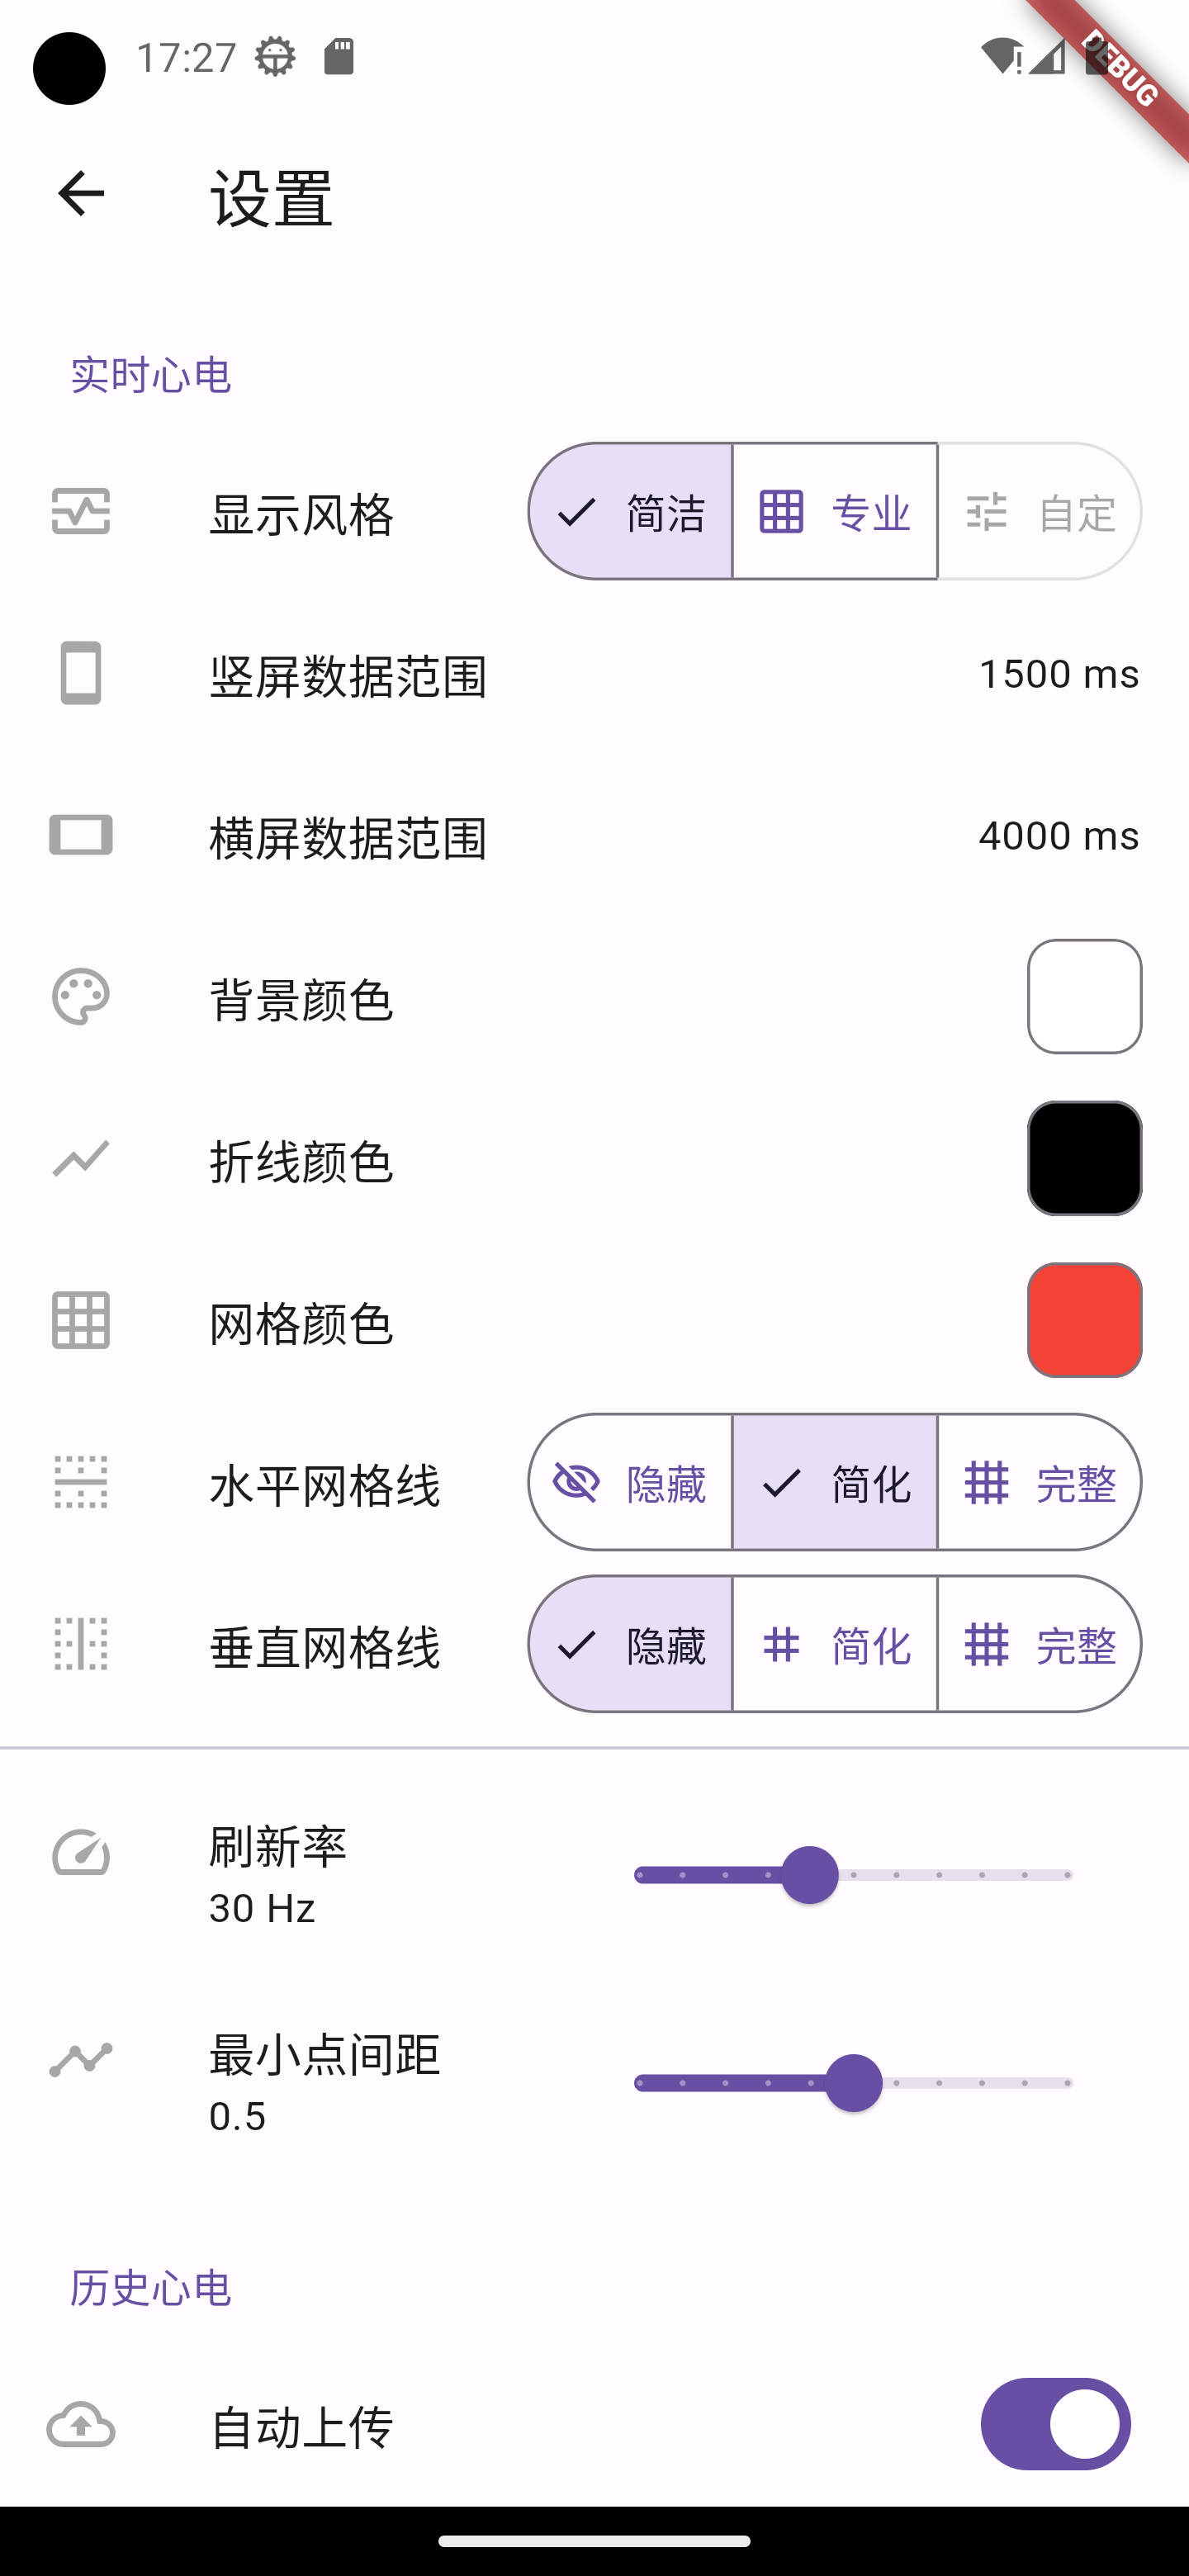
\includegraphics[height=13cm]{../assets/settings}}
    \subcaptionbox{iOS}{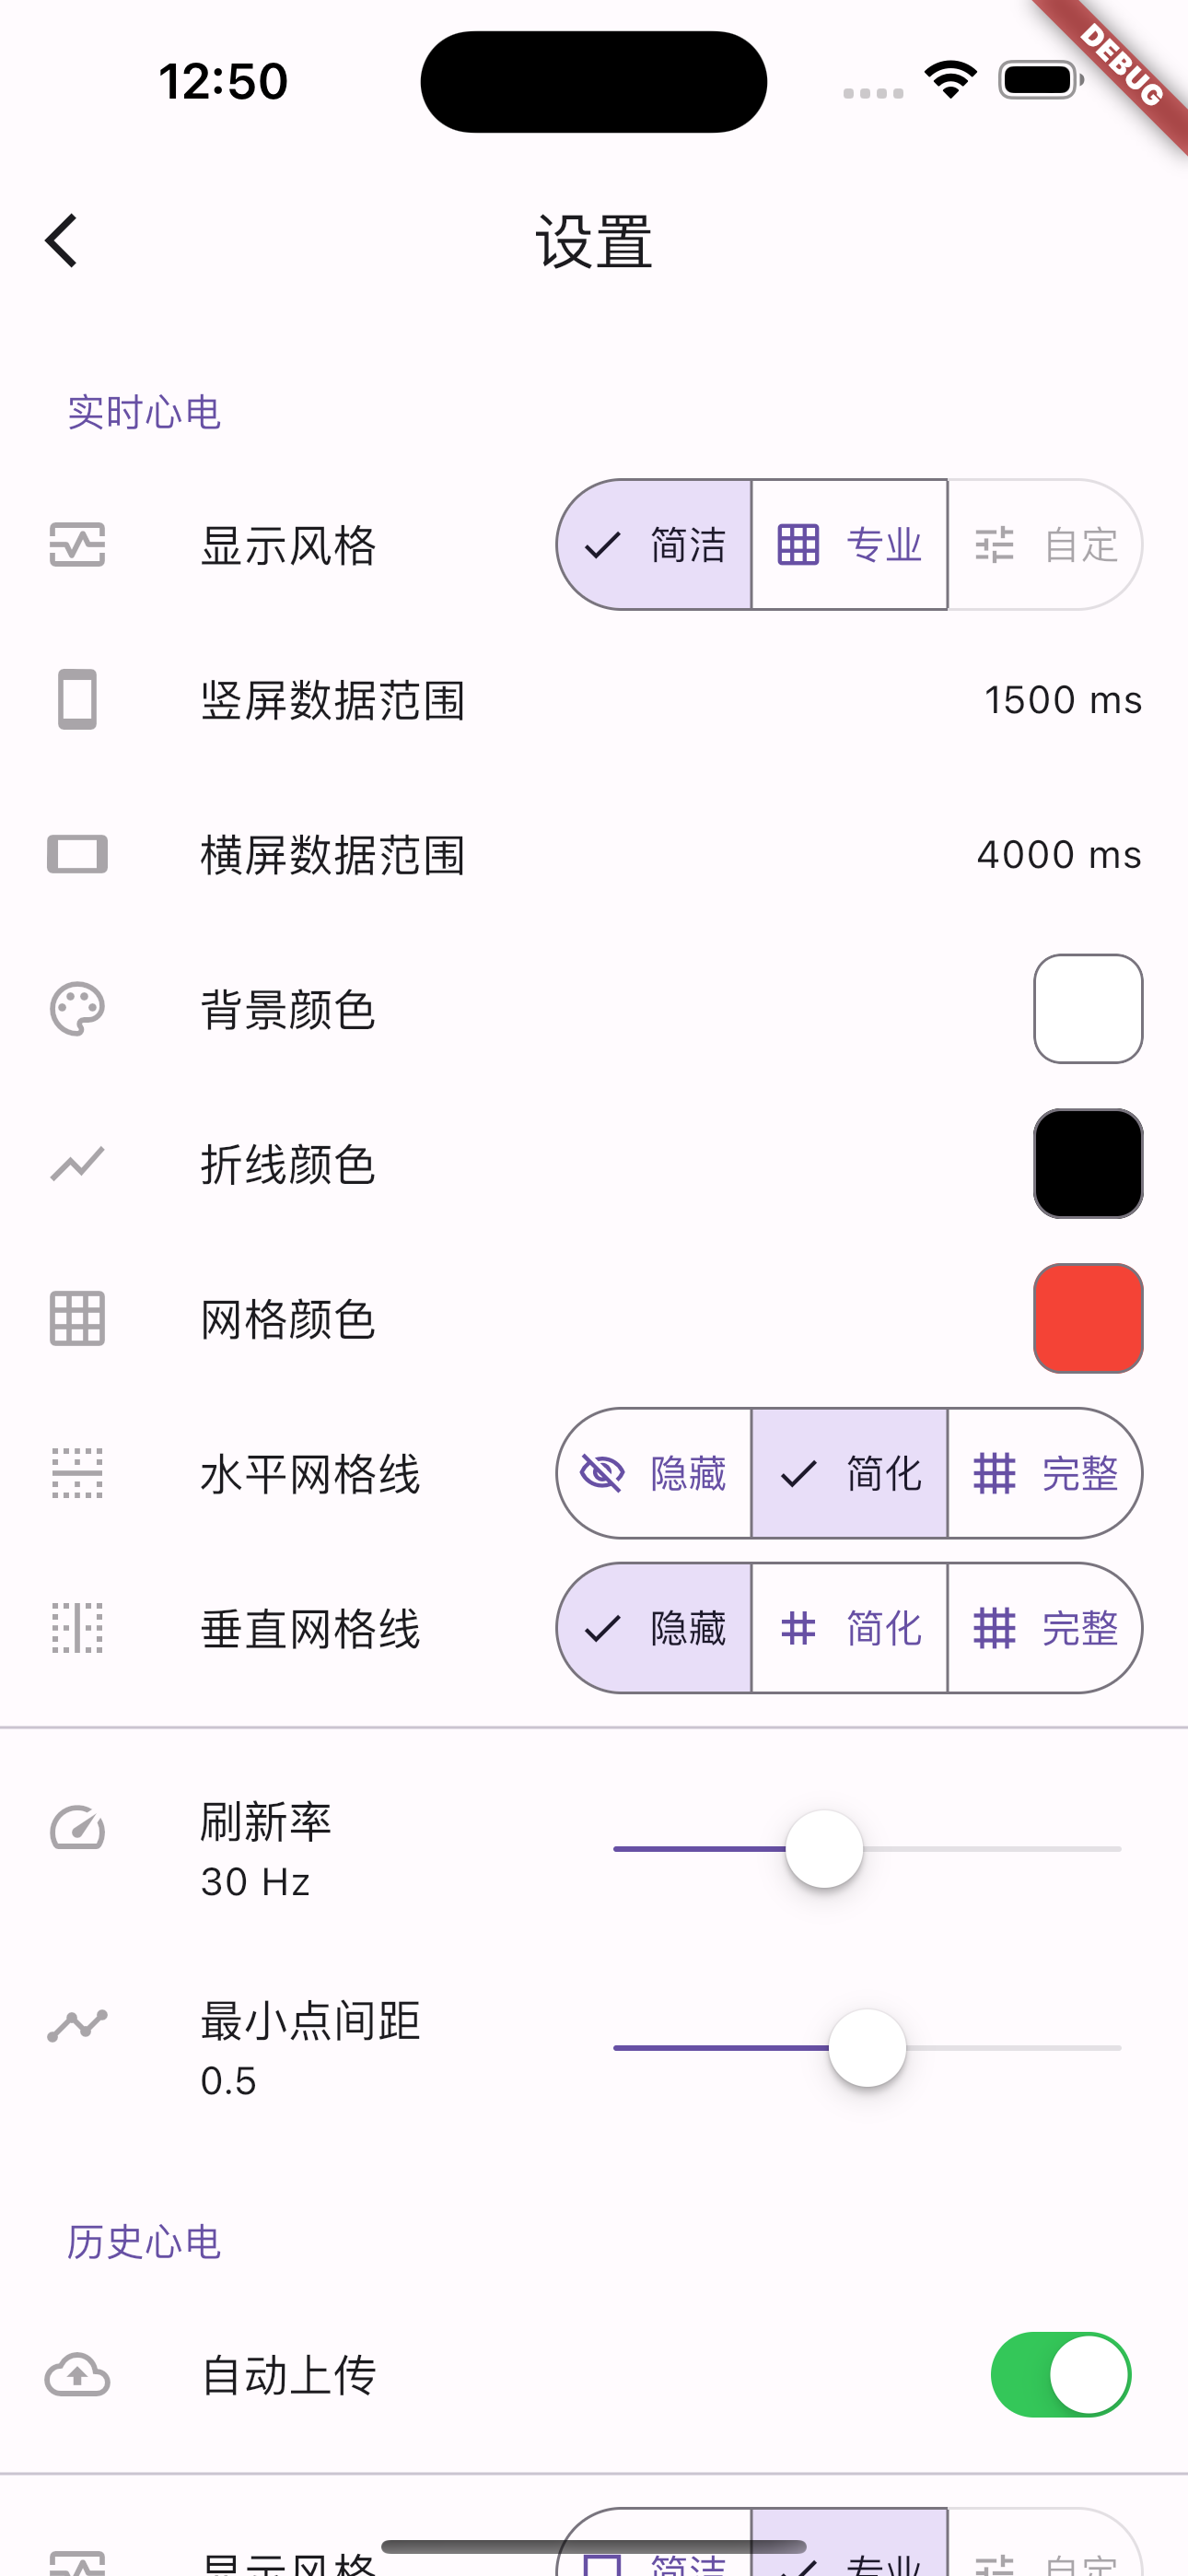
\includegraphics[height=13cm]{../assets/ios-settings}}
    \bicaption{应用在Android和iOS平台上的UI对比}{Comparison of the app's UI on Android and iOS}
    \label{fig:android-ios}
\end{figure}

从图中可以看出应用在Android平台与iOS平台上的UI实现上的一些差异,包括标题的对齐方式(Android居左,iOS居中)、左上角返回按钮的图标(Android使用完整箭头,iOS使用仅有头部的简化箭头)、滑动条与切换按钮的外观(按照各自规范中的相关要求)、文本的字体(iOS的字体更细)等。

\subsubsection{Flutter Platform Widgets包在实现中的作用}

Flutter Platform Widgets包在平台自适应UI的实现中起到的作用主要在于基于共识消除了不必要的样板代码。比如为了在Android平台和iOS平台使用不同的滑动条外观,原本需要在 |if| 条件中通过判断 |Platform.isAndroid| 或 |Platform.isIOS| 来决定使用 |Slider| 还是 |CupertinoSlider|。由于 |Slider| 和 |CupertinoSlider| 是公认的不同风格设计对同一种UI的实现,相关的代码并没有提供任何额外的信息量,只是无意义的冗余。使用Flutter Platform Widgets包后,只需要使用 |PlatformSlider| 即可,其内部会根据平台自动选择使用 |Slider| 还是 |CupertinoSlider|。这不仅避免了大量关于平台判断的 |if| 语句,也避免了将相同的参数分别传递至两个平台对应的类的构造函数之中,有助于使代码更加简洁。

\subsection{路由功能的实现}\label{subsec:router}

\todo{路由功能的实现}

\subsection{本地化功能的实现}\label{subsec:l10n}

\todo{本地化功能的实现}

\subsection{开发者工具的实现}\label{subsec:dev-tools}

\todo{开发者工具的实现}

\subsubsection{日志功能的实现}\label{subsubsec:log}

\todo{日志功能的实现}
